%!TEX TS-program = pdflatex
\documentclass[iop]{emulateapj}

\usepackage{amssymb,graphics} % for resolution symbol and \blacktriangledown
\usepackage{longtable,booktabs,multirow}
\usepackage{wasysym} % for \astrosun

\maxdeadcycles=1000
\setcounter{secnumdepth}{5}

\shorttitle{The Aquarius Co-Moving Group is Not a Disrupted Classical Globular Cluster}
\shortauthors{Casey et al}

\begin{document}

\title{The Aquarius Co-Moving Group is Not a Disrupted Classical Globular Cluster\altaffilmark{1}}

% TODO:
% - Uncertainty analysis for a standard star
% - Uncertainty analysis for a prgram star

\author{Andrew R. Casey\altaffilmark{2,3}, Stefan Keller\altaffilmark{2}, Alan Alves-Brito\altaffilmark{2,4}, Anna Frebel\altaffilmark{3}, Gary Da Costa\altaffilmark{2}, Amanda Karakas\altaffilmark{2}, David Yong\altaffilmark{2}, Kevin Schlaufman\altaffilmark{3}, Heather R. Jacobson\altaffilmark{3}, Qinsi Yu\altaffilmark{3}, Cherie Fishlock\altaffilmark{2}}
\altaffiltext{1}{This paper includes data gathered with the 6.5 meter Magellan Telescopes located at Las Campanas Observatory, Chile.}
\altaffiltext{2}{Research School of Astronomy and Astrophysics, Australian National University, Canberra, ACT 2611, Australia; acasey@mso.anu.edu.au}
\altaffiltext{3}{Massachusetts Institute of Technology, Kavli Institute for Astrophysics and Space Research,
77 Massachusetts Avenue, Cambridge, MA 02139, USA}
\altaffiltext{4}{Departamento de Astronom\'ia y Astrof\'isica, Ponticia Universidad Cat\'olica de Chile, Av. Vicu\~na Mackenna 4860, Macul, 782-0436 Santiago, Chile}


\begin{abstract}
\noindent{}We present a detailed analysis of high $S/N$, high-resolution spectra for 5 Aquarius stream stars observed with the MIKE spectrograph on the Magellan Clay telescope. Our sample represents one third of the 15 members in the stream. We find the stream is not mono-metallic; the metallicity ranges from [Fe/H] = $-$0.63 to $-$1.58 dex. No anti-correlation in Na-O abundances is present, and we find a strong positive Mg-Al relationship, similar to that observed in the thick disc. We find no evidence that the stream is a result of a disrupted classical globular cluster, contrary to a previously published claim. High [(Na, Ni, $\alpha$)/Fe] and low [Ba/Y] abundance ratios in the stream suggests it is not a tidal tail from a disrupted dwarf galaxy, either. The stream is chemically indistinguishable from Milky Way field stars with the exception of one candidate, C222531-145437. From its position, velocity, and detailed chemical abundances, C222531-145437 is likely a star that was tidally disrupted from $\omega$-Centauri. We propose the Aquarius stream is galactic in origin, and could be the result from a disc-satellite perturbation in the Milky Way thick disc on the order of a few gigayear ago. Derived orbits, $UVW$ velocities, and angular momenta of the Aquarius members offer qualitative support for our hypothesis. Assuming C222531-145437 is a tidally disrupted member of $\omega$-Centauri, this system is the most likely disc perturber. In the absence of compelling chemical and/or dynamical evidence that the Aquarius stream is the tidal tail of a disrupted satellite, we advocate the ``Aquarius group'' as a more appropriate description. Like the Canis Major over-density, as well as the Hercules and Monoceros groups, the Aquarius group adds to the list of kinematically-identified substructures that are not actually accreted material; they are simply part of the rich complexity of the Milky Way structure.
\end{abstract}

\keywords{Galaxy: halo, structure}

\section{Introduction}
Galaxies are formed hierarchically through chaotic mergers of smaller systems, and the Milky Way is no exception \citep{bullock;johnston_2005,helmi_2008}. The accumulating stellar debris in our own Galactic halo provides ongoing evidence for such merging events \citep[e.g.][]{bell;et-al_2008}. As satellites fall towards the Galaxy, tidal forces disrupt the system, hurtling stars in leading and trailing directions. The position and velocities of stars within these ``stellar streams'' are sensitive to the Galactic potential. As such, their phase-space information can collectively constrain the fraction and distribution of accreted matter in the galaxy, the sub-halo mass function, as well as the shape and extent of the Milky Way's dark matter halo. Additionally, individual chemical abundances can trace the chemical evolution of the Galaxy and its satellite systems.

Wide-field deep imaging surveys have proved excellent sources for finding stellar streams \citep[e.g.][]{belokurov;et-al_2007}. Dozens of streams have been identified through careful photometric selections and matched-filtering techniques, with some to a galactocentric distance of 100\,kpc \citep[e.g., see][]{drake;et-al_2013}. Indeed, it is clear that a large fraction of the stellar halo has been built up by accretion. However, as \citet{helmi;white_1999} point out, these detection strategies are most successful for identifying streams that are sufficiently distant from the solar neighbourhood. A nearby stream, within $\sim$10\,kpc, will not appear as a photometric over-density because the stars would be sparsely positioned across the sky. Such substructures would only be detectable by their kinematics, or perhaps with precise elemental abundances through a ``chemical tagging'' approach (e.g. see \citealt[][]{freeman;bland-hawthorn_2002}). The confirmation of such substructures would serve to substantially increase the fraction of the known accreted material in the Galaxy.

It is therefore necessary to spectroscopically survey stars in the solar neighbourhood to reveal any nearby substructures. The Radial Velocity Experiment (RAVE) team began such a survey in 2003 and has taken spectra of over 500,000 stars across 17,000\,deg$^{2}$ \citep{steinmetz;et-al_2006}. The primary goal of RAVE is to obtain radial velocities for stars in the solar neighbourhood and beyond. In an attempt to remain kinematically unbiased, RAVE candidates were selected solely by their apparent magnitude ($9 < I < 13$).  Almost all of these candidates have published radial velocities \citep{steinmetz;et-al_2006}, and for a subset of stars with a sufficient signal-to-noise ($S/N$) ratio, stellar parameters have been derived by a $\chi^2$-minimisation technique \citep{zwitter;et-al_2008, siebert;et-al_2011}. 

Using these data, \citet{williams;et-al_2011} identified a co-moving group of nearby (${0.5\,\mbox{kpc} \lesssim D \lesssim 10\,\mbox{kpc}}$) stars near ${(l, b) = (60^\circ, -55^\circ)}$, in the vicinity of the Aquarius constellation. Thus, the co-moving group was named the Aquarius stream. The stream is most apparent when examining heliocentric velocities against galactic latitude for stars within $-70^\circ < b < -50^\circ$. \citet{williams;et-al_2011} employed a selection criteria of $-250\,\mbox{km s}^{-1} < V_{\rm hel} < -150\,\mbox{km s}^{-1}$, $30^\circ < l < 75^\circ$ and $J > 10.3$ to maximize the contrast between the stream and stellar background, identifying 15 stars in the process. The average heliocentric velocity of these members was found to be $V_{\rm hel} = -199\,\mbox{km s}^{-1}$, with a dispersion of 27\,km s$^{-1}$. The radial velocity uncertainties provided by the RAVE catalog are described to be $\sim$2\,km s$^{-1}$, so the stream's wide velocity distribution appears to be real.

Through a statistical comparison with predictions of stellar positions and kinematics from the Galaxia \citep{sharma;et-al_2011} and Besan\c{c}on \citep{robin;et-al_2003} models of the Milky Way, \citet{williams;et-al_2011} found the stream \ to be statistically significant ($>4\sigma$). The choice of model, cell dimension, or extinction rate made no real difference to the detection significance. The authors concluded the over-density was genuine, and inferred that the co-moving group is a stellar stream. Based on the phase space information available, \citet{williams;et-al_2011} concluded that the newly discovered stream could not be positively associated with the Sagittarius or Monoceros stream, the Hercules-Aquila cloud, or either the Canis Major or Virgo over-densities. 

RAVE data suggest the Aquarius stream has a metallicity of [Fe/H] $= -1.0 \pm 0.4$\,dex\footnote{\citet{williams;et-al_2011} formally quote [M/H], but for the sake of a consistent discussion we assume [M/H] $\equiv$ [Fe/H] throughout this study.}, slightly more metal-rich than halo stars at the same distance (${\mbox{[Fe/H]} = -1.1 \pm 0.6}$\,dex) after the same selection cuts had been employed. Of the 15 Aquarius stream stars in the \citet{williams;et-al_2011} discovery sample, the metallicity range determined from medium-resolution spectroscopy is wide: from [Fe/H] = --2.02 to --0.33. High-resolution spectra with high $S/N$ are necessary to accurately characterise the stream's metallicity distribution function (MDF).

To this end, \citet{wylie-de-boer;et-al_2012} obtained high-resolution ($\mathcal{R} = 25,000$) spectra with modest $S/N$ ($\sim$30 pixel$^{-1}$) for six Aquarius stream stars using the echelle spectrograph on the Australian National University's 2.3m telescope. Their data indicate a surprisingly narrow spread in metallicity compared to previous work: ${\mbox{[Fe/H]} = -1.09 \pm 0.10}$\,dex, with a range extending only from $-1.25$ to {--0.98\,dex}. Samples with such small dispersions in metallicity are typically observed in mono-metallic environments (e.g. globular or open clusters). The largest [Fe/H] discrepancy between the \citet{williams;et-al_2011} and \citet{wylie-de-boer;et-al_2012} study was ${\Delta\mbox{[Fe/H]} = -0.66}$\,dex for the most metal-rich star in the \citet{williams;et-al_2011} sample. The most metal-poor star in the \citet{williams;et-al_2011} study was not observed by \citet{wylie-de-boer;et-al_2012}. 

In addition to ascertaining stellar parameters, \citet{wylie-de-boer;et-al_2012} measured elemental abundances for the Aquarius stream stars -- the only study to date to do so. The authors primarily focussed on Na, O, Mg, Al, and Ni. These elements have been extensively studied in globular cluster stars, where unique abundance patterns are observed. Specifically, an anti-correlation between sodium and oxygen content appears ubiquitous to stars in globular clusters \citep{carretta;et-al_2009a}. \citet{wylie-de-boer;et-al_2012} identified two stream stars with slightly higher [Na/Fe] abundance ratios than halo stars of the same metallicity. No strong oxygen depletion was evident in the data, and no overall {Na-O} anti-correlation was present. \citet{wylie-de-boer;et-al_2012} also found [Ni/Fe] abundance ratios similar to thick disk/globular cluster stars, markedly higher than those reported for the Fornax dwarf spheroidal (dSph) galaxy, which has a comparable mean metallicity to the Aquarius stream.

Combined with the low level of [Fe/H] scatter present in their sample, these chemical abundances led \citet{wylie-de-boer;et-al_2012} to conclude that the Aquarius stream is the result of a tidally disrupted globular cluster. However, \citet{williams;et-al_2011} previously excluded this scenario after modelling an Aquarius-like progenitor infalling onto the Milky Way. The predicted positions and velocities from their simulations did not match any known globular cluster. If both scenarios are accurate, then the undiscovered disrupting cluster might still remain. It should also be quite close, such that its continued absence would be puzzling.

We seek to investigate the nature of the Aquarius stream, specifically the  globular cluster origin claimed by \citet{wylie-de-boer;et-al_2012}. Details of the observations and data reduction  are outlined in the following section. The bulk of our analysis is presented in Section \ref{sec:analysis} and a thorough chemical abundance analysis is chronicled separately in Section \ref{sec:chemical-abundances}. Uncertainties are outlined in Section \ref{sec:uncertainties}. A detailed discussion of our results is made in Section \ref{sec:discussion}, and we conclude in Section \ref{sec:conclusions} with a summary of our conclusions and critical interpretations.


\begin{deluxetable*}{lccccccccccc}
\tablecolumns{1}
\tabletypesize{\scriptsize}
\tablecaption{Observations\label{tab:observations}}
\tablehead{
    \colhead{Designation} &
	\colhead{$\alpha$} &
	\colhead{$\delta$} &
	\colhead{UT} &
	\colhead{UT} &
	\colhead{Airmass} &
	\colhead{Seeing} &
	\colhead{$t_{exp}$} &
	\colhead{S/N\tablenotemark{a}} &
	\colhead{$V_{\rm hel}$} \\
 & (J2000) & (J2000) & Date & Time & & (\arcsec) & (secs) & (px$^{-1}$) & (km s$^{-1}$) 
}
\startdata

\\ \multicolumn{11}{c}{Standard Stars} \\ \hline \\
HD\,41667	& 06:05:03.7 & $-$32:59:36.8	& 2011-03-13	& 23:40 & 1.01	& 1.0 & 90 	& 340 & 297.1 		\\
HD\,44007	& 06:18:48.6 & $-$14:50:44.2 	& 2011-03-13	& 23:52 & 1.03	& 1.0 & 120	& 280 & 161.8 		\\
HD\,76932	& 08:58:44.2 & $-$16:07:54.2	& 2011-03-14	& 00:16 & 1.16	& 1.0 & 25	& 330 & 117.8		\\
HD\,136316	& 15:22:17.2 & $-$53:14:13.9	& 2011-03-14	& 09:37 & 1.12	& 0.9 & 120 	& 400 & $-$38.8 	\\
HD\,141531	& 15:49:16.9 & $+$09:36:42.5	& 2011-03-14	& 09:52 & 1.31	& 0.9 & 120	& 350 & 2.8		\\
HD\,142948	& 16:00:01.6 & $-$53:51:04.1	& 2011-03-14	& 09:45 & 1.11	& 1.0 & 90 	& 320 & 29.9 		\\
\hline

\\ \multicolumn{11}{c}{Program Stars} \\ \hline \\
C222531-145437	& 22:25:31.7 & $-$14:54:39.6	& 2011-07-30	& 06:52 & 1.03	& 0.8	& 650 & 135	& $-$156.4 \\
C230626-085103	& 23:06:26.6 & $-$08:51:04.8	& 2011-07-30	& 08:15 & 1.10	& 1.0	& 650 & 100	& $-$221.1 \\
J221821-183424	& 22:18:21.2 & $-$18:34:28.3	& 2011-07-30	& 05:58 & 1.03	& 0.9 	& 650 & 115	& $-$159.5 \\
J223504-152834	& 22:35:04.5 & $-$15:28:34.9	& 2011-07-30 & 07:34 & 1.05	& 1.0 	& 650 & 130	& $-$169.7 \\
J223811-104126	& 22:38:11.6 & $-$10:41:29.4	& 2011-07-30	& 08:57 & 1.22	& 1.2 	& 650 & 115	& $-$235.7  

%HD\,136316 % F giant, -1.8, Gratton 2000+, has Na, O abundances
%HD\,141531 % F giant, -1.6, Gratton 2000+, has Na, O abundances
%HD\,44007 % G giant, -1.50, lots of references



% V corrections (already applied the first number of each row)
% HD\,41667		: -0.77, -0.79 +/- 0.79
% HD\,44007		: -1.12, -1.12 +/- 0.96
% HD\,136316		: -1.17, -1.25 +/- 0.86
% HD\,141531		: -0.96, -1.03 +/- 0.78
% HD\,142948		: -1.49, -1.49 +/- 0.75
% J221821     	:   0.30, 0.25 +/- 1.25 (MEK has -154.1, wdb ) -- diff: 5.4  (positive == higher)
% C222531		:	0.43, 0.42 +/- 1.13 (MEK has -155.7) -- diff: -0.4 (hers is lower)
% C2306265		: 	1.14, 1.19 +/- 1.16 (MEK has -221.8) -- diff: -0.7 (hers is lower)
% J223504		:	-1.87, -1.89 +/- 1.45 (MEK has -166.9) -- diff: 2.8 (positive == higher)
% J223811		:	1.69, 1.61	+/- 1.47 (MEK has --230.1) -- diff 5.6 (positive == higher)

\enddata
\tablenotetext{a}{S/N measured at 600\,nm for each target.}
\end{deluxetable*}

% V-band magnitudes from APASS
%C222531-145437 
%RA	RAerr*	Dec.	Dec. err*	# of Obs.	Johnson V	Verr	Johnson B	Berr	Sloan g'	g'err	Sloan r'	r'err	Sloan i'	i'err
%336.381962	0.726	-14.910536	0.191	11	12.51	0.076	13.709	0.046	13.066	0.031	12.154	0.159	11.718	0.054

%C230626-085103
%346.610635	0.593	-8.851072	0.195	11	12.601	0.037	13.885	0.046	13.208	0.027	12.189	0.055	11.762	0.037

%22:18:21-183424
%334.588459	0.442	-18.573525	0.14	18	12.116	0.035	13.072	0.031	12.569	0.018	11.822	0.037	11.508	0.031

%22:35:04 -15:28:34.9
%338.76827	0.597	-15.476482	0.152	8	12.26	0.027	13.281	0.022	12.731	0.021	11.935	0.054	11.608	0.044

% 223811-104126
%339.547668	0.583	-10.691316	0.096	9	11.933	0.024	12.718	0.096	12.309	0.025	11.709	0.036	11.461	0.044


\section{Observations \& Data Analysis}

The most complete sample of Aquarius stream stars is presented in the discovery paper of \citet{williams;et-al_2011}. We have taken high $S/N$ spectra for 5 Aquarius stream candidates using the Magellan Inamori Kyocera Echelle (MIKE) spectrograph \citep{bernstein;et-al_2003} on the Magellan Clay telescope. Although these observations were carried out independently of the \citet{wylie-de-boer;et-al_2012} study, by chance there are four stars are common to both samples. The additional star in this sample, C2306265-085103, was observed by the RAVE survey but had a $S/N$ ratio too low for stellar parameters to be accurately determined. All program stars were observed in July 2011 in $\sim$1\arcsec{} seeing at low airmass (Table \ref{tab:observations}), and six standard stars were observed in March 2011. All observations were taken using a 1.0\arcsec{} slit without  spectral or spatial binning, providing a spectral resolution in excess of $\mathcal{R} = 28,000$ in the blue arm and $\mathcal{R} = 22,000$ in the red arm. The exposure time for our program stars was 650\,seconds per star in order to ensure a $S/N$ ratio in excess of 100\,pixel$^{-1}$ at 600\,nm.

Calibration frames were taken at the start of each night, including 20 flat-field frames (10 quartz lamp, 10 diffuse flats) and 10 Th-Ar arc lamp exposures for wavelength calibration. The data were reduced using the CarPy pipeline\footnote{http://code.obs.carnegiescience.edu/mike}. For comparison purposes one of the standard stars, HD 41667, was also reduced using standard extraction and calibration methods in \textsc{iraf}. The resultant spectra from both approaches were compared for residual fringing, $S/N$, and wavelength calibration. No noteworthy differences were present, and the CarPy pipeline was utilised for the remainder of the data reduction. Each reduced echelle order was carefully normalised using a cubic spline with defined knot spacing. Normalised orders were stitched together to provide a single one-dimensional spectrum from 333 to 916\,nm. 
 
The white dwarf HR 6141 was observed in March 2011 as a telluric standard. The $S/N$ ratio for HR 6141 exceeds that of any of our standard or program stars. Although the atmospheric conditions at Las Campanas Observatory are certain to change throughout the night and between observing runs, we are primarily using this spectrum to identify stellar absorption lines that are potentially affected by telluric absorption. 

%Hence a few critical transitions necessary for abundance analyses that are affected by the Earth's atmosphere have been corrected for telluric absorption. Where applied, the details of these corrections are discussed on a line-by-line basis.

\section{Analysis}
\label{sec:analysis}

\subsection{Radial Velocities}
\label{sec:radial-velocities}

The radial velocity for each star was determined in a two step process. An initial estimate of the radial velocity was ascertained by cross-correlation with a synthetic spectrum of a giant star with $T_{\rm eff} = 4500$\,K, $\log{g} = 1.5$, and ${\mbox{[Fe/H]} = -1.0}$ across the wavelength range 845 to 870\,nm. The observed spectrum was shifted to the pseudo-rest frame using this initial velocity estimate. Equivalent widths (EWs) were measured for $\sim$160 atomic transitions by integrating fitted Gaussian profiles (see Section \ref{sec:line-measurements}). In each case a residual line velocity was calculated from the expected rest wavelength and the measured wavelength. The mean residual velocity offset correction is small in all cases ($<$1\,km s$^{-1}$), and this residual correction is applied to the initial velocity measurement from cross-correlation. The final heliocentric velocities are listed in Table \ref{tab:observations}, where the typical uncertainty is $\pm0.1$\,km s$^{-1}$. These velocities agree quite well with those compiled by \citet{williams;et-al_2011} as part of the RAVE survey: the mean offset is ${\langle\Delta{V}\rangle = 2.5 \pm 2.7}$\,km s$^{-1}$, demonstrating the accuracy of the velocities published in the RAVE catalog.


%With our spectra at near-rest, we measured the equivalent widths of $\sim$160 transitions by automatically fitting a Gaussian profile to the absorption lines (see Section \ref{sec:line-measurements}). Fitted Gaussian profiles provide us with a measured equivalent width, the full-width half-maximum (FWHM) and the central wavelength of the profile. Thus, the residual radial velocity can be found directly from the ratio of the central and rest wavelengths. The final radial velocity for the star is provided by the initial velocity and the mean of $\sim$160 residual line velocity measurements. Figure \ref{fig:line-velocities} shows the line velocities for HD\,41667 after being placed at pseudo-rest using our cross-correlation velocity of 314.4\,km s$^{-1}$. As expected, the mean residual offset is small ($-0.75$\,km s$^{-1}$), and the standard deviation is 0.79\,km s$^{-1}$ from 164 measurements. This provides us with a final measured radial velocity of ${313.6 \pm 0.1\,{\rm km s}^{-1}}$. This process was performed for all observations. The radial velocities published in Table \ref{tab:observations} are the final values from this two step method. 

% --> Mention error in heliocentric velocities for program and standard stars is 0.1 km/s since it's been removed from the table

%\begin{figure}[h!]
%	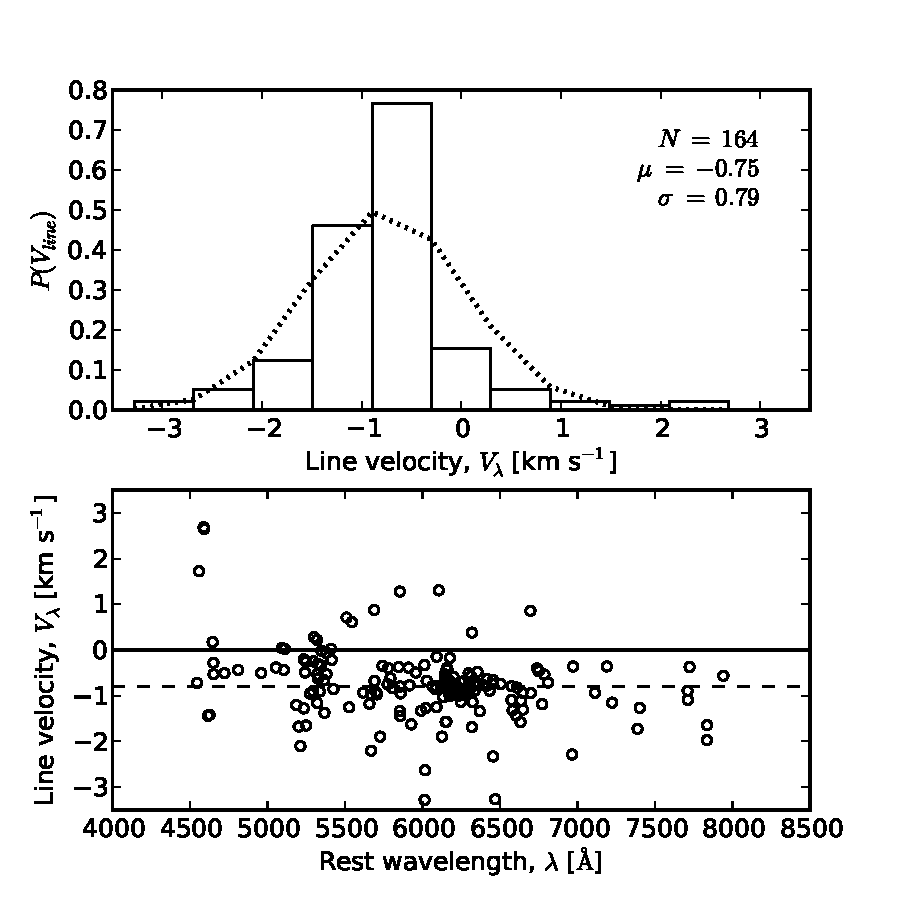
\includegraphics[width=\columnwidth]{./figures/line-velocity.pdf}
%	\caption{Residual velocities for each absorption line with a well-fitted Gaussian profile after correcting for doppler shift using the initial cross-correlation measurement. The mean residual velocity of $-0.75$\,km\,s$^{-1}$ is within the 1-$\sigma$ cross-correlation uncertainty of $\pm0.9$\,km\,s$^{-1}$.}
%	\label{fig:line-velocities}
%\end{figure}



\subsection{Line Measurements}
\label{sec:line-measurements}


\begin{deluxetable*}{clcrccccccc}
\tablecolumns{2}
\tabletypesize{\scriptsize}
\tablecaption{List of Atomic Transitions and Equivalent Width Measurements for Program and Standard Stars \label{tab:equivalent-widths}}
\tablehead{
& & & & & \multicolumn{5}{c}{Equivalent Width} \\
\cline{5-10} \\
Wavelength & Species & $\chi$ & $\log{gf}$ & C222531-145437 & C2306265-085103 & J221821-183424 & J223504-152834 & J223811-104126 & (cont..) \\
({\AA}) & & (eV) & & (m{\AA}) & (m{\AA}) & (m{\AA}) & (m{\AA}) & (m{\AA})
}
\startdata
 6300.30 &  O\,\textsc{i} &      0.00 &    --9.72 &      45.4 &      66.9 &      38.5 &      32.8 &      17.9 \\
 6363.78 &  O\,\textsc{i} &      0.02 &   --10.19 &      19.5 &      28.3 &      13.0 &      18.8 &   \nodata \\
 5688.19 & Na\,\textsc{i} &      2.11 &    --0.42 &   \nodata &   \nodata &      49.0 &     131.5 &      38.4 \\
 6154.23 & Na\,\textsc{i} &      2.10 &    --1.53 &      24.1 &      38.9 &   \nodata &      48.5 &   \nodata \\
 6160.75 & Na\,\textsc{i} &      2.10 &    --1.23 &      37.7 &      58.5 &   \nodata &      65.7 &   \nodata \\
 6318.72 & Mg\,\textsc{i} &      5.11 &    --1.97 &   \nodata &      47.9 &      14.7 &      62.8 &       8.9 \\
 6319.24 & Mg\,\textsc{i} &      5.11 &    --2.22 &      30.8 &   \nodata &       5.5 &   \nodata &   \nodata \\
 6965.41 & Mg\,\textsc{i} &      5.75 &    --1.51 &   \nodata &   \nodata &   \nodata &      59.2 &   \nodata
\enddata
\tablenotetext{}{Table \ref{tab:equivalent-widths} is published in its entirety in the electronic edition. A portion is shown here for guidance regarding its form and content.}
\end{deluxetable*}


For the measurement of atomic absorption lines, we employed the line list of \citet{yong;et-al_2005} with additional transitions of Cr, Sc, Zn, and Sr from \citet{roederer;et-al_2010}. The list has been augmented with molecular CH data from \citet{plez;et-al_2008}. Isotopic and hyperfine splitting data was taken from \citet{citation_needed}. For molecular features (e.g. CH), or lines with hyperfine and/or isotopic splitting (Sc, V, Mn, Co, Cu, Ba, La, Eu), we determined the abundance using spectral synthesis with the relevant data included. For all other transitions, abundances were inferred from curve-of-growth with measured EWs.

The EWs for all absorption lines were measured automatically using software written during this study. The local continuum surrounding every atomic transition is determined, and a Gaussian profile is iteratively fit to the absorption feature of interest. Our algorithm accounts for crowded or blended regions by weighting pixels as a function of difference to the rest wavelength. These algorithms and software will be fully outlined in a future contribution (Casey et al 2013d, in preparation). For this study we have verified our approach by comparing EWs of 156 lines measured by hand and tabulated in \citet{norris;et-al_1996}. We only included measurements in the \citet{norris;et-al_1996} study that were not marked with questionable line quality parameters. Excellent agreement is found between the two studies, which is illustrated in Figure \ref{fig:ew-compare}. The mean difference is a negligible ${-0.64 \pm 2.78}$\,m\AA{}, and no systematic trend is present. The scatter can be attributed to the lack of significant digits in the \citet{norris;et-al_1996} study, as well as the $S/N$ of the data. Other studies \citep[e.g.][]{frebel;et-al_2013} using the same algorithm described here find better agreement for spectra with higher $S/N$ ratios: $0.20 \pm 0.16$\,m{\AA} when we compare our results with manual measurements by \citet{aoki;et-al_2007}, and a difference of $0.25 \pm 0.28$\,m{\AA} is found between manual measurements by \citet{cayrel;et-al_2004} and our automatic results. Although we are extremely confident in our EW measurements, \textit{every} absorption profile was repeatedly examined by eye for quality, and spurious measurements were removed.

\begin{figure}[t]
	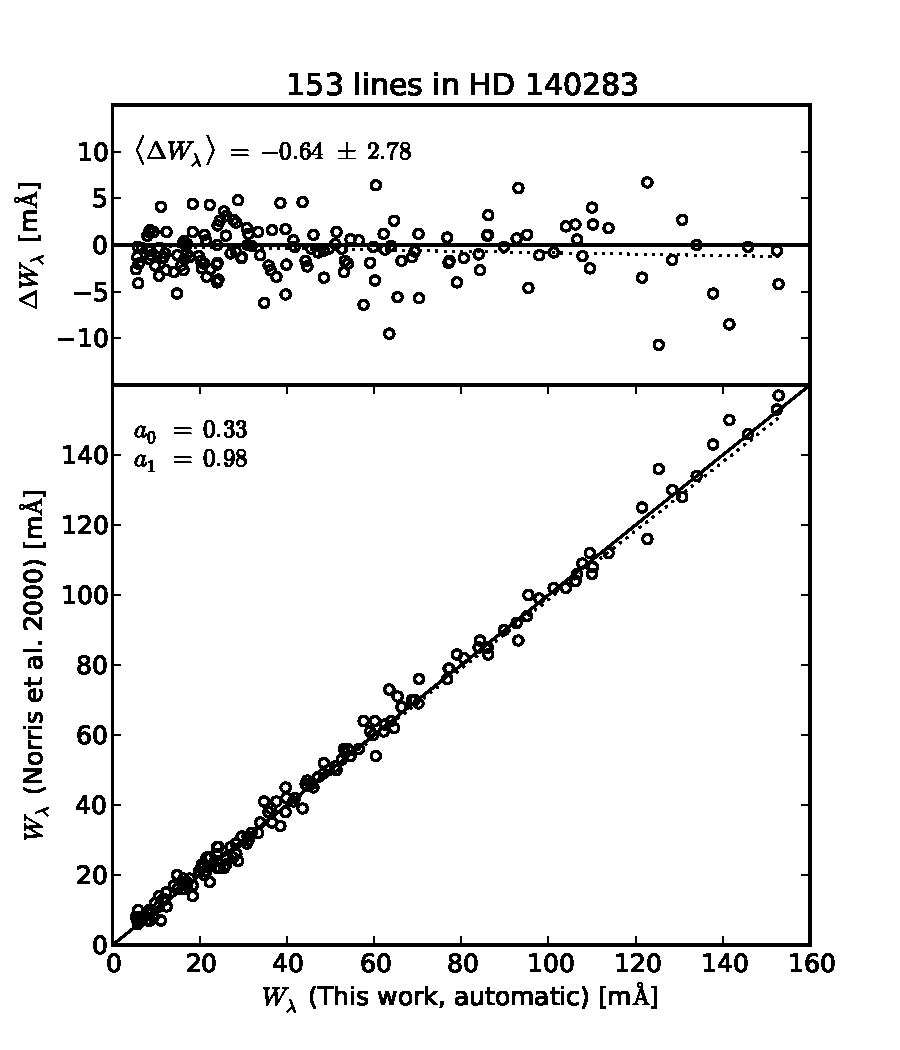
\includegraphics[width=\columnwidth]{./figures/smh-norris.pdf}
	\caption{Comparison showing equivalent widths measured for HD\,140283 using our automatic routine (see \S\ref{sec:line-measurements}), and manual measurements by \citet{norris;et-al_1996}. No systematic trend is present, and the mean difference between these studies is ${\langle\Delta{}W_\lambda\rangle = -0.64 \pm 2.78}$\,m\AA{}.}
	\label{fig:ew-compare}
\end{figure}

We list the atomic data and measured EWs in Table \ref{tab:equivalent-widths}. Transitions near the flat portion of the curve-of-growth have been excluded by removing measurements with reduced equivalent widths (REW), ${\log_{10}{(EW/\lambda)} > -4.5}$. A minimum detectable EW was calculated as a function of wavelength, $S/N$ and spectral resolution by following \citet{norris;et-al_2001}, and only lines that exceeded a 3$\sigma$ detection significance were included for this analysis. 

\subsection{Model Atmospheres}
We have employed the ATLAS9 plane-parallel stellar atmospheres of \citet{castelli;kurucz_2003}. These one-dimensional models ignore any centre-to-limb spatial variations, assume hydrostatic equilibrium and no convective overshoot from the photosphere. The stellar parameter spacing between models is 250\,K in temperature, 0.5\,dex in surface gravity, 0.5\,dex in [M/H] and 0.1\,dex in [$\alpha$/Fe]. We interpolated the temperature, gas and radiative pressure, electron density and opacities between atmosphere models using the Quickhull algorithm \citep{barber;et-al_1996}. Quickhull is reliant on Delaunay tessellation, which suffers from extremely skewed cells when the grid points vary in size by orders of magnitude -- as $T_{\rm eff}$ values do compared to $\log{g}$ or [(M,$\alpha$)/H]. If unaccounted for, performing interpolation using such asymmetric cells can result in significant errors in atmospheric properties across all photospheric depths. We scaled each stellar parameter between zero and unity before interpolation to minimise these interpolation errors. 

%HD\,136316 % F giant, -1.8, Gratton 2000+, has Na, O abundances [DONE]
%HD\,141531 % F giant, -1.6, Gratton 2000+, has Na, O abundances [DONE]
%HD\,44007 % G giant, -1.50, lots of references

\setlength{\tabcolsep}{4pt}

\begin{deluxetable*}{lccccccccccccccc}[h!]
\tablecolumns{2}
\tabletypesize{\tiny}
\tablecaption{Stellar Parameters\label{tab:stellar-parameters}}
\startdata
\hline \\
& \multicolumn{4}{c}{{\bf This Study}} && \multicolumn{5}{c}{{\bf Literature}} \\
\cline{2-5} \cline{7-11} \\

	Designation &
	$T_{\rm eff}$ &
	$\log{g}$ &
	$v_t$ &
	[Fe/H] & 
	&
	$T_{\rm eff}$ &
	$\log{g}$ &
	$v_t$ &
	[Fe/H] &
	Reference \\
	& (K) & (dex) & (km\,s$^{-1}$) & (dex) && (K) & (dex) & (km s$^{-1}$) & (dex) \\
\hline


\\
\multicolumn{11}{c}{Standard Stars} \\
\hline
HD\,41667		& 4660	& 1.71	& 1.84 	& $-$1.20&
				& 4605	& 1.88	& 1.44	& $-$1.16
				& \citet{gratton;et-al_2000} \\
HD\,44007		& 4835	& 1.78	& 1.95	& $-$1.77&
				& 4850	& 2.00 	& 2.20	& $-$1.71
				& \citet{fulbright_2000} \\
HD\,76932		& 5800 & 3.88 & 1.65 & $-$1.05&
				& 5849 & 4.11 & \nodata & $-$0.88 
				& \citet{nissen;et-al_2000} \\
HD\,136316		& 4355 & 0.58 & 2.06 & $-$1.93&
				& 4414 & 0.94 & 1.70 & $-$1.90 
				& \citet{gratton_sneden_1991} \\
HD\,141531		& 4345 & 0.63 & 2.07 & $-$1.69 &
				& 4280 & 0.70 & 1.60 & $-$1.68
				& \citet{shetrone_1996} \\
HD\,142948		& 5025	& 2.25	& 2.05	& $-$0.74&
				& 4713 	& 2.17 	& 1.38	& $-$0.77
				& \citet{gratton;et-al_2000} \\
\hline \\


\multicolumn{11}{c}{Program Stars} \\
\hline 

C222531-145437	& 4365				& 1.25				& 1.94				& $-$1.22	&
				& 4235\,$\pm$\,118 	& 1.45\,$\pm$\,0.21	& 1.96\,$\pm$\,0.11 	& $-$1.20\,$\pm$\,0.14 
				& \citet{wylie-de-boer;et-al_2012} \\
C230626-085103	& 4225	& 0.85	& 1.92 	& $-$1.13&
				& \dots	& \dots	& \dots	& \dots
				& \dots \\	
J221821-183424	& 4630				& 0.88				& 2.16				& $-$1.58&
				& 4395\,$\pm$\,205 	& 1.45\,$\pm$\,0.35 	& 1.96\,$\pm$\,0.18 	& $-$1.15\,$\pm$\,0.21
				& \citet{wylie-de-boer;et-al_2012} \\
J223504-152834	& 4650				& 2.16 				& 1.55				& $-$0.63&
				& 4597\,$\pm$\,158 	& 2.40\,$\pm$\,0.14 	& 1.47\,$\pm$\,0.07 	& $-$0.98\,$\pm$\,0.17
				& \citet{wylie-de-boer;et-al_2012} \\
J223811-104126	& 5190				& 2.93				& 1.62				& $-$1.43&
				& 5646\,$\pm$\,147 	& 4.60\,$\pm$\,0.15 	& 1.09\,$\pm$\,0.11 	& $-$1.20\,$\pm$\,0.20
				& \citet{wylie-de-boer;et-al_2012} 
\enddata

\end{deluxetable*}



\subsection{Stellar Parameters}
The May 2011 version of the \textsc{moog}  \citep{sneden;et-al_1973} spectral synthesis code has been used to derive individual line abundances and stellar parameters. This version employs Rayleigh scattering \citep{sobeck;et-al_2011} instead of treating scattering as true absorption, which is particularly important for transitions blue-ward of 450\,nm. This is noteworthy, but is less relevant for these analyses as most of the atomic transitions utilised here are red-ward of 450\,nm. 





\subsubsection{Effective Temperature}
\label{sec:effective-teffs}
The effective temperature, $T_{\rm eff}$, for each star was found by demanding a zero-trend in excitation potential and line abundance for measurable Fe\,\textsc{i} transitions. The data were fitted with a linear slope, and gradients less than $|10^{-3}|$\,dex eV$^{-1}$ were considered to be converged. For comparison, photometric temperatures were calculated after our spectroscopic temperatures had been derived, and these are discussed in Section \ref{sec:photometric-temperatures}.

\subsubsection{Microturbulence and Surface Gravity}
The microturbulence for each star was found by forcing a zero-trend in the REW and abundance for Fe\,\textsc{i} lines. Similar to the effective temperature, linear slopes in REW and abundance of less than $|10^{-3}|$\,dex were considered converged. The surface gravity for all stars was found by forcing the mean Fe\,\textsc{i} and Fe\,\textsc{ii} abundances to be equal. The process is iterative: a zero trend with the excitation potential, REW and  abundances must be maintained.

\subsubsection{Metallicity}
The model atmosphere metallicity was exactly matched to that of our mean Fe\,\textsc{i} abundance. Individual Fe line abundances that were unusually deviant (e.g. $>$3$\sigma$) from the mean abundance were removed. The largest number of outlier measurements removed for any observation was nine for C222531-145437. These were transitions near the flat part of the curve-of-growth with REWs $\sim -4.5$, leaving 60 Fe\,\textsc{i} and 10 Fe\,\textsc{ii} lines for the analysis of C222531-145437. Usually only one outlier measurement was removed for the other candidates. The minimum number of Fe transitions employed for stellar parameter determination was 42 lines (33 Fe\,\textsc{i} and 9 Fe\,\textsc{ii}), which occurred for our hottest star, J223811-104126.

\subsubsection{Photometric Effective Temperatures}
\label{sec:photometric-temperatures}
 
As a consistency check for our spectroscopic temperatures, we have estimated effective temperatures using the colour-$T_{\rm eff}$ empirical relationship for giant stars from \citet{ramirez;melendez_2005}. The $V-K$ colour has been employed as its calibration has the lowest residual fit. This relationship has a slight dependence on metallicity, and as such we have adopted the spectroscopic [Fe/H] values in Table \ref{tab:stellar-parameters} for these calculations. Optical $V$-band photometry has been sourced from the APASS catalogue \citep{henden;et-al_2012}, and $K$-band magnitudes have been sourced from the 2MASS catalog \citep{skrutskie;et-al_2006}. The reddening maps of \citet{schlegel;et-al_1998} estimate that the extinction for our stars varies between ${E(B-V) = 0.03}$ to {0.07\,mags}, and these values have been used to de-redden our $V-K$ colour.

\setlength{\tabcolsep}{4pt}
\begin{deluxetable}{lccccccc}
\tablecolumns{1}
\tabletypesize{\scriptsize}

\tablecaption{Reddening \& Photometric Temperatures\label{tab:photometric-temperatures}}
\tablehead{
	\colhead{Designation} &
	\colhead{$E(B-V)$} &
	\colhead{$(V-K)_0$} &
	\colhead{$T_{\rm phot}$} &
	\colhead{$T_{\rm spec}$} &
	\colhead{$\Delta{}T$} \\
	& (mag) & (mag) & (K) & (K) & (K)
}
\startdata 
C222531-145437 	& 0.03\phn	& 	2.86 & 4285	& 4365 & $-$80 \\	
C230626-085103	& 0.05\phn	&	3.00 & 4196	& 4225 & $-$29 \\	
J221821-183424 	& 0.03\phn	&	2.36 & 4685	& 4630 &   +55  \\	
J223504-152834 	& 0.04\phn	&	2.50 & 4557	& 4650 & $-$93 \\	
J223811-104126 	& 0.07\phn	&	1.84 & 5240	& 5190 &   +50  
\enddata
\end{deluxetable}
\setlength{\tabcolsep}{6pt}

Calculated photometric temperatures are listed in Table \ref{tab:photometric-temperatures}. The mean difference between the photometric temperatures and those found by excitation balance is $-$19\,K, where the largest variation is $-$93\,K for J223504-152834. While these photometric temperatures serve as a confirmation for our spectroscopically-derived values, for the remainder of this analysis we have employed effective temperatures determined by excitation balance.





% C2225316-145437
% (V-K) = 2.94, V = 12.51, K = 9.57, E(B-V) = 0.03
% (V-K)_0 = 2.86
% with [Fe/H] = -1.22, Ramirez & Melendez Teff: 4285 K (-80 K)

% C230626-085103
% (V-K) = 3.13, V = 12.601, K = 9.47, E(B-V) = 0.05
% (V-K)_0 = 3.00
% with [Fe/H] = -1.13, Ramirez & Melendez Teff: 4196 K (-29 K)

% J221821-183424
% (V-K) = 12.116 - 9.68 = 2.436, E(B-V) = 0.03
% (V-K)_0 = 2.355
% with [Fe/H] = -1.58, Ramirez & Melendez Teff: 4685 (+55 K)

%J223504-152834
% (V-K) = 12.26 - 9.65 = 2.61, E(B-V) = 0.04
% (V-K)_0 = 2.502 
% with [Fe/H] = -0.63, Ramirez & Melendez Teff: 4557 (-93 K)

% J223811-104126
	% (V-K) = 11.933 - 9.90 = 2.033, E(B-V) = 0.07
	% (V-K)0 = 1.844
	% WITH [FE/H] = -1.63 (WRONG), Ramirez & Melendez Teff: 5245 (+55 K)
	% WITH [Fe/H] = -1.43, R & M Teff: 5240 (+50K)

	% (V-K) = 2.033, E(B-V) = 0.12
	% V0 = 11.933 - 0.12 * 3.315
	% K0 = 9.90 - 0.12 * 0.367 
	% (V0 - K0) = 1.67924
	% (V-K)0 = 1.709
	% with [Fe/H] = -1.63 (WRONG), Ramirez & Melendez Teff: 5427 (+237 K)
	% with [Fe/H] = -1.43, R & M Teff = 5423 (+234 K)


\begin{figure*}[t!]
	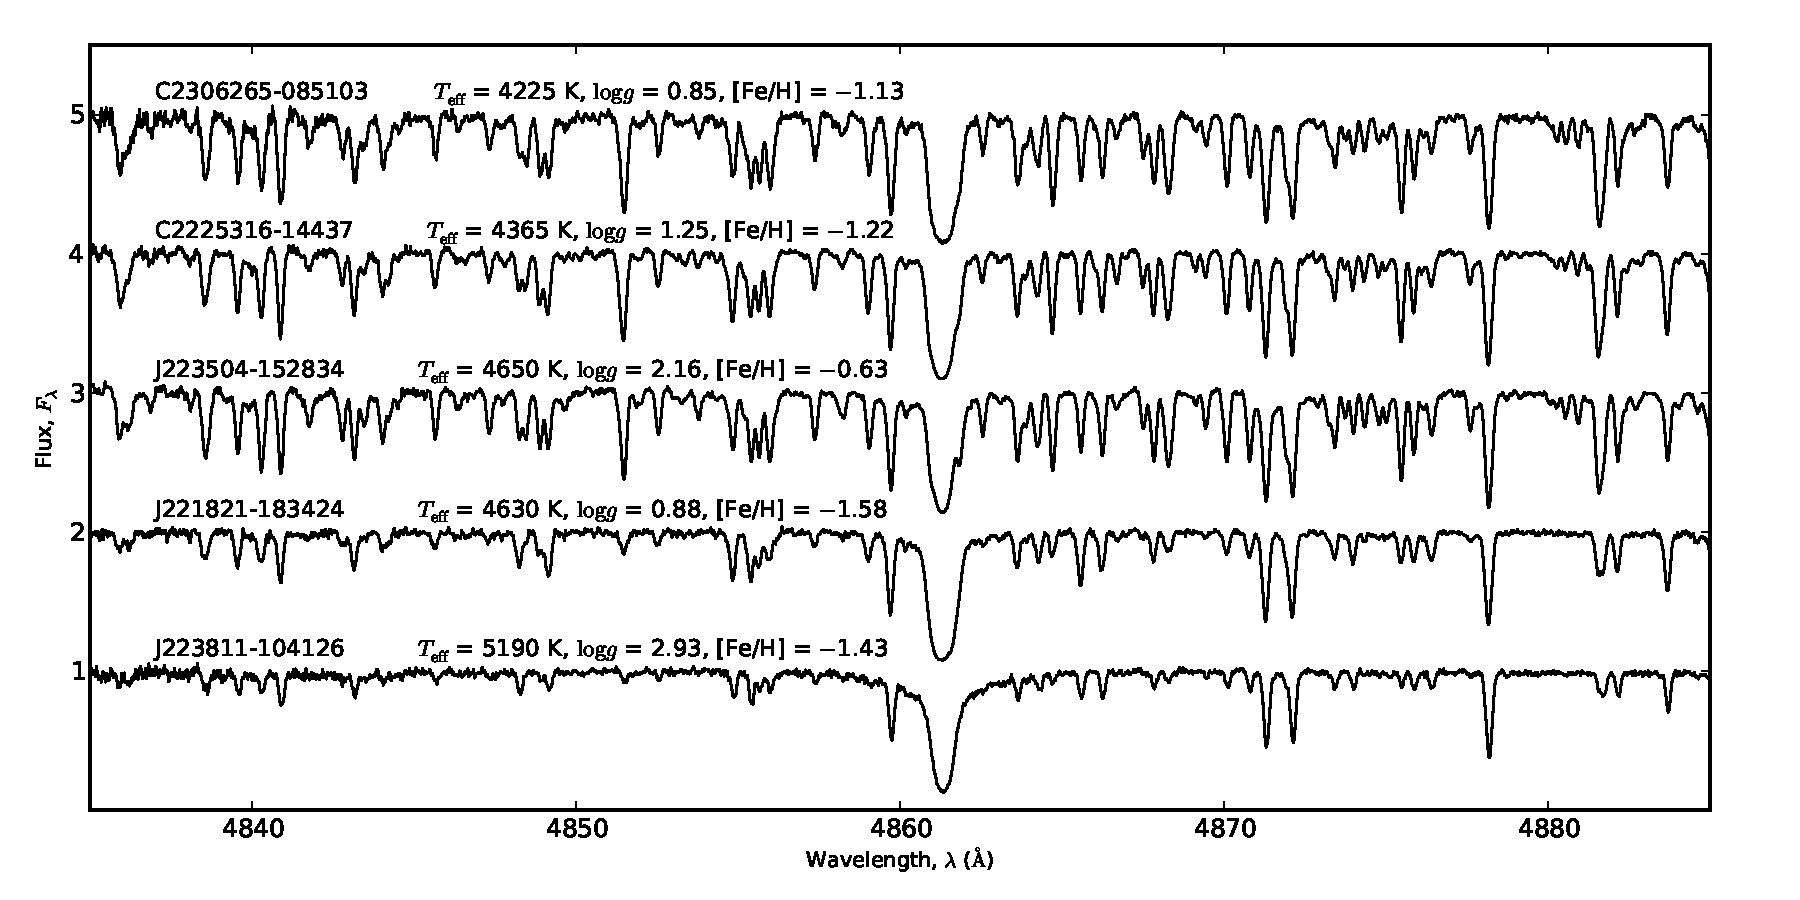
\includegraphics[width=\textwidth]{./figures/spectra-sample.pdf}
	\caption{Normalised rest-frame spectra surrounding the H-$\beta$ absorption line for all Aquarius stream candidates with offset fluxes. The effective temperature, surface gravity and metallicity is shown for all stars.}
	\label{fig:spectra}
\end{figure*}










\subsection{Distances}
\label{sec:distances}

\begin{deluxetable*}{lccccccccc}
\tablecolumns{2}
\tabletypesize{\scriptsize}
\tablecaption{Parameters and Uncertainties for Monte-Carlo Realisations\label{tab:monte-carlo-data}}
\tablehead{
	\colhead{Designation} &
	\colhead{$T_{\rm eff}$} &
	\colhead{$\log{g}$} &
	\colhead{$J$} &
	\colhead{$E(B-V)$} &
	\colhead{$V_{\rm hel}$} &
	\colhead{$\mu_\alpha$} &
	\colhead{$\mu_\delta$} &
	\colhead{$D$}
	\\
	& (K) & (dex) & (mag) & (mag) & (km s$^{-1}$) & (mas yr$^{-1}$) & (mas yr$^{-1}$) & (kpc) 
}
\startdata 
C222531-145437 & $4365 \pm 125$ & $1.25 \pm 0.20$ & $10.341 \pm 0.022$ & $0.03 \pm 0.01$ & $-156.4 \pm 0.1$ & \phn\phn\,$3.5 \pm 2.1$ & $-14.7 \pm 2.2$ & $5.1^{+1.1}_{-0.8}$\\
C230626-085103 & $4225 \pm 125$ & $0.85 \pm 0.20$ & $10.312 \pm 0.025$ & $0.05 \pm 0.01$ & $-221.1 \pm 0.1$ & \phn$-2.5 \pm 2.8$ & $-15.4 \pm 2.7$ & $6.5^{+1.4}_{-1.1}$\\
J221821-183424 & $4630 \pm 125$ & $0.88 \pm 0.20$ & $10.340 \pm 0.021$ & $0.03 \pm 0.01$ & $-159.5 \pm 0.1$ & $-10.6 \pm 2.5$ & $-19.3 \pm 2.5$ & $5.6^{+1.3}_{-0.9}$ \\
J223504-152834 & $4650 \pm 125$ & $2.16 \pm 0.20$ & $10.363 \pm 0.025$ & $0.04 \pm 0.01$ & $-169.7 \pm 0.1$ & \phn\,$15.9 \pm 2.2$ & $-12.8 \pm 2.2$ & $1.9^{+0.5}_{-0.4}$ \\
J223811-104126 & $5190 \pm 125$ & $2.93 \pm 0.20$ & $10.420 \pm 0.018$ & $0.07 \pm 0.01$ & $-235.7 \pm 0.1$ & $-25.3 \pm 2.1$ & $-99.5 \pm 2.1$ & $1.1^{+0.3}_{-0.2}$
\enddata
\end{deluxetable*}
% TODO - Update distances in above table 

Many groups have determined distances for stars in the RAVE survey catalog, which includes all Aquarius stream members. \citet{williams;et-al_2011} tabulated a range of distances inferred by different techniques. Not every measurement technique was applicable to all Aquarius stars. The reduced proper motion distance technique was the only method to estimate distances for all Aquarius candidates. The variations between distance measurements are large. In particular, the distance for {C222531-146537} ranged from $1.4 \pm 0.1$\,kpc \citep{burnett_binney_2010} to $10.3 \pm 2.4$\,kpc \citep{breddels;et-al_2010}, where both groups claim to have the ``most likely'' distances.

\begin{figure}[h]
	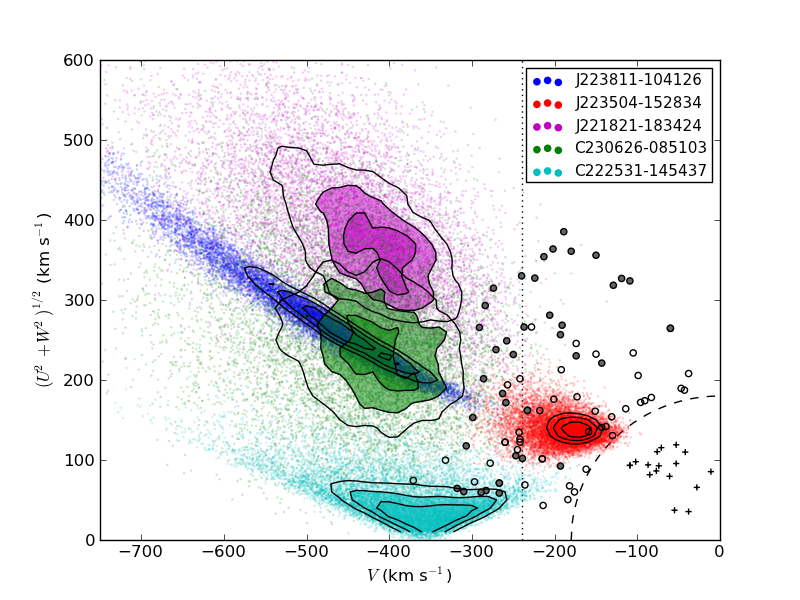
\includegraphics[width=\columnwidth]{./figures/toombre.pdf}
	\caption{Galactic plane rotational velocities versus out-of-plane total velocities. The contours of each star represent the 68\% and 95\% confidence intervals from 10,000 Monte-Carlo realisations of the parameter distributions shown in Table \ref{tab:monte-carlo-data}. A sample of thick disc data from \citet{nissen;schuster_2010} is shown ($+$), as well as their high- and low-alpha halo populations ($\diamond$ and $\circ$ respectively).}
	\label{fig:toombre}
\end{figure}

Using the stellar parameters tabulated in Table \ref{tab:stellar-parameters}, we have calculated distances by isochrone fitting. The \citet{dotter;et-al_2008} $\alpha$-enhanced isochrones were used for these calculations, and an age of 10\,Gyr was assumed for all stars \citep{williams;et-al_2011,wylie-de-boer;et-al_2012}. The closest point to the isochrone was found by taking the uncertainties in $T_{\rm eff}$ and $\log{g}$ (see Section \ref{sec:uncertainties}) into account and measuring the distance modulus in the $J$ band. Given the (i) number of uncertain measurements involved in calculating distances ($T_{\rm eff}$, $\log{g}$, $E(B-V)$, $J$) and (ii) the resultant asymmetric uncertainties, distances were determined from 10,000 Monte-Carlo realisations. Table \ref{tab:monte-carlo-data} lists the input parameters and uncertainties adopted for the Monte-Carlo realisations, as well as the emergent distances and uncertainties. Uncertainties in input parameters were assumed to be normally distributed. Of the distance scales collated in \citet{williams;et-al_2011}, our distances are in most agreement with the \citet{zwitter;et-al_2010} system. In fact, we find the best agreement with the mean of all the distance scales tabulated in \citet{williams;et-al_2011}. The uncertainties in our distance determinations are on the order of twenty per cent.



\subsection{Dynamics}

% U, V, W calculations
Velocity vectors and galactic orbits have been determined in the same Monte-Carlo realisations outlined in Section \ref{sec:distances}, which includes uncertainties in distances, proper motions\footnote{The proper motions in Table 1 of \citet{williams;et-al_2011} are mis-associated to incorrect stars. This error was typographical; it did not affect the transverse velocity calculations (M.E.K. Williams, private communication). The proper motions listed in our Table \ref{tab:monte-carlo-data} are correct.} and heliocentric velocities. We assume no uncertainty in on-sky position $(\alpha, \delta)$. Orbital energy calculations have assumed a three-component (bulge, disc, halo) model of the Galactic potential that reasonably reproduces the Galactic rotation curve. The bulge is represented by a Hernquist potential:

\begin{equation}
	\Phi_{\rm bulge}(x, y, z) = \frac{GM_b}{r + a}
\end{equation}

\noindent where $a = 0.6$\,kpc. The disc is modelled as a Miyamoto-Nagai potential \citep{miyamoto;nagai_1975} where:

\begin{equation}
	\Phi_{\rm disc}(x, y, z) = \frac{GM_{\rm disc}}{\sqrt{x^2 + y^2 + (b + \sqrt{z^2 + c^2})^2}}
\end{equation}

\noindent with $b = 4.5$\,kpc and $c = 0.25$\,kpc and the Galactic halo is represented by a Navarro-Frenk-White dark matter halo \citep{navarro;et-al_1997}:

\begin{equation}
	\Phi_{\rm halo} = -\frac{GM_{\rm vir}}{r\left[\log{(1 + c)} - c/(1 + c)\right]}\log{\left(1 + \frac{r}{r_s}\right)}
\end{equation}

\noindent{}with the three components scaled such that the disc provides 85\% of the radial force at $R_{\rm GC}$, in order to yield a flat circular-speed curve at $R_{\rm GC}$. The solar motion of \citet{schonrich;et-al_2012} has been adopted, where $R_{\rm GC}$ = 8.27\,kpc and a circular velocity speed $V_c = 238$\,km s$^{-1}$.

The Aquarius stream members have bound orbits, all of which are probably retrograde except for {J223504-152834} (Figure \ref{fig:toombre}). Orbital energies and angular momenta from Monte-Carlo simulations are illustrated in Figure \ref{fig:orbits}. The 16,686 stars from the Geneva-Cophenhagen Survey sample \citep{nordstrom;et-al_2004} are also shown as a reference, which primarily consists of nearby disc stars. 


\begin{figure}[h!]
	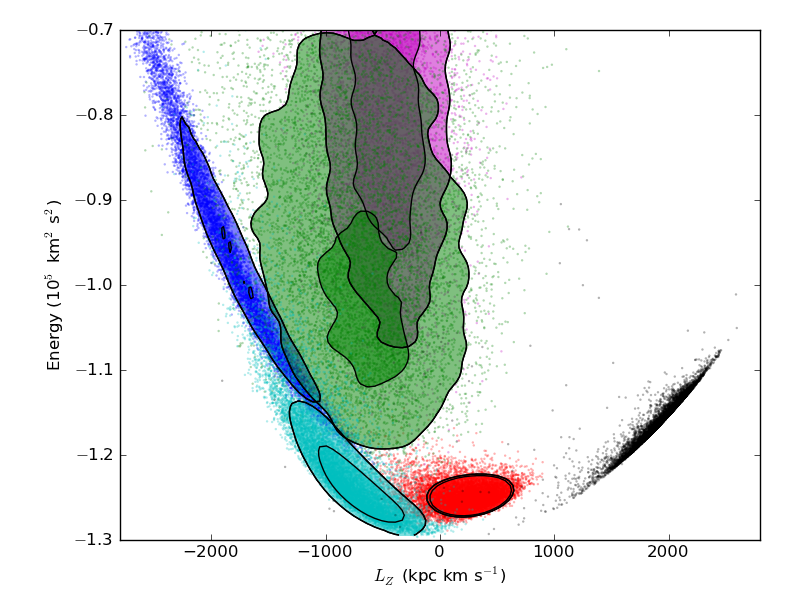
\includegraphics[width=\columnwidth]{./figures/Lz-E.pdf}
	\caption{A Linblad ($L_Z-E$) diagram showing angular momenta and orbital energies after 10,000 Monte-Carlo realisations for each Aquarius stream star. Iso-contours represent the 68\% and 95\% confidence intervals. The black points without contours are from the Geneva-Cophenagen Survey sample \citep{nordstrom;et-al_2004}, which primarily consists of nearby disc stars and serves as a validation of our orbital energy calculations.}
	\label{fig:orbits}
\end{figure}



\section{Chemical Abundances}
\label{sec:chemical-abundances}
We have scaled our chemical abundances to Solar values using the chemical composition described in \citet{asplund;et-al_2009}. The abundances for the standard and program stars are shown in Tables \ref{tab:standard-star-abundances} and \ref{tab:program-star-abundances}, respectively. The discussion of comparable elements are grouped accordingly.

\subsection{Carbon}
Carbon is produced by the triple-$\alpha$ process and ejected through supernovae events, or by mass-loss from asymptotic giant branch (AGB) stars \citep{kobayashi;et-al_2011}. The carbon abundance at the stellar surface increases as the star evolves along the AGB \citep[e.g.,][]{herwig_2005} owing to repeated third dredge-up events. 

%The enriched envelope is then ejected into the interstellar medium by strong stellar winds.

% In particular, the C/O ratio increases, reaching values above unity owing to repeated third dredge-up events. The enriched envelope is then ejected into the interstellar medium through strong stellar winds.

We have measured carbon abundances for all stars from the G-band head near 431.3\,nm and the CH molecular feature at 432.3\,nm, by comparing observed spectra with synthetic spectra for different carbon abundances. The synthetic spectra were convolved with a Gaussian kernel where the width was determined from nearby atomic lines with known abundances. Carbon was measured separately for both features, and in all stars the two measurements agree within 0.10\,dex. An example fit to this spectral region for J223811-104126 is shown in Figure \ref{fig:carbon}.

Carbon abundances in our standard stars agree well with the literature. For HD\,136316 we find {${\rm [C/Fe]} = -0.50 \pm 0.15$}, where \citet{gratton;et-al_2000} find {[C/Fe] $= -0.66$}. Our ${{\rm [C/Fe]} = -0.48}$ measurement for HD\,141531 agrees with \citet{gratton;et-al_2000} to within 0.06\,dex. Most program stars have near-solar carbon abundances, ranging from ${{\rm [C/Fe]} = -0.30}$ for {J221821-183424}, and +0.05 for {J223811-104126}.

\begin{figure}[h!]
	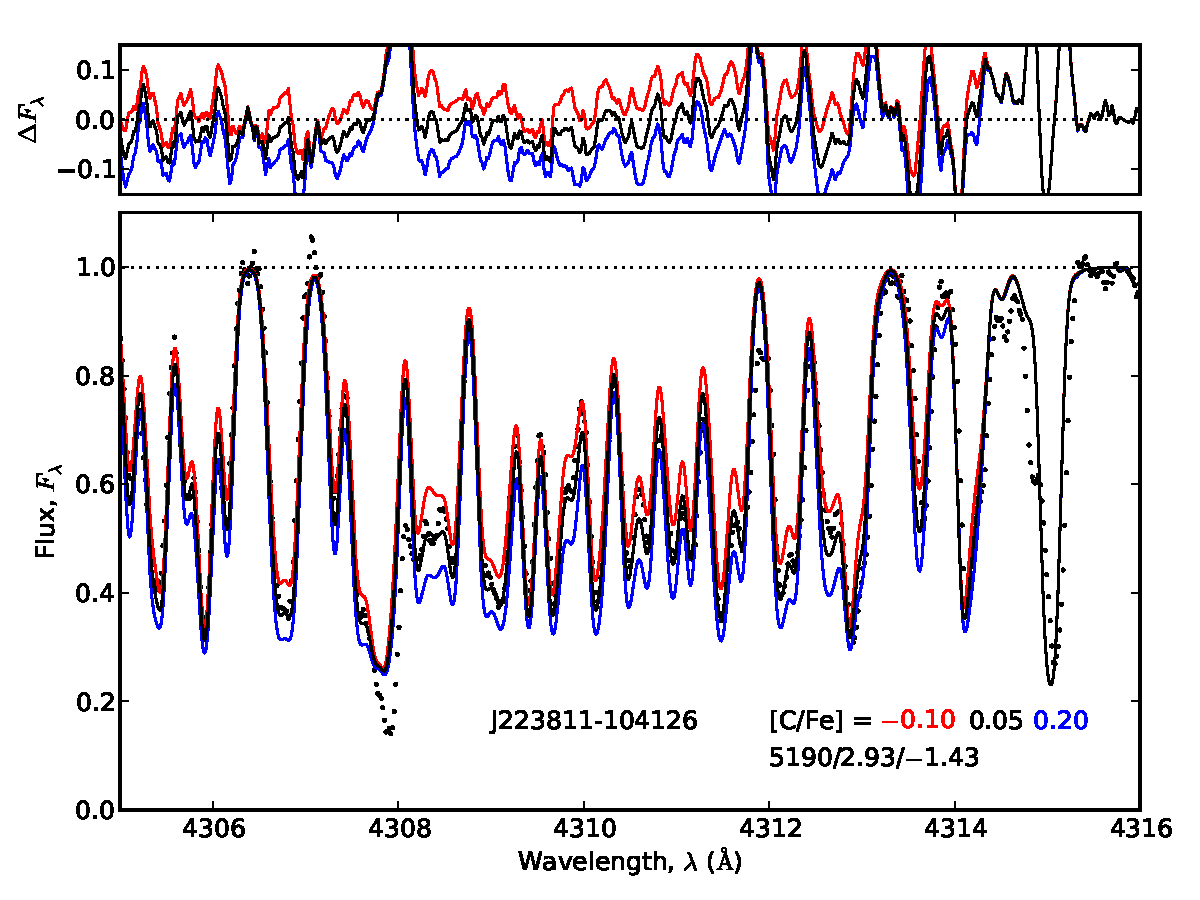
\includegraphics[width=\columnwidth]{./figures/J223811-C.pdf}
	\caption{The carbon CH feature near 4313\,{\AA} in program star J223811-104126. The best-fit synthetic spectra is shown, with synthetic spectra for $\pm0.15$\,dex about the best-fitting abundance.}
	\label{fig:carbon}
\end{figure}


\subsection{Oxygen}
\label{sec:oxygen-abundances}
Oxygen can be a particularly difficult element to measure. There are only a handful of lines available in an optical spectrum: the forbidden {[O\,\textsc{i}]} lines at 630\,nm and 636\,nm, and the O\,\textsc{i} triplet lines at 777\,nm. The forbidden lines are very weak and become difficult to measure in hot and/or metal-poor stars (${\mbox{[Fe/H]} \lesssim -1.5}$\,dex). When they are present, depending on the radial velocity of the star, the {[O\,\textsc{i}]} lines can be significantly affected by telluric absorption. Moreover, the 630\,nm line is blended with a Ni\,\textsc{i} absorption line \citep{allende-prieto;et-al_2001}. Hence the region requires careful consideration. Although the O\,\textsc{i} triplet lines at 777\,nm are stronger than the forbidden lines, they are extremely susceptible to non-LTE effects, surface granulation \citep{asplund;perez_2001}, and are sensitive to changes in microturbulence. Forbidden {[O\,\textsc{i}]} abundances in HD\,136316 agree well with \citet{gratton;et-al_2000}, where a difference of $-0.07$\,dex is observed.

The {[O\,\textsc{i}]} lines were measurable in four of our Aquarius stream candidates. The 630\,nm line in one of our candidates, {C2306265-085103}, was sufficiently affected by telluric absorption such that we deemed the line unrecoverable. Thus, only the 636\,nm transition was used to derive an oxygen abundance for {C2306265-085103}. In our hottest star, {J223811-104126}, the forbidden oxygen lines were not detected above a 3$\sigma$ significance. After synthesising the region, we deduce a very conservative upper limit of ${\mbox{[O/Fe]} < 0.50}$\,dex from the {[O\,\textsc{i}]} lines. This is consistent with the rest of our candidates, with [O/Fe] abundances varying between 0.43 to 0.49\,dex.

In order to derive an oxygen measurement for {J223811-104126}, we were forced to use the triplet lines at 777\,nm. We extended these measurements for all Aquarius stars, and a mean abundance for each candidate was found from the synthesis of the permitted triplet lines. Oxygen abundances inferred from the triplet lines in all other stars were systematically $+0.27$\,dex higher than abundances calculated from the {[O\,\textsc{i}]} forbidden lines. \citet{perez;et-al_2006} found the same result: [O/Fe] values based on the {O\,\textsc{i}} permitted triplet lines are on average ${+0.19 \pm 0.07}$\,dex higher than those found from the forbidden lines, which did not include non-LTE corrections of $+$0.08\,dex. Thus, we attribute our $+$0.27\,dex offset between measurements of the {[O\,\textsc{i}]} and {O \textsc{i}} triplet lines to non-LTE and 3D effects. \citet{perez;et-al_2006} concluded that the forbidden lines, when not too weak, probably give the most reliable estimate of oxygen abundance. From the permitted O\,\textsc{i} triplet in {J223811-104126}, we derive an oxygen abundance of ${\mbox{[O/Fe]} = 0.42 \pm 0.01}$\,dex (random scatter). This measurement will be systematically higher than the `true' abundance if it were discernible from the [O\,\textsc{i}] lines, on the order of ${\sim}+0.27$\,dex. When we apply this crude offset derived from the rest of our sample, we arrive at a corrected abundance of ${\mbox{[O/Fe]} = 0.15 \pm 0.13}$\,dex (total uncertainty) for {J223811-104126}. This is the most oxygen-deficient star in our sample by a factor of two.


\subsection{Sodium and Aluminium}
\label{sec:sodium-abundances}
Our line list includes three clean, unblended sodium lines at 568.8\,nm, 615.4\,nm and 616.1\,nm. Not all three of these lines were detectable in each star. In the hottest and most metal-poor stars, J223811-104126 and J221821-183424 respectively, only the 568.8\,nm line was measurable. For stars where multiple sodium lines were available, the line-to-line scatter is usually around 0.04\,dex with a maximum of 0.09\,dex in HD\,41667. However, in calculating total abundance uncertainties (see Section \ref{sec:chemical-abundance-uncertainties}) we have conservatively assumed a minimum random scatter of $\pm0.10$\,dex for all stars.

% [Na/Fe] measurements in the standard stars? 
Our [Na/Fe] abundances appear systematically higher than values found in the literature, on the order of 0.10\,dex. For HD\,142948 we find {[Na/Fe] = 0.22}, which is +0.10\,dex higher than that found by \citet{gratton;et-al_2000}, and similarly we find HD\,76932 to be +0.10\,dex higher than reported by \citet{fulbright_2000}. \citet{gratton;et-al_2000} also found HD\,136316 to have {[Na/Fe] = $-$0.29}\,dex, where we find {[Na/Fe] = $-0.14$}, yet excellent agreement is found in the stellar parameters in \citet{gratton;et-al_2000} and this study. Different solar compositions employed between this study and earlier work can account for $\sim$0.08\,dex of this effect, leaving the residual difference well within the observational uncertainties. However, it is important to note that the [Na/Fe] abundance ratios presented in this study may be slightly higher compared to previous studies.

There are six aluminium transitions in our optical spectra. The strongest of these lines occur at 394.4\,nm and 396.1\,nm and are visible in all of our stars. However this is a particularly crowded spectral region: the lines fall between the strong Ca H and K lines, with the 396.1\,nm transition clearly located in the wing of the Ca H line. Additionally, the 394.4 and 3961\,nm lines have appreciable departures from the assumption of LTE, resulting in under-estimated abundances by up to $\sim$0.6\,dex \citep{baumueller;gehren_1997}. Instead, we have measured Al abundances from other available transitions: the {Al\,\textsc{i}} lines at 669.6, 669.8, 783.5 and 783.6\,nm. Generally the four {Al\,\textsc{i}} lines are in reasonable agreement with one another, yielding random scatter of less than 0.05\,dex. 

\subsection{$\alpha$-elements (Mg, Si, Ca and Ti)}
\label{sec:alpha-elements}

The $\alpha$-elements (Mg, Si, Ca and Ti) are forged through $\alpha$-particle capture during hydrostatic burning of carbon, neon and silicon. Material enriched in $\alpha$-elements is eventually dispersed into the interstellar medium following Type II core-collapse supernovae (SN). 

Depending on the radial velocity of the star, some magnesium lines were affected by telluric absorption, particularly the 631.8 and 696.5\,nm transitions. Atmospheric absorption was most notable for C222531-145437, where three of the four Mg transitions in our line list suffered some degree of telluric absorption, requiring an attentive correction. Every amended absorption profile was carefully examined, and lines with suspicious profiles were excluded from the final magnesium abundance. All [$\alpha$/Fe] abundance ratios in the standard stars are in excellent agreement with the literature. Typically the difference is 0.01\,dex, with the largest discrepancy of {$\Delta$[Ti/Fe] = +0.13\,dex} for HD\,76932 when compared with \citet{fulbright_2000}.

While \citet{wylie-de-boer;et-al_2012} find almost no scatter {($\pm0.02$\,dex)} in [Mg/Fe] for stars common to both studies, we find {C222531-145437} and {J223504-152834} to be almost {$+0.20$\,dex} higher than the rest of the sample. The reason for this [Mg/Fe] discrepancy is not obvious, given the stellar parameters between the two studies agree well, with the previously discussed exception in metallicity.  Of the {Mg\,\textsc{i}} line profiles measured, only two transitions are common to both line lists: 631.8\,nm and 631.9\,nm. The oscillator strengths differ between studies; in these two lines the $\log{gf}$ differs by $-0.24$ and {$-0.27$\,dex} respectively (our oscillator strengths are lower). This indicates that the difference in oscillator strengths may explain the $\sim{}$0.2\,dex offset in [Mg/Fe] between this study and \citet{wylie-de-boer;et-al_2012}.

% [alpha/Fe]
\begin{figure}[h]
	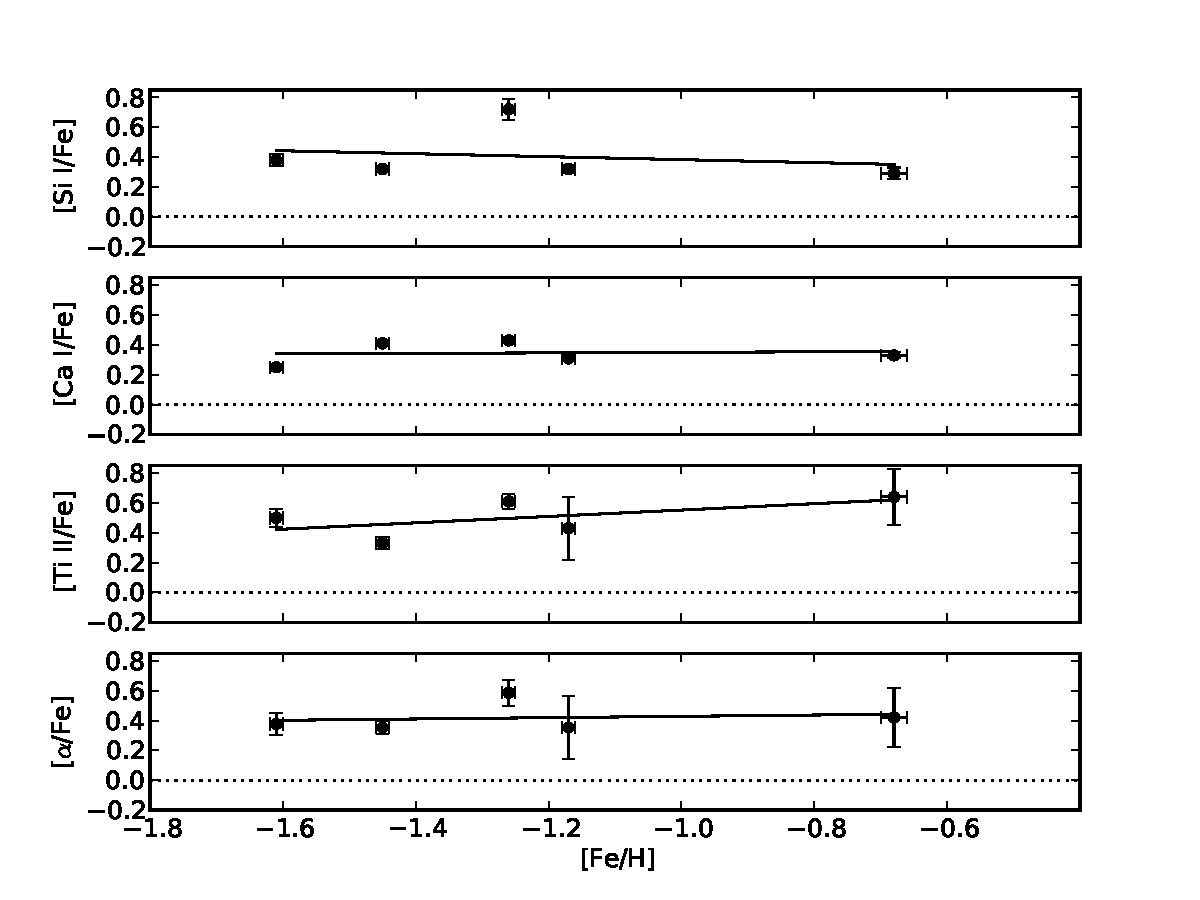
\includegraphics[width=\columnwidth]{./figures/aquarius-alpha-fe.pdf}
	\caption{$\alpha$-element abundances with respect to iron content. The mean [$\alpha$/Fe] abundance from these is shown in the bottom panel. The Solar element-to-iron ratio is shown as a dotted line in each panel.}
	\label{fig:alpha-elements}
\end{figure}

% calcium measurements + silicon measurements
Of all the $\alpha$-elements, calcium has the smallest measurement scatter in our stars. The mean was formed from four line measurements in each star, with a typical random scatter of 0.01\,dex. Nevertheless, the aforementioned conservative minimum of 0.10\,dex for random scatter applies, and uncertainties in stellar parameters will contribute to the total error budget. As shown in Figure \ref{fig:alpha-elements}, all Aquarius stream candidates show super-solar [Ca/Fe], ranging between +0.23 to +0.43\,dex, consistent with [(Mg,Si,Ti)/Fe] measurements. 

{C222531-145437} has an unusually high silicon abundance (${\mbox{[Si/Fe]} = 0.79}$), well outside the uncertainties of the rest of our sample. The 5 silicon line abundances in this star are in relatively good agreement with each another. If we exclude the highest measurement, then the mean abundance drops only slightly to ${\mbox{[Si/Fe]} = 0.73 \pm 0.04}$ (random scatter). The lowest silicon line abundance for {C222531-145437} is ${\mbox{[Si/Fe]} = 0.61}$, which is still significantly higher than the mean abundance for any other star.

% titanium measurements?
Titanium abundance ratios for the stream show typical levels of $\alpha$-enhancement. Our mean titanium abundances are derived from four to seven clean, unblended lines. In our hottest and most metal-poor stars, no suitable Ti\,\textsc{i} transitions were available. 

%In other Aquarius members, the mean difference between species is ${\langle{\rm Ti}\,\textsc{i} - {\rm Ti}\,\textsc{ii}\rangle = 0.24\,{\rm dex}}$. Although this discrepancy in Ti is non-negligible, it is reassuring to find our mean ${\langle{\rm Cr}\,\textsc{i} - {\rm Cr}\,\textsc{ii}\rangle}$ differences are very small (see Section \ref{sec:fe-peak-abundances}).

\subsection{Iron-peak Elements}
\label{sec:fe-peak-abundances}

The Fe-peak elements (Sc to Zn) are primarily synthesized by the explosive nucleosynthesis of oxygen, neon, and silicon burning. Ignition can occur from Type II SN explosions of massive stars, or once a white dwarf accretes enough material to exceed the Chandrasekhar mass limit and spontaneously ignite carbon, leading to a Type Ia SN. 

% The exception here is Cr, where we find a median {$\mbox{[Cr/Fe]} = -0.08 \pm 0.12$} with minimal variation across all [Fe/H], similar to that observed by \citet{reddy;et-al_2006} in the Milky Way.
Although not all {Fe-peak} elements are created equally, the Fe-peak elements generally exhibit similar trends with overall metallicity. All exhibit a positive trend with increasing iron abundance, with varying slope strengths.

The [Sc/Fe] measurements presented in Figure \ref{fig:fe-peak-elements} are averaged from six clean {Sc\,\textsc{ii}} lines, and there is very little line-to-line scatter, the largest of which is {0.06\,dex}. The number of clean, suitable {Cr\,\textsc{i}} lines available between members fluctuated from three to twelve. Very little line-to-line scatter is present in both {Cr\,\textsc{i}} and Cr\,\textsc{ii}: the random scatter is below {0.04\,dex} for most stars. Chromium abundances are only available for one of the standard stars, where our {[Cr/Fe] = 0.03} is in excellent agreement with \citet{fulbright_2000}, where they find {[Cr/Fe] = 0.04}.

% The {Cr\,\textsc{i}} and \textsc{ii} mean abundances for {J223504-152834} are in good agreement (0.05\,dex), and since none of the fitted Gaussian profiles appeared unusual, we chose not to exclude any measurements. For all other stars, the ${\langle{\rm Cr}\,\textsc{i} - {\rm Cr}\,\textsc{ii}\rangle}$ abundance differences varied between {0.02\,dex} up to {0.31\,dex}. The largest discrepancy occurred in our hottest star, where fewer Cr\,\textsc{i} and Cr\,\textsc{ii} transitions were measurable. 

Manganese demonstrates a strong trend with increasing iron abundance (Figure \ref{fig:fe-peak-elements}). A significant source of Mn comes from Type Ia SN, and the strong Mn-Fe trend is consistent with chemodynamical simulations \citep{kobayashi;nakasato_2011}, as well as thick disc observations by \citet{reddy;et-al_2006}.  Although Mn is known to demonstrate significant departures from LTE, we have not applied any non-LTE corrections to our abundances. 


Abundances of Co\,\textsc{i} lines were calculated by synthesis, as they demonstrate appreciable broadening due to hyperfine structure. Although they are known to suffer significant departures from LTE \citep{bergemann;et-al_2010}, no corrections have been made for these data. In general, [Co/H] follows [Fe/H] in our candidates. 
Cu abundances have also been determined by synthesis, and exhibit a strong positive relationship with increasing overall metallicity, consistent with MW trend???

% [TODO] Is Cu/Fe consistent with MW trend?  

Most Aquarius stream stars have seven clean {Ni\,\textsc{i}} transitions available. These lines are in excellent agreement, with a typical scatter of {0.03\,dex}. Nickel abundances have been published for two of our standard stars: HD\,76932 \citep{fulbright_2000} and HD\,141531 \citep{shetrone_1996}. In both cases, our [Ni/Fe] abundance ratios are slightly higher by +0.08 and +0.10\,dex respectively. The different solar compositions employed by these studies can only accounts for 0.01\,dex of this discrepancy, and the differences in oscillator strengths for common Ni\,\textsc{i} lines are negligible. Overall, the [Ni/Fe] abundance ratios in the Aquarius stream stars do not deviate greatly from the Solar ratio.


% Lines commented out in this table are those abundances measured by EWs,
% before synthesis was done with hyperfine structure and isotopic splitting data.
\begin{longtable*}[T]{lcccccclccccccc}
\caption{\\ Standard Star Abundances\label{tab:standard-star-abundances}} \tabularnewline
\cline{1-13}
Species & $N$ & $\log\epsilon(X)$ & $\sigma_\epsilon$ & [X/H] & [X/Fe] &&% $\sigma$ && 
Species & $N$ & $\log\epsilon(X)$ & $\sigma_\epsilon$ & [X/H] & [X/Fe] \tabularnewline %& $\sigma$ \tabularnewline
\cline{1-13} \tabularnewline
% This works.
\endhead
\hline
\multicolumn{13}{r}{Continued..}
\endfoot
\hline
\endlastfoot

\\
\multicolumn{6}{c}{HD\,41667} & \colhead{} & \multicolumn{6}{c}{HD\,44007} \\
\cline{1-6} \cline{8-13}

   C (CH)       &   2 &    6.95 &    0.20 &  --1.48 &  --0.28 && %    0.20 &&
   C (CH)       &   2 &    6.66 &    0.20 &  --1.77 &  --0.01 \\ % &    0.20 \\
   O \textsc{I} &   2 &    7.95 &    0.06 &  --0.74 &    0.46 && %    0.04 &&
   O \textsc{I} &   1 &    7.41 &    0.00 &  --1.28 &    0.48 \\ % &    0.00 \\
  Na \textsc{I} &   3 &    4.90 &    0.18 &  --1.34 &  --0.14 && %    0.10 &&
  Na \textsc{I} &   2 &    4.44 &    0.09 &  --1.80 &  --0.04 \\ % &    0.06 \\
  Mg \textsc{I} &   4 &    6.72 &    0.10 &  --0.88 &    0.32 && %    0.05 &&
  Mg \textsc{I} &   2 &    6.30 &    0.06 &  --1.29 &    0.47 \\ % &    0.04 \\
  Al \textsc{I} &   4 &    5.18 &    0.11 &  --1.27 &  --0.07 && %    0.06 &&
  Al \textsc{I} &   1 &    4.80 & \nodata &  --1.65 &    0.11 \\ % & \nodata \\
  Si \textsc{I} &   5 &    6.55 &    0.06 &  --0.96 &    0.24 && %    0.03 &&
  Si \textsc{I} &   5 &    6.07 &    0.07 &  --1.44 &    0.32 \\ % &    0.03 \\
   K \textsc{I} &   1 &    4.64 & \nodata &  --0.39 &    0.81 && % \nodata &&
   K \textsc{I} &   1 &    4.31 & \nodata &  --0.72 &    1.04 \\ % & \nodata \\
  Ca \textsc{I} &   4 &    5.47 &    0.06 &  --0.87 &    0.33 && %    0.03 &&
  Ca \textsc{I} &   4 &    4.95 &    0.02 &  --1.39 &    0.37 \\ % &    0.01 \\
 Sc \textsc{II} &   5 &    2.00 &    0.12 &  --1.15 &    0.05 && %    0.05 &&
 Sc \textsc{II} &   5 &    1.32 &    0.12 &  --1.85 &  --0.07 \\ % &    0.05 \\
%Sc \textsc{II} &   6 &    2.13 &    0.13 &  --1.02 &    0.18 && %    0.05 &&
%Sc \textsc{II} &   6 &    1.39 &    0.10 &  --1.76 &    0.00 \\ % &    0.04 \\
  Ti \textsc{I} &   4 &    3.96 &    0.04 &  --0.99 &    0.21 && %    0.02 &&
  Ti \textsc{I} &   1 &    3.48 & \nodata &  --1.47 &    0.29 \\ % & \nodata \\
 Ti \textsc{II} &   3 &    4.09 &    0.25 &  --0.86 &    0.35 && %    0.14 &&
 Ti \textsc{II} &   4 &    3.47 &    0.15 &  --1.48 &    0.28 \\ % &    0.07 \\
   V \textsc{I} &   4 &    2.85 &    0.11 &  --1.08 &    0.12 && %    0.05 &&
   V \textsc{I} &   1 &    2.22 & \nodata &  --1.72 &    0.05 \\ % & \nodata \\
%  V \textsc{I} &   6 &    2.87 &    0.13 &  --1.06 &    0.14 && %    0.05 &&
%  V \textsc{I} &   4 &    2.17 &    0.03 &  --1.77 &  --0.00 \\ % &    0.01 \\
  Cr \textsc{I} &  10 &    4.22 &    0.08 &  --1.42 &  --0.22 && %    0.03 &&
  Cr \textsc{I} &  15 &    3.65 &    0.07 &  --1.99 &  --0.22 \\ % &    0.02 \\
 Cr \textsc{II} &   2 &    4.54 &    0.05 &  --1.09 &    0.11 && %    0.04 &&
 Cr \textsc{II} &   3 &    4.00 &    0.01 &  --1.64 &    0.12 \\ % &    0.01 \\
 Mn \textsc{I}  &   3 &    3.87 &    0.04 &  --1.56 &  --0.36 && %    0.03 &&
 Mn \textsc{I}  &   2 &    3.21 &    0.06 &  --2.22 &  --0.48 \\ % &    0.04 \\
% Mn \textsc{I} &   3 &    3.96 &    0.01 &  --1.47 &  --0.27 && %    0.01 &&
% Mn \textsc{I} &   3 &    3.15 &    0.04 &  --2.28 &  --0.52 \\ % &    0.02 \\
  Fe \textsc{I} &  61 &    6.30 &    0.12 &  --1.20 &    0.00 && %    0.02 &&
  Fe \textsc{I} &  51 &    5.74 &    0.13 &  --1.76 &    0.00 \\ % &    0.02 \\
 Fe \textsc{II} &  13 &    6.35 &    0.05 &  --1.15 &    0.05 && %    0.01 &&
 Fe \textsc{II} &  15 &    5.74 &    0.10 &  --1.76 &  --0.00 \\ % &    0.03 \\
  Co \textsc{I} &   3 &    3.73 &    0.06 &  --1.26 &  --0.06 && %    0.03 &&
  Co \textsc{I} &   0 & \nodata & \nodata & \nodata & \nodata \\ % & \nodata \\
% Co \textsc{I} &   5 &    3.75 &    0.10 &  --1.24 &  --0.04 && %    0.04 &&
% Co \textsc{I} &   1 &    3.22 &    0.00 &  --1.77 &  --0.01 \\ % &    0.00 \\
  Ni \textsc{I} &   7 &    4.94 &    0.12 &  --1.28 &  --0.08 && %    0.05 &&
  Ni \textsc{I} &   4 &    4.47 &    0.05 &  --1.75 &    0.01 \\ % &    0.02 \\
  Cu \textsc{I} &   1 &    2.29 & \nodata &  --1.90 &  --0.70 && % \nodata &&
  Cu \textsc{I} &   1 &    1.58 & \nodata &  --2.61 &  --0.85 \\ % & \nodata \\
% Cu \textsc{I} &   1 &    2.72 &    0.00 &  --1.47 &  --0.27 && %    0.00 &&
% Cu \textsc{I} &   1 &    1.84 &    0.00 &  --2.35 &  --0.59 \\ % &    0.00 \\
  Zn \textsc{I} &   2 &    3.36 &    0.08 &  --1.20 &    0.00 && %    0.06 &&
  Zn \textsc{I} &   2 &    2.83 &    0.05 &  --1.73 &    0.03 \\ % &    0.04 \\
  Sr \textsc{I} &   1 &    1.31 & \nodata &  --1.56 &  --0.36 && % \nodata &&
  Sr \textsc{I} &   1 &    0.91 & \nodata &  --1.96 &  --0.20 \\ % & \nodata \\
  Y \textsc{II} &   5 &    0.97 &    0.19 &  --1.24 &  --0.04 && %    0.09 &&
  Y \textsc{II} &   6 &    0.28 &    0.11 &  --1.93 &  --0.16 \\ % &    0.05 \\
  Zr \textsc{I} &   2 &    1.42 &    0.05 &  --1.17 &    0.04 && %    0.04 &&
  Zr \textsc{I} &   0 & \nodata & \nodata & \nodata & \nodata \\ % & \nodata \\
 Zr \textsc{II} &   1 &    1.28 & \nodata &  --1.30 &  --0.10 && % \nodata &&
 Zr \textsc{II} &   1 &    0.59 & \nodata &  --1.99 &  --0.23 \\ % & \nodata \\
 Ba \textsc{II} &   2 &    0.95 &    0.07 &  --1.23 &  --0.02 && %    0.05 &&
 Ba \textsc{II} &   2 &    0.31 &    0.06 &  --1.87 &  --0.11 \\ % &    0.04 \\
%Ba \textsc{II} &   2 &    1.02 &    0.04 &  --1.16 &    0.05 && %    0.02 &&
%Ba \textsc{II} &   2 &    0.25 &    0.01 &  --1.93 &  --0.17 \\ % &    0.01 \\
 La \textsc{II} &   1 &    0.17 & \nodata &  --0.93 &     0.27 && % \nodata &&
 La \textsc{II} &   2 &  --0.57 &    0.05 &  --1.67 &     0.09 \\ % &    0.03 \\
%La \textsc{II} &   2 &    0.14 &    0.04 &  --0.96 &    0.24 && %    0.03 &&
%La \textsc{II} &   2 &  --0.52 &    0.02 &  --1.62 &    0.14 \\ % &    0.01 \\
 Ce \textsc{II} &   4 &    0.35 &    0.18 &  --1.23 &  --0.02 && %    0.09 &&
 Ce \textsc{II} &   3 &  --0.41 &    0.12 &  --1.99 &  --0.23 \\ % &    0.07 \\
 Nd \textsc{II} &   9 &    0.54 &    0.10 &  --0.88 &    0.32 && %    0.03 &&
 Nd \textsc{II} &   9 &  --0.36 &    0.11 &  --1.78 &  --0.01 \\ % &    0.04 \\
 Eu \textsc{II} &   1 &  --0.13 & \nodata &  --0.65 &    0.55 && % \nodata &&
 Eu \textsc{II} &   1 &  --1.16 & \nodata &  --1.68 &    0.08 \\ % & \nodata \\
%Eu \textsc{II} &   1 &  --0.05 &    0.00 &  --0.57 &    0.63 && %    0.00 &&
%Eu \textsc{II} &   1 &  --0.36 &    0.00 &  --0.88 &    0.88 \\ % &    0.00 \\

\cline{1-6} \cline{8-13} \\ \\
\multicolumn{6}{c}{HD\,76932} && \multicolumn{6}{c}{HD\,136316} \\
\cline{1-6} \cline{8-13}
   C (CH)       &   2 &    7.52 &    0.20 &  --0.91 &    0.14 && %    0.20 &&
   C (CH)       &   2 &    5.95 &    0.20 &  --2.48 &  --0.50 \\ % &    0.20 \\
   O \textsc{I} &   0 & \nodata & \nodata & \nodata & \nodata && % \nodata &&
   O \textsc{I} &   1 &    7.17 & \nodata &  --1.52 &    0.41 \\ % & \nodata \\
  Na \textsc{I} &   3 &    5.37 &    0.04 &  --0.87 &    0.18 && %    0.02 &&
  Na \textsc{I} &   2 &    4.17 &    0.04 &  --2.08 &  --0.14 \\ % &    0.02 \\
  Mg \textsc{I} &   3 &    6.95 &    0.20 &  --0.65 &    0.40 && %    0.11 &&
  Mg \textsc{I} &   2 &    6.08 &    0.24 &  --1.52 &    0.41 \\ % &    0.17 \\
  Al \textsc{I} &   4 &    5.45 &    0.07 &  --1.00 &    0.05 && %    0.03 &&
  Al \textsc{I} &   0 & \nodata & \nodata & \nodata & \nodata \\ % & \nodata \\
  Si \textsc{I} &   5 &    6.79 &    0.06 &  --0.72 &    0.33 && %    0.03 &&
  Si \textsc{I} &   4 &    5.89 &    0.05 &  --1.62 &    0.31 \\ % &    0.03 \\
   K \textsc{I} &   1 &    4.94 & \nodata &  --0.09 &    0.96 && % \nodata &&
   K \textsc{I} &   1 &    3.91 & \nodata &  --1.12 &    0.81 \\ % & \nodata \\
  Ca \textsc{I} &   4 &    5.60 &    0.02 &  --0.74 &    0.31 && %    0.01 &&
  Ca \textsc{I} &   4 &    4.71 &    0.02 &  --1.63 &    0.30 \\ % &    0.01 \\
 Sc \textsc{II} &   4 &    2.10 &    0.05 &  --1.05 &    0.01 && %    0.03 &&
 Sc \textsc{II} &   4 &    1.20 &    0.08 &  --1.95 &  --0.02 \\ % &    0.04 \\
%Sc \textsc{II} &   6 &    2.25 &    0.11 &  --0.90 &    0.16 && %    0.04 &&
%Sc \textsc{II} &   5 &    1.30 &    0.05 &  --1.85 &    0.08 \\ % &    0.02 \\
  Ti \textsc{I} &   1 &    4.36 & \nodata &  --0.59 &    0.46 && % \nodata &&
  Ti \textsc{I} &   3 &    3.19 &    0.03 &  --1.76 &    0.17 \\ % &    0.02 \\
 Ti \textsc{II} &   3 &    4.33 &    0.04 &  --0.62 &    0.44 && %    0.02 &&
 Ti \textsc{II} &   3 &    3.44 &    0.10 &  --1.51 &    0.42 \\ % &    0.06 \\
   V \textsc{I} &   1 &   :3.33 & \nodata &  --0.60 &    0.45 && % \nodata &&
   V \textsc{I} &   3 &    1.85 &    0.01 &  --2.08 &  --0.15 \\ % &    0.01 \\
%  V \textsc{I} &   3 &    3.17 &    0.13 &  --0.76 &    0.29 && %    0.08 &&
%  V \textsc{I} &   5 &    1.87 &    0.07 &  --2.06 &  --0.13 \\ % &    0.03 \\
  Cr \textsc{I} &  15 &    4.46 &    0.05 &  --1.18 &  --0.13 && %    0.01 &&
  Cr \textsc{I} &  12 &    3.49 &    0.05 &  --2.15 &  --0.22 \\ % &    0.01 \\
 Cr \textsc{II} &   3 &    4.76 &    0.02 &  --0.88 &    0.17 && %    0.01 &&
 Cr \textsc{II} &   2 &    3.90 &    0.02 &  --1.74 &    0.19 \\ % &    0.01 \\
  Mn \textsc{I} &   3 &    4.09 &    0.06 &  --1.34 &  --0.28 && %    0.04 &&
  Mn \textsc{I} &   3 &    3.09 &    0.03 &  --2.34 &  --0.41 \\ % &    0.02 \\
% Mn \textsc{I} &   3 &    4.08 &    0.03 &  --1.35 &  --0.29 && %    0.02 &&
% Mn \textsc{I} &   3 &    3.08 &    0.02 &  --2.35 &  --0.42 \\ % &    0.01 \\
  Fe \textsc{I} &  51 &    6.45 &    0.10 &  --1.05 &    0.00 && %    0.01 &&
  Fe \textsc{I} &  62 &    5.57 &    0.11 &  --1.93 &    0.00 \\ % &    0.01 \\
 Fe \textsc{II} &  13 &    6.50 &    0.07 &  --1.00 &    0.05 && %    0.02 &&
 Fe \textsc{II} &  14 &    5.61 &    0.12 &  --1.89 &    0.04 \\ % &    0.03 \\
  Co \textsc{I} &   1 &    3.94 & \nodata &  --1.05 &    0.00 && % \nodata &&
  Co \textsc{I} &   2 &    2.95 &    0.11 &  --1.09 &  --0.11 \\ % &    0.08 \\  
% Co \textsc{I} &   3 &    4.10 &    0.06 &  --0.89 &    0.16 && %    0.03 &&
% Co \textsc{I} &   6 &    3.11 &    0.07 &  --1.88 &    0.05 \\ % &    0.03 \\
  Ni \textsc{I} &   5 &    5.29 &    0.02 &  --0.93 &    0.13 && %    0.01 &&
  Ni \textsc{I} &   5 &    4.22 &    0.11 &  --2.00 &  --0.07 \\ % &    0.05 \\
  Cu \textsc{I} &   1 &    2.53 & \nodata &  --1.66 &  --0.61 && % \nodata &&
  Cu \textsc{I} &   1 &    1.36 & \nodata &  --2.09 &  --0.16 \\ % & \nodata \\
% Cu \textsc{I} &   1 &    2.84 &    0.00 &  --1.35 &  --0.30 && %    0.00 &&
% Cu \textsc{I} &   1 &    1.73 &    0.00 &  --2.46 &  --0.53 \\ % &    0.00 \\
  Zn \textsc{I} &   2 &    3.58 &    0.03 &  --0.98 &    0.07 && %    0.02 &&
  Zn \textsc{I} &   2 &    2.72 &    0.03 &  --1.83 &    0.10 \\ % &    0.02 \\
  Sr \textsc{I} &   1 &    1.65 & \nodata &  --1.22 &  --0.17 && % \nodata &&
  Sr \textsc{I} &   1 &    0.53 & \nodata &  --2.34 &  --0.41 \\ % & \nodata \\
  Y \textsc{II} &   5 &    1.14 &    0.05 &  --1.07 &  --0.02 && %    0.02 &&
  Y \textsc{II} &   7 &    0.12 &    0.11 &  --2.09 &  --0.16 \\ % &    0.04 \\
  Zr \textsc{I} &   0 & \nodata & \nodata & \nodata & \nodata && % \nodata &&
  Zr \textsc{I} &   1 &    0.79 & \nodata &  --1.79 &    0.14 \\ % & \nodata \\
 Zr \textsc{II} &   0 & \nodata & \nodata & \nodata & \nodata && % \nodata &&
 Zr \textsc{II} &   1 &    0.68 & \nodata &  --1.90 &    0.03 \\ % & \nodata \\
 Ba \textsc{II} &   2 &    1.31 &    0.07 &  --0.87 &    0.18 && %    0.05 &&
 Ba \textsc{II} &   2 &    0.22 &    0.02 &  --1.96 &  --0.03 \\ % &    0.01 \\
%Ba \textsc{II} &   1 &    1.16 &    0.00 &  --1.02 &    0.03 && %    0.00 &&
%Ba \textsc{II} &   1 &    0.22 &    0.00 &  --1.96 &  --0.03 \\ % &    0.00 \\
 La \textsc{II} &   1 &    0.50 & \nodata &  --0.60 &    0.45 && % \nodata &&
 La \textsc{II} &   1 &  --0.68 & \nodata &  --1.78 &    0.16 \\ % & \nodata \\
%La \textsc{II} &   1 &    0.61 &    0.00 &  --0.49 &    0.56 && %    0.00 &&
%La \textsc{II} &   2 &  --0.68 &    0.03 &  --1.78 &    0.16 \\ % &    0.02 \\
 Ce \textsc{II} &   2 &    0.37 &    0.03 &  --1.21 &  --0.16 && %    0.02 &&
 Ce \textsc{II} &   5 &  --0.39 &    0.18 &  --1.97 &  --0.04 \\ % &    0.08 \\
 Nd \textsc{II} &   3 &    0.56 &    0.06 &  --0.86 &    0.19 && %    0.03 &&
 Nd \textsc{II} &  10 &  --0.36 &    0.04 &  --1.78 &    0.15 \\ % &    0.01 \\
 Eu \textsc{II} &   1 &  --0.33 & \nodata &  --0.85 &    0.20 && % \nodata &&
 Eu \textsc{II} &   1 &  --1.06 & \nodata &  --1.58 &    0.33 \\ % & \nodata \\ 
%Eu \textsc{II} &   1 &  --0.01 &    0.00 &  --0.53 &    0.52 && %    0.00 &&
%Eu \textsc{II} &   1 &  --1.07 &    0.00 &  --1.59 &    0.34 \\ % &    0.00 \\

\cline{1-6} \cline{8-13} \\ \\
\multicolumn{6}{c}{HD\,141531} && \multicolumn{6}{c}{HD\,142948} \\
\cline{1-6} \cline{8-13}
   C (CH)       &   2 &    6.33 &    0.20 &  --2.10 &  --0.48 && %    0.20 &&
   C (CH)       &   2 &    7.72 &    0.20 &  --0.71 &    0.03 \\ % &    0.20 \\
   O \textsc{I} &   2 &    7.33 &    0.01 &  --1.35 &    0.34 && %    0.01 &&
   O \textsc{I} &   2 &    8.43 &    0.02 &  --0.26 &    0.47 \\ % &    0.02 \\
  Na \textsc{I} &   2 &    4.28 &    0.05 &  --1.96 &  --0.27 && %    0.04 &&
  Na \textsc{I} &   3 &    5.73 &    0.13 &  --0.51 &    0.22 \\ % &    0.08 \\
  Mg \textsc{I} &   2 &    6.30 &    0.15 &  --1.29 &    0.40 && %    0.10 &&
  Mg \textsc{I} &   3 &    7.24 &    0.12 &  --0.36 &    0.38 \\ % &    0.07 \\
  Al \textsc{I} &   2 &    4.74 &    0.10 &  --1.71 &  --0.02 && %    0.07 &&
  Al \textsc{I} &   4 &    5.94 &    0.08 &  --0.51 &    0.23 \\ % &    0.04 \\
  Si \textsc{I} &   5 &    6.03 &    0.10 &  --1.48 &    0.21 && %    0.04 &&
  Si \textsc{I} &   5 &    7.07 &    0.05 &  --0.44 &    0.30 \\ % &    0.02 \\
   K \textsc{I} &   1 &    3.99 & \nodata &  --1.04 &    0.65 && % \nodata &&
   K \textsc{I} &   1 &    5.04 & \nodata &    0.01 &    0.75 \\ % & \nodata \\
  Ca \textsc{I} &   4 &    4.90 &    0.03 &  --1.44 &    0.25 && %    0.01 &&
  Ca \textsc{I} &   4 &    5.78 &    0.01 &  --0.56 &    0.18 \\ % &    0.01 \\
 Sc \textsc{II} &   5 &    1.40 &    0.11 &  --1.75 &  --0.06 && %    0.05 &&
 Sc \textsc{II} &   5 &    2.57 &    0.12 &  --0.58 &    0.16 \\ % &    0.05 \\
%Sc \textsc{II} &   4 &    1.56 &    0.04 &  --1.59 &    0.10 && %    0.02 &&
%Sc \textsc{II} &   6 &    2.57 &    0.11 &  --0.58 &    0.16 \\ % &    0.05 \\
  Ti \textsc{I} &   4 &    3.33 &    0.07 &  --1.62 &    0.07 && %    0.03 &&
  Ti \textsc{I} &   4 &    4.44 &    0.09 &  --0.51 &    0.23 \\ % &    0.04 \\
 Ti \textsc{II} &   4 &    3.71 &    0.08 &  --1.24 &    0.46 && %    0.04 &&
 Ti \textsc{II} &   3 &    4.40 &    0.21 &  --0.55 &    0.19 \\ % &    0.12 \\
   V \textsc{I} &   4 &    2.10 &    0.07 &  --1.83 &  --0.13 && %    0.03 &&
   V \textsc{I} &   5 &    3.31 &    0.04 &  --0.62 &    0.12 \\ % &    0.02 \\
%  V \textsc{I} &   5 &    2.12 &    0.07 &  --1.81 &  --0.11 && %    0.03 &&
%  V \textsc{I} &   5 &    3.31 &    0.11 &  --0.62 &    0.12 \\ % &    0.05 \\
  Cr \textsc{I} &  12 &    3.68 &    0.06 &  --1.96 &  --0.27 && %    0.02 &&
  Cr \textsc{I} &  13 &    4.67 &    0.15 &  --0.97 &  --0.23 \\ % &    0.04 \\
 Cr \textsc{II} &   2 &    4.11 &    0.02 &  --1.53 &    0.16 && %    0.01 &&
 Cr \textsc{II} &   3 &    4.88 &    0.03 &  --0.76 &  --0.02 \\ % &    0.02 \\
  Mn \textsc{I} &   3 &    3.29 &    0.04 &  --2.14 &  --0.45 && %    0.02 &&
  Mn \textsc{I} &   3 &    4.45 &    0.06 &  --0.98 &  --0.24 \\ % &    0.04 \\
% Mn \textsc{I} &   3 &    3.29 &    0.04 &  --2.14 &  --0.45 && %    0.02 &&
% Mn \textsc{I} &   3 &    4.54 &    0.03 &  --0.89 &  --0.15 \\ % &    0.02 \\
  Fe \textsc{I} &  54 &    5.81 &    0.06 &  --1.69 &    0.00 && %    0.01 &&
  Fe \textsc{I} &  61 &    6.76 &    0.10 &  --0.74 &    0.00 \\ % &    0.01 \\
 Fe \textsc{II} &  13 &    5.86 &    0.03 &  --1.64 &    0.05 && %    0.01 &&
 Fe \textsc{II} &  13 &    6.75 &    0.06 &  --0.75 &  --0.02 \\ % &    0.02 \\
  Co \textsc{I} &   3 &    3.22 &    0.12 &  --1.77 &  --0.08 && %    0.07 &&
  Co \textsc{I} &   3 &    4.36 &    0.11 &  --0.63 &  --0.13 \\ % &    0.06 \\
% Co \textsc{I} &   5 &    3.23 &    0.09 &  --1.76 &  --0.07 && %    0.04 &&
% Co \textsc{I} &   5 &    4.42 &    0.08 &  --0.57 &    0.17 \\ % &    0.03 \\
  Ni \textsc{I} &   7 &    4.42 &    0.12 &  --1.80 &  --0.11 && %    0.04 &&
  Ni \textsc{I} &   5 &    5.62 &    0.04 &  --0.60 &    0.13 \\ % &    0.02 \\
  Cu \textsc{I} &   1 &    1.60 & \nodata &  --2.59 &  --0.90 && % \nodata &&
  Cu \textsc{I} &   1 &    3.10 & \nodata &  --1.09 &  --0.35 \\ % & \nodata \\
% Cu \textsc{I} &   1 &    2.03 &    0.00 &  --2.16 &  --0.47 && %    0.00 &&
% Cu \textsc{I} &   1 &    3.53 &    0.00 &  --0.66 &    0.08 \\ % &    0.00 \\
  Zn \textsc{I} &   2 &    2.80 &    0.04 &  --1.76 &  --0.07 && %    0.03 &&
  Zn \textsc{I} &   2 &    3.89 &    0.06 &  --0.67 &    0.07 \\ % &    0.04 \\
  Sr \textsc{I} &   1 &    0.66 & \nodata &  --2.21 &  --0.52 && % \nodata &&
  Sr \textsc{I} &   1 &    1.67 & \nodata &  --1.20 &  --0.46 \\ % & \nodata \\
  Y \textsc{II} &   6 &    0.27 &    0.13 &  --1.94 &  --0.24 && %    0.05 &&
  Y \textsc{II} &   6 &    1.33 &    0.32 &  --0.88 &  --0.14 \\ % &    0.13 \\
  Zr \textsc{I} &   0 & \nodata & \nodata & \nodata & \nodata && % \nodata &&
  Zr \textsc{I} &   0 & \nodata & \nodata & \nodata & \nodata \\ % & \nodata \\
 Zr \textsc{II} &   1 &    0.75 & \nodata &  --1.83 &  --0.14 && % \nodata &&
 Zr \textsc{II} &   0 & \nodata & \nodata & \nodata & \nodata \\ % & \nodata \\
 Ba \textsc{II} &   2 &    0.39 &    0.05 &  --1.79 &  --0.10 && %    0.04 &&
 Ba \textsc{II} &   2 &    1.17 &    0.01 &  --1.01 &  --0.27 \\ % &    0.01 \\
%Ba \textsc{II} &   1 &    0.40 &    0.00 &  --1.78 &  --0.09 && %    0.00 &&
%Ba \textsc{II} &   2 &    1.18 &    0.01 &  --1.00 &  --0.26 \\ % &    0.01 \\
 La \textsc{II} &   1 &  --0.56 & \nodata &  --1.67 &    0.03 && % \nodata &&
 La \textsc{II} &   1 &    0.56 & \nodata &  --0.54 &    0.20 \\ % & \nodata \\
%La \textsc{II} &   2 &  --0.55 &    0.08 &  --1.66 &    0.04 && %    0.05 &&
%La \textsc{II} &   2 &    0.43 &    0.12 &  --0.67 &    0.07 \\ % &    0.08 \\
 Ce \textsc{II} &   4 &  --0.31 &    0.12 &  --1.89 &  --0.20 && %    0.06 &&
 Ce \textsc{II} &   3 &    0.54 &    0.20 &  --1.04 &  --0.30 \\ % &    0.11 \\
 Nd \textsc{II} &  10 &  --0.20 &    0.08 &  --1.62 &    0.07 && %    0.02 &&
 Nd \textsc{II} &   6 &    0.79 &    0.10 &  --0.63 &    0.11 \\ % &    0.04 \\
 Eu \textsc{II} &   1 &  --0.95 & \nodata &  --1.47 &    0.22 && % \nodata &&
 Eu \textsc{II} &   1 &    0.08 & \nodata &  --1.55 &    0.14 \\ % & \nodata \\
% Eu \textsc{II} &   1 &  --0.83 &    0.00 &  --1.35 &    0.34 && %    0.00 &&
% Eu \textsc{II} &   1 &    0.16 &    0.00 &  --0.36 &    0.38 \\ % &    0.00 \\
\hline
%\textbf{Note:} Abundances for Co, Cu, Mn, Sc, V, Ba, La, Eu have been determined by spectral synthesis with relevant hyperfine and isotopic splitting data included. All other abundances presented in Table \ref{tab:standard-star-abundances} have been measured directly from EWs.
\end{longtable*}


\begin{longtable*}{lcccccclccccccc}
\caption{\\ Program Star Abundances\label{tab:program-star-abundances}} \tabularnewline
\cline{1-13}
Species & $N$ & $\log\epsilon(X)$ & $\sigma_\epsilon$ & [X/H] & [X/Fe] &&% $\sigma$ && 
Species & $N$ & $\log\epsilon(X)$ & $\sigma_\epsilon$ & [X/H] & [X/Fe] \tabularnewline %& $\sigma$ \tabularnewline
\cline{1-15} \tabularnewline
% This works.
\endhead
\hline
\multicolumn{13}{r}{Continued..}
\endfoot
\hline
\endlastfoot

\\
\multicolumn{6}{c}{J221821-183424} & \colhead{} & \multicolumn{6}{c}{C222531-145437} \\
\cline{1-6} \cline{8-13}
   C (CH)       &   2 &    6.55 &    0.20 &  --1.88 &  --0.30 && %    0.25 &&
   C (CH)       &   2 &    7.15 &    0.20 &  --1.28 &  --0.05 \\ % &    0.20 \\
   O \textsc{I} &   2 &    7.55 &    0.04 &  --1.13 &    0.45 && %    0.02 &&
   O \textsc{I} &   2 &    7.96 & \nodata &  --0.73 &    0.49 \\ % & \nodata \\
  Na \textsc{I} &   1 &    4.75 & \nodata &  --1.49 &    0.09 && % \nodata &&
  Na \textsc{I} &   2 &    5.12 &    0.02 &  --1.12 &    0.10 \\ % &    0.01 \\
  Mg \textsc{I} &   3 &    6.37 &    0.09 &  --1.23 &    0.35 && %    0.05 &&
  Mg \textsc{I} &   2 &    6.90 &    0.08 &  --0.70 &    0.53 \\ % &    0.06 \\
  Al \textsc{I} &   1 &    5.08 & \nodata &  --1.37 &    0.21 && % \nodata &&
  Al \textsc{I} &   4 &    5.94 &    0.10 &  --0.51 &    0.71 \\ % &    0.05 \\
  Si \textsc{I} &   5 &    6.32 &    0.08 &  --1.19 &    0.39 && %    0.04 &&
  Si \textsc{I} &   5 &    7.07 &    0.15 &  --0.44 &    0.79 \\ % &    0.07 \\
   K \textsc{I} &   1 &    4.34 & \nodata &  --0.69 &    0.89 && % \nodata &&
   K \textsc{I} &   1 &    4.42 & \nodata &  --0.61 &    0.62 \\ % & \nodata \\
  Ca \textsc{I} &   4 &    5.01 &    0.04 &  --1.33 &    0.25 && %    0.02 &&
  Ca \textsc{I} &   4 &    5.57 &    0.04 &  --0.77 &    0.45 \\ % &    0.02 \\
 Sc \textsc{II} &   4 &    1.50 &    0.12 &  --1.65 &  --0.07 && %    0.06 &&
 Sc \textsc{II} &   4 &    2.08 &    0.13 &  --1.07 &    0.16 \\ % &    0.07 \\
%Sc \textsc{II} &   6 &    1.53 &    0.08 &  --1.62 &  --0.04 && %    0.03 &&
%Sc \textsc{II} &   5 &    2.11 &    0.12 &  --1.04 &    0.19 \\ % &    0.06 \\
  Ti \textsc{I} &   0 & \nodata & \nodata & \nodata & \nodata && % \nodata &&
  Ti \textsc{I} &   4 &    4.10 &    0.03 &  --0.85 &    0.37 \\ % &    0.01 \\
 Ti \textsc{II} &   4 &    3.80 &    0.13 &  --1.15 &    0.43 && %    0.06 &&
 Ti \textsc{II} &   2 &    4.12 &    0.13 &  --0.83 &    0.40 \\ % &    0.09 \\
   V \textsc{I} &   3 &    2.28 &    0.01 &  --1.65 &  --0.07 && %    0.01 &&
   V \textsc{I} &   5 &    2.91 &    0.10 &  --1.01 &    0.22 \\ % &    0.05 \\
%  V \textsc{I} &   6 &    3.02 &    0.16 &  --0.92 &    0.31 \\ % &    0.06 \\
  Cr \textsc{I} &  11 &    3.80 &    0.06 &  --1.84 &  --0.26 && %    0.02 &&
  Cr \textsc{I} &   8 &    4.24 &    0.17 &  --1.40 &  --0.17 \\ % &    0.06 \\
 Cr \textsc{II} &   2 &    4.07 &    0.03 &  --1.57 &    0.01 && %    0.02 &&
 Cr \textsc{II} &   1 &    4.38 & \nodata &  --1.26 &  --0.03 \\ % & \nodata \\
  Mn \textsc{I} &   2 &    3.38 &    0.03 &  --2.05 &  --0.46 && %    0.02 &&
  Mn \textsc{I} &   3 &    3.98 &    0.05 &  --1.45 &  --0.23 \\ % &    0.03 \\
% Mn \textsc{I} &   3 &    3.35 &    0.03 &  --2.08 &  --0.49 && %    0.02 &&
% Mn \textsc{I} &   3 &    4.20 &    0.04 &  --1.23 &  --0.01 \\ % &    0.03 \\
  Fe \textsc{I} &  52 &    5.92 &    0.09 &  --1.58 &    0.00 && %    0.01 &&
  Fe \textsc{I} &  60 &    6.27 &    0.10 &  --1.23 &    0.00 \\ % &    0.01 \\
 Fe \textsc{II} &  13 &    5.94 &    0.05 &  --1.56 &    0.02 && %    0.01 &&
 Fe \textsc{II} &  10 &    6.30 &    0.06 &  --1.20 &    0.03 \\ % &    0.02 \\
  Co \textsc{I} &   1 &    3.32 & \nodata &  --1.67 &  --0.09 && % \nodata &&
  Co \textsc{I} &   4 &    3.77 &    0.09 &  --1.22 &    0.00 \\ % &    0.05 \\
% Co \textsc{I} &   4 &    3.32 &    0.16 &  --1.67 &  --0.09 && %    0.08 &&
% Co \textsc{I} &   5 &    3.92 &    0.12 &  --1.07 &    0.15 \\ % &    0.05 \\
  Ni \textsc{I} &   5 &    4.61 &    0.14 &  --1.61 &  --0.03 && %    0.06 &&
  Ni \textsc{I} &   7 &    5.07 &    0.09 &  --1.15 &    0.08 \\ % &    0.04 \\
  Cu \textsc{I} &   1 &    1.81 & \nodata &  --2.38 &  --0.80 && % \nodata &&
  Cu \textsc{I} &   1 &    2.72 & \nodata &  --1.47 &  --0.24 \\ % & \nodata \\
% Cu \textsc{I} &   1 &    2.18 &    0.00 &  --2.01 &  --0.43 && %    0.00 &&
% Cu \textsc{I} &   1 &    3.33 &    0.00 &  --0.86 &    0.37 \\ % &    0.00 \\
  Zn \textsc{I} &   1 &    3.07 & \nodata &  --1.49 &    0.09 && % \nodata &&
  Zn \textsc{I} &   2 &    3.56 &    0.24 &  --1.00 &    0.23 \\ % &    0.17 \\
  Sr \textsc{I} &   1 &    0.82 & \nodata &  --2.05 &  --0.47 && % \nodata &&
  Sr \textsc{I} &   1 &    1.55 & \nodata &  --1.32 &  --0.09 \\ % & \nodata \\
 Sr \textsc{II} &   0 & \nodata & \nodata & \nodata & \nodata && % \nodata &&
 Sr \textsc{II} &   0 & \nodata & \nodata & \nodata & \nodata \\ % & \nodata \\
  Y \textsc{II} &   3 &    0.44 &    0.02 &  --1.77 &  --0.19 && %    0.01 &&
  Y \textsc{II} &   5 &    1.78 &    0.16 &  --0.43 &    0.79 \\ % &    0.07 \\
  Zr \textsc{I} &   0 & \nodata & \nodata & \nodata & \nodata && % \nodata &&
  Zr \textsc{I} &   3 &    2.07 &    0.05 &  --0.51 &    0.72 \\ % &    0.03 \\
 Zr \textsc{II} &   1 &    0.97 & \nodata &  --1.61 &  --0.03 && % \nodata &&
 Zr \textsc{II} &   0 & \nodata & \nodata & \nodata & \nodata \\ % & \nodata \\
 Ba \textsc{II} &   1 &    0.60 & \nodata &  --1.58 &    0.00 && % \nodata &&
 Ba \textsc{II} &   2 &    1.58 &    0.01 &  --0.60 &    0.62 \\ % &    0.01 \\
%Ba \textsc{II} &   2 &    0.60 &    0.05 &  --1.58 &    0.00 && %    0.04 &&
%Ba \textsc{II} &   3 &    1.58 &    0.02 &  --0.60 &    0.62 \\ % &    0.01 \\
 La \textsc{II} &   1 &  --0.58 & \nodata &  --1.67 &  --0.09 && % \nodata &&
 La \textsc{II} &   2 &    0.51 &    0.02 &  --0.59 &    0.64 \\ % &    0.02 \\
%La \textsc{II} &   2 &  --0.47 &    0.00 &  --1.57 &    0.01 && %    0.00 &&
%La \textsc{II} &   2 &    0.55 &    0.00 &  --0.55 &    0.68 \\ % &    0.00 \\
 Ce \textsc{II} &   3 &  --0.39 &    0.06 &  --1.97 &  --0.39 && %    0.03 &&
 Ce \textsc{II} &   5 &    0.73 &    0.15 &  --0.85 &    0.37 \\ % &    0.07 \\
 Nd \textsc{II} &  10 &  --0.22 &    0.07 &  --1.64 &  --0.06 && %    0.02 &&
 Nd \textsc{II} &   8 &    0.88 &    0.13 &  --0.54 &    0.69 \\ % &    0.05 \\
 Eu \textsc{II} &   1 &  --0.86 &  --0.11 &  --1.38 &    0.20 && % \nodata &&
 Eu \textsc{II} &   1 &  --0.29 & \nodata &  --0.81 &    0.42 \\ % & \nodata \\
%Eu \textsc{II} &   2 &  --0.10 &    0.65 &  --0.62 &    0.96 && %    0.46 &&
%Eu \textsc{II} &   1 &  --0.19 &    0.00 &  --0.71 &    0.52 \\ % &    0.00 \\

\cline{1-6} \cline{8-13} \\ \\
\multicolumn{6}{c}{J223504-152834} && \multicolumn{6}{c}{J223811-104126} \\
\cline{1-6} \cline{8-13}
   C (CH)       &   2 &    7.71 &    0.30 &  --0.72 &  --0.10 && %    0.30 &&
   C (CH)       &   2 &    7.05 &    0.25 &  --1.38 &    0.05 \\ % &    0.25 \\
   O \textsc{I} &   2 &    8.50 &    0.10 &  --0.19 &    0.43 && %    0.07 &&
   O \textsc{I} &   1 &    8.27 & \nodata &  --0.42 &    0.15\footnote{Abundance derived from the permitted O \textsc{i} triplet instead of the forbidden [O \textsc{i}] lines, see \S\ref{sec:oxygen-abundances}} \\ % &    0.08 \\
  Na \textsc{I} &   3 &    5.87 &    0.12 &  --0.37 &    0.26 && %    0.07 &&
  Na \textsc{I} &   1 &    4.89 & \nodata &  --1.35 &    0.08 \\ % & \nodata \\
  Mg \textsc{I} &   3 &    7.48 &    0.15 &  --0.12 &    0.51 && %    0.09 &&
  Mg \textsc{I} &   2 &    6.51 &    0.03 &  --1.09 &    0.34 \\ % &    0.02 \\
  Al \textsc{I} &   3 &    6.12 &    0.09 &  --0.33 &    0.29 && %    0.05 &&
  Al \textsc{I} &   2 &    5.13 &    0.13 &  --1.32 &    0.11 \\ % &    0.10 \\
  Si \textsc{I} &   5 &    7.24 &    0.10 &  --0.27 &    0.35 && %    0.05 &&
  Si \textsc{I} &   3 &    6.42 &    0.04 &  --1.09 &    0.34 \\ % &    0.02 \\
   K \textsc{I} &   1 &    5.05 & \nodata &    0.02 &    0.64 && % \nodata &&
   K \textsc{I} &   1 &    4.50 & \nodata &  --0.53 &    0.90 \\ % & \nodata \\
  Ca \textsc{I} &   4 &    6.06 &    0.03 &  --0.28 &    0.34 && %    0.01 &&
  Ca \textsc{I} &   4 &    5.32 &    0.03 &  --1.02 &    0.41 \\ % &    0.02 \\
 Sc \textsc{II} &   5 &    2.65 &    0.10 &  --0.50 &    0.13 && %    0.04 &&
 Sc \textsc{II} &   2 &    1.60 &    0.03 &  --1.55 &  --0.12 \\ % &    0.02 \\
%Sc \textsc{II} &   6 &    2.74 &    0.14 &  --0.41 &    0.22 && %    0.06 &&
%Sc \textsc{II} &   6 &    1.72 &    0.14 &  --1.43 &  --0.00 \\ % &    0.06 \\
  Ti \textsc{I} &   4 &    4.65 &    0.02 &  --0.30 &    0.32 && %    0.01 &&
  Ti \textsc{I} &   0 & \nodata & \nodata & \nodata & \nodata \\ % & \nodata \\
 Ti \textsc{II} &   1 &    4.67 & \nodata &  --0.28 &    0.34 && % \nodata &&
 Ti \textsc{II} &   4 &    3.79 &    0.09 &  --1.16 &    0.27 \\ % &    0.04 \\
   V \textsc{I} &   4 &    3.50 &    0.11 &  --0.43 &    0.19 && %    0.06 &&
%  V \textsc{I} &   4 &    3.59 &    0.10 &  --0.34 &    0.28 && %    0.05 &&
   V \textsc{I} &   1 &    2.45 & \nodata &  --1.48 &  --0.05 \\ % & \nodata \\
  Cr \textsc{I} &   7 &    4.90 &    0.11 &  --0.74 &  --0.11 && %    0.04 &&
  Cr \textsc{I} &  12 &    4.10 &    0.06 &  --1.54 &  --0.11 \\ % &    0.02 \\
 Cr \textsc{II} &   2 &    4.84 &    0.04 &  --0.79 &  --0.17 && %    0.03 &&
 Cr \textsc{II} &   3 &    4.34 &    0.07 &  --1.30 &    0.12 \\ % &    0.04 \\
  Mn \textsc{I} &   3 &    4.66 &    0.04 &  --0.77 &  --0.15 && %    0.03 &&
  Mn \textsc{I} &   2 &    3.50 &    0.01 &  --1.93 &  --0.51 \\ % &    0.01 \\
% Mn \textsc{I} &   3 &    5.06 &    0.10 &  --0.37 &    0.25 && %    0.06 &&
% Mn \textsc{I} &   3 &    3.58 &    0.04 &  --1.85 &  --0.43 \\ % &    0.02 \\
  Fe \textsc{I} &  63 &    6.88 &    0.12 &  --0.62 &    0.00 && %    0.02 &&
  Fe \textsc{I} &  33 &    6.07 &    0.06 &  --1.43 &  --0.00 \\ % &    0.01 \\
 Fe \textsc{II} &  12 &    6.87 &    0.07 &  --0.63 &  --0.01 && %    0.02 &&
 Fe \textsc{II} &   9 &    6.04 &    0.07 &  --1.46 &  --0.03 \\ % &    0.02 \\
  Co \textsc{I} &   3 &    4.39 &    0.09 &  --0.60 &    0.02 && %    0.05 &&
% Co \textsc{I} &   5 &    4.59 &    0.14 &  --0.40 &    0.22 && %    0.06 &&
  Co \textsc{I} &   0 & \nodata & \nodata & \nodata & \nodata \\ % & \nodata \\
  Ni \textsc{I} &   7 &    5.64 &    0.09 &  --0.58 &    0.05 && %    0.03 &&
  Ni \textsc{I} &   2 &    4.84 &    0.04 &  --1.38 &    0.05 \\ % &    0.03 \\
  Cu \textsc{I} &   1 &    3.72 & \nodata &  --0.47 &    0.15 && % \nodata &&
  Cu \textsc{I} &   1 &    1.96 & \nodata &  --2.23 &  --0.80 \\ % & \nodata \\
% Cu \textsc{I} &   1 &    3.81 &    0.00 &  --0.38 &    0.24 && %    0.00 &&
% Cu \textsc{I} &   1 &    2.40 & \nodata &  --1.79 &  --0.36 \\ % & \nodata \\
  Zn \textsc{I} &   2 &    4.21 &    0.03 &  --0.35 &    0.27 && %    0.02 &&
  Zn \textsc{I} &   2 &    3.15 &    0.05 &  --1.41 &    0.02 \\ % &    0.04 \\
  Sr \textsc{I} &   1 &    1.83 & \nodata &  --1.04 &  --0.42 && % \nodata &&
  Sr \textsc{I} &   1 &    1.23 & \nodata &  --1.64 &  --0.21 \\ % & \nodata \\
 Sr \textsc{II} &   0 & \nodata & \nodata & \nodata & \nodata && % \nodata &&
 Sr \textsc{II} &   0 & \nodata & \nodata & \nodata & \nodata \\ % & \nodata \\
  Y \textsc{II} &   3 &    1.80 &    0.03 &  --0.41 &    0.21 && %    0.02 &&
  Y \textsc{II} &   6 &    0.76 &    0.06 &  --1.45 &  --0.02 \\ % &    0.03 \\
  Zr \textsc{I} &   3 &    2.26 &    0.05 &  --0.32 &    0.31 && %    0.03 &&
  Zr \textsc{I} &   0 & \nodata & \nodata & \nodata & \nodata \\ % & \nodata \\
 Zr \textsc{II} &   0 & \nodata & \nodata & \nodata & \nodata && % \nodata &&
 Zr \textsc{II} &   0 & \nodata & \nodata & \nodata & \nodata \\ % & \nodata \\
 Ba \textsc{II} &   2 &    1.65 &    0.02 &  --0.53 &    0.10 && %    0.01 &&
 Ba \textsc{II} &   2 &    0.78 &    0.07 &  --1.40 &    0.03 \\ % &    0.05 \\
%Ba \textsc{II} &   2 &    1.65 &    0.02 &  --0.53 &    0.10 && %    0.01 &&
%Ba \textsc{II} &   2 &    0.70 &    0.03 &  --1.48 &  --0.05 \\ % &    0.02 \\
 La \textsc{II} &   1 &    0.76 & \nodata &  --0.34 &    0.28 && % \nodata &&
%La \textsc{II} &   2 &    0.74 &    0.05 &  --0.36 &    0.26 && %    0.04 &&
 La \textsc{II} &   0 & \nodata & \nodata & \nodata & \nodata \\ % & \nodata \\
 Ce \textsc{II} &   3 &    0.87 &    0.13 &  --0.71 &  --0.09 && %    0.08 &&
 Ce \textsc{II} &   2 &  --0.07 &    0.02 &  --1.65 &  --0.22 \\ % &    0.02 \\
 Nd \textsc{II} &   6 &    1.27 &    0.13 &  --0.15 &    0.47 && %    0.06 &&
 Nd \textsc{II} &   1 &  --0.25 & \nodata &  --1.67 &  --0.24 \\ % & \nodata \\
 Eu \textsc{II} &   1 &    0.40 & \nodata &  --0.12 &    0.50 && % \nodata &&
%Eu \textsc{II} &   1 &    0.52 &    0.00 &    0.00 &    0.62 && %    0.00 &&
 Eu \textsc{II} &   1 &  --0.55 & \nodata &  --1.07 &    0.36 \\ % & \nodata \\

\cline{1-6} \cline{8-13} \\ \\
\multicolumn{7}{c}{C2306265-085103} \\
\cline{1-6}
   C (CH)       &   2 &    7.20 &    0.20 &  --1.23 &  --0.10 \\ % &    0.20 \\
   O \textsc{I} &   2 &    8.02 &    0.04 &  --0.67 &    0.46 \\ % &    0.03 \\
  Na \textsc{I} &   2 &    5.31 &    0.01 &  --0.93 &    0.21 \\ % &    0.01 \\
  Mg \textsc{I} &   2 &    6.90 &    0.06 &  --0.70 &    0.44 \\ % &    0.05 \\
  Al \textsc{I} &   4 &    5.65 &    0.08 &  --0.80 &    0.33 \\ % &    0.04 \\
  Si \textsc{I} &   5 &    6.78 &    0.08 &  --0.73 &    0.40 \\ % &    0.04 \\
   K \textsc{I} &   1 &    4.46 & \nodata &  --0.57 &    0.56 \\ % & \nodata \\
  Ca \textsc{I} &   4 &    5.56 &    0.04 &  --0.78 &    0.35 \\ % &    0.02 \\
 Sc \textsc{II} &   3 &    2.15 &    0.09 &  --1.00 &    0.13 \\ % &    0.05 \\
%Sc \textsc{II} &   6 &    2.28 &    0.16 &  --0.87 &    0.26 \\ % &    0.06 \\
  Ti \textsc{I} &   4 &    4.13 &    0.03 &  --0.82 &    0.32 \\ % &    0.01 \\
 Ti \textsc{II} &   3 &    4.32 &    0.35 &  --0.63 &    0.51 \\ % &    0.20 \\
   V \textsc{I} &   4 &    2.85 &    0.06 &  --1.09 &    0.05 \\ % &    0.03 \\
%  V \textsc{I} &   4 &    2.96 &    0.05 &  --0.98 &    0.16 \\ % &    0.03 \\
  Cr \textsc{I} &   3 &    4.13 &    0.12 &  --1.51 &  --0.38 \\ % &    0.07 \\
 Cr \textsc{II} &   1 &    4.50 & \nodata &  --1.14 &  --0.01 \\ % & \nodata \\
  Mn \textsc{I} &   3 &    4.10 &    0.05 &  --1.33 &  --0.20 \\ % &    0.04 \\
% Mn \textsc{I} &   3 &    4.40 &    0.10 &  --1.03 &    0.10 \\ % &    0.06 \\
  Fe \textsc{I} &  62 &    6.37 &    0.12 &  --1.13 &    0.00 \\ % &    0.01 \\
 Fe \textsc{II} &  11 &    6.39 &    0.10 &  --1.11 &    0.02 \\ % &    0.03 \\
  Co \textsc{I} &   3 &    3.88 &    0.06 &  --1.11 &    0.02 \\ % &    0.04 \\
% Co \textsc{I} &   5 &    4.14 &    0.14 &  --0.85 &    0.28 \\ % &    0.06 \\
  Ni \textsc{I} &   7 &    5.11 &    0.07 &  --1.11 &    0.02 \\ % &    0.03 \\
  Cu \textsc{I} &   1 &    2.96 & \nodata &  --1.23 &  --0.10 \\ % & \nodata \\
% Cu \textsc{I} &   1 &    3.53 &    0.00 &  --0.66 &    0.47 \\ % &    0.00 \\
  Zn \textsc{I} &   2 &    3.48 &    0.15 &  --1.08 &    0.05 \\ % &    0.10 \\
  Sr \textsc{I} &   1 &    0.94 & \nodata &  --1.93 &  --0.80 \\ % & \nodata \\
 Sr \textsc{II} &   0 & \nodata & \nodata & \nodata & \nodata \\ % & \nodata \\
  Y \textsc{II} &   4 &    1.26 &    0.26 &  --0.95 &    0.18 \\ % &    0.13 \\
  Zr \textsc{I} &   3 &    1.60 &    0.05 &  --0.98 &    0.16 \\ % &    0.03 \\
 Zr \textsc{II} &   0 & \nodata & \nodata & \nodata & \nodata \\ % & \nodata \\
 Ba \textsc{II} &   2 &    0.95 &    0.10 &  --1.23 &  --0.10 \\ % & \nodata \\
%Ba \textsc{II} &   2 &    0.99 &    0.04 &  --1.19 &  --0.06 \\ % &    0.03 \\
 La \textsc{II} &   1 &    0.07 & \nodata &  --1.03 &    0.10 \\ % & \nodata \\
%La \textsc{II} &   2 &  --0.02 &    0.03 &  --1.12 &    0.01 \\ % &    0.02 \\
 Ce \textsc{II} &   2 &    0.09 &    0.02 &  --1.49 &  --0.36 \\ % &    0.01 \\
 Nd \textsc{II} &   7 &    0.58 &    0.21 &  --0.84 &    0.29 \\ % &    0.08 \\
 Eu \textsc{II} &   1 &  --0.41 & \nodata &  --0.93 &    0.20 \\ % & \nodata \\
%Eu \textsc{II} &   1 &  --0.32 &    0.00 &  --0.84 &    0.29 \\ % &    0.00 \\
 \hline
\end{longtable*}


% Iron peak elements
\begin{figure}[h]
	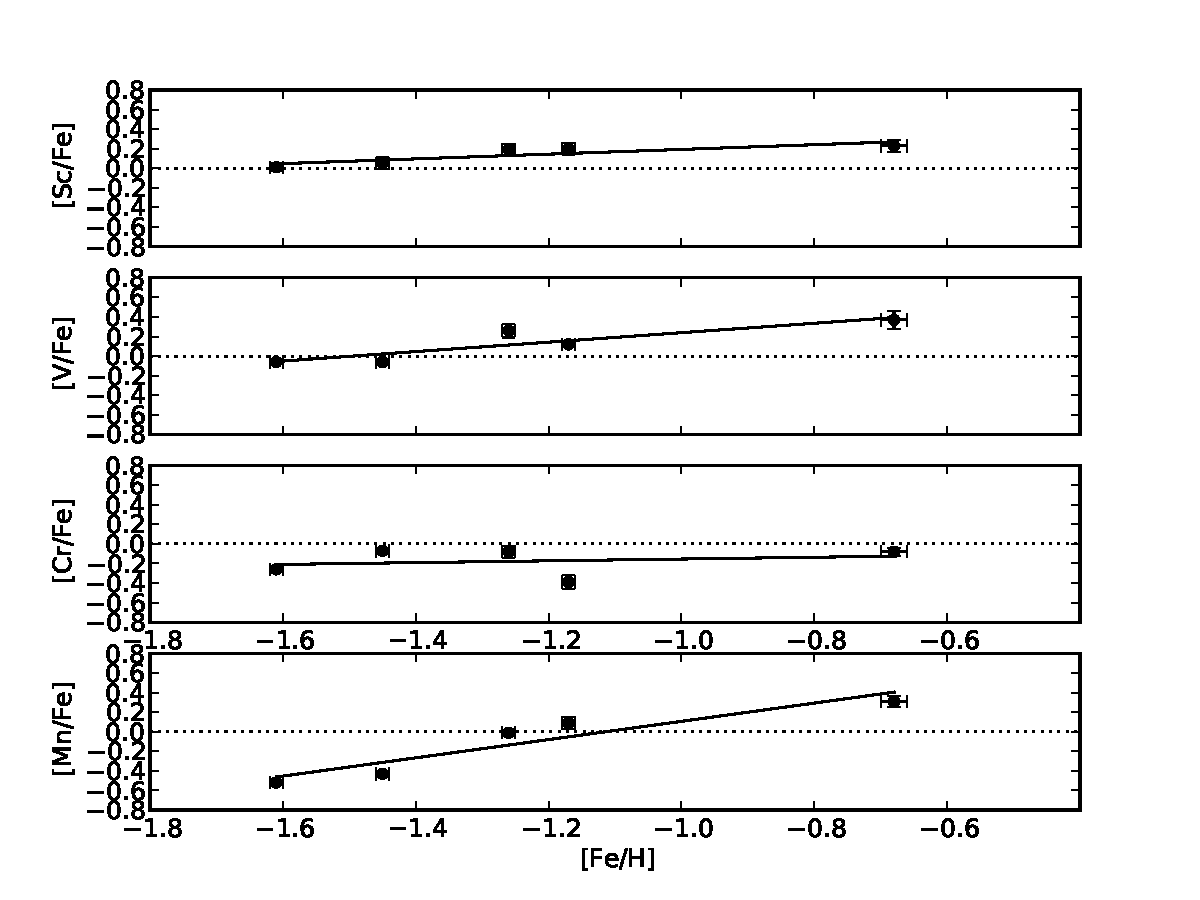
\includegraphics[width=\columnwidth]{./figures/aquarius-fe-peak.pdf}
	\caption{Iron peak element abundances (Sc, V, Cr, Mn, Co and Cu) with respect to iron for all Aquarius stream stars. Ni, an additional Fe-peak element, is discussed in \S\ref{sec:na-ni-relationship} and shown in Figure \ref{fig:na-ni}}
	\label{fig:fe-peak-elements}
\end{figure}



\subsection{Neutron-capture Elements}
Neutron-capture elements (Sr to Eu; ${38 \leqslant Z \leqslant 63}$) can be forged through multiple nucleosynthetic processes. The two primary processes that produce these elements are the rapid ($r$-) process and the slow ($s$-) process. While the $r$-process is theorised to occur in SN explosions, the $s$-process takes place foremost in AGB stars with a significant contribution from massive stars at higher metallicities \citep[e.g.,]{meyer_1994}, although models of rotating massive stars may change this picture \citep{frischknecht;et-al_2012}. 

\subsubsection{Strontium, Yttrium and Zirconium}
\label{sec:weak-s-process-elements}

These light neutron-capture elements generally increase in lock-step with each another. While {[Y\,\textsc{ii}/Fe]} and {[Zr\,\textsc{i}, Zr \textsc{ii}/Fe]} are in good agreement among all candidates, {[Sr\,\textsc{i}/Fe]} ratios are generally lower, with considerable scatter. The {Sr\,\textsc{ii}} lines at 407.7\,nm and 421.5\,nm were not detected in any program or standard stars, although {Sr\,\textsc{i}} was measurable at 664.5\,nm and no obvious telluric contamination was observed. Given that Sr\,\textsc{i} transitions are susceptible to non-LTE effects \citep{hansen;et-al_2013}, we note these Sr abundances should be treated with some caution.

%This is the first study to present first peak $s$-process elemental abundances for five of the six standard stars. Existing data on neutron-capture abundances were not crucial in selecting standard comparison stars: it was more important to cover a range of stellar parameters. 

The Aquarius stream candidates have Y abundances consistent with halo field stars, with the exception of {C222531-145437}. With {[Y/Fe] = 0.79}, {C222531-145437} is significantly over-abundant in Y for its metallicity \citep[see Figure 4 of][]{travaglio;et-al_2004}. {C222531-145437} is consistently over-abundant in Sr and Zr, too. All other program and standard stars have light $s$-process abundances and trends that are consistent with the chemical evolution of the Milky Way.


\subsubsection{Barium and Lanthanum}

Barium is primarily produced through the $s$-process, has appreciable hyperfine and isotopic splitting, and its measurement requires some careful consideration. Solar Ba isotopic ratios from \citet{citation_needed3} have been adopted. Our standard stars have [Ba/Fe] abundances typical of the Milky Way halo. Two standard stars have existing [Ba/Fe] measurements from high-resolution spectra: HD\,44007 and HD\,76932. We find HD\,44007 to have ${\mbox{[Ba/Fe]} = 0.03}$, which is in good agreement with \citet{burris;et-al_2000}, who find {0.05\,dex}. For HD\,76932 our measurement of {$\mbox{[Ba/Fe]} = 0.18$} is in reasonable agreement with the \citet{fulbright_2000} value of $-0.02$\,dex, especially when differences in adopted solar composition are considered.

With one exception, the Aquarius stream candidates have [Ba/Fe] abundance ratios that are indistinguishable from field stars, ranging between ${\mbox{[Ba/Fe]} = -0.10}$ to {0.10\,dex}. The exception is {C222531-085103}, which has an anomalously high barium abundance of ${\mbox{[Ba/Fe]} = 0.62}$. This is $\sim$+0.60\,dex higher than the Milky Way trend at its given metallicity of ${\mbox{[Fe/H]} = -1.26}$. Our two {Ba\,\textsc{ii}} lines in {C222531-085103} are in excellent agreement with each other: [Ba/Fe] = 0.63, and 0.61. 

% [TODO] Lanthanum??




% [TODO] Synthesize Lanthanum
% [TODO] Discuss Lanthanum

\subsubsection{Cerium, Neodymium and Europium}

Europium is primarily produced by the $r$-process, whereas the production of Ce and Nd is split between $s$- and $r$-process. Europium abundances have been determined by synthesising the 664.5\,nm Eu\,\textsc{ii} transition with hyperfine splitting data from \citet{citation_needed5}.

We chose not to use the 643.7\,nm line as it is appreciably blended by a nearby Si\,\textsc{i} line \citep{Lawler;et-al_2001}, and our measurements were consistent with a hidden blend: the 643.7\,nm Eu\,\textsc{ii} abundance was systematically higher than the 664.5\,nm counterpart. One Aquarius stream candidate, {C222531-145437}, appears enhanced in all [$s$-process/Fe] abundance ratios compared to the program and standard sample. However no noteworthy difference in Eu, an $r$-process dominated element, was observed.

% elemental abundances
\begin{figure}[h]
	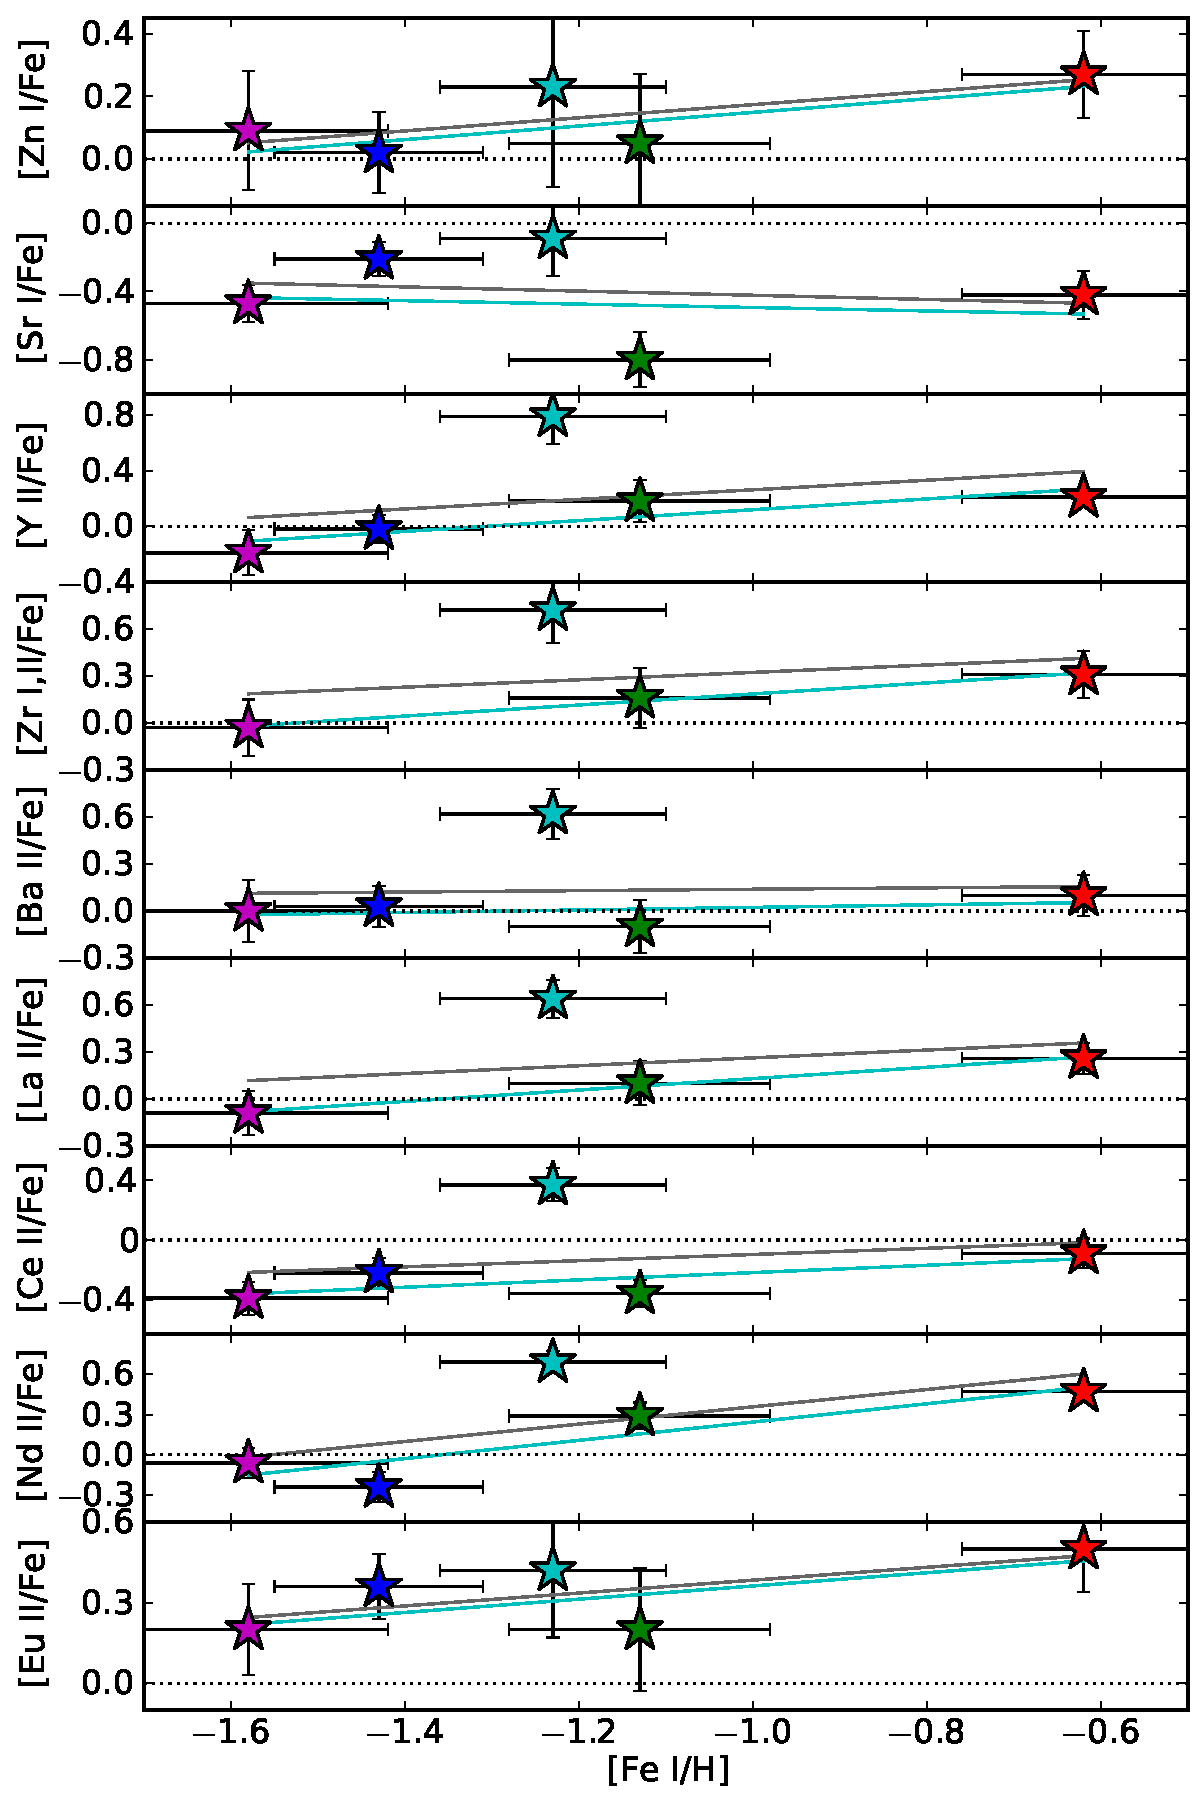
\includegraphics[width=\columnwidth]{./figures/plot-x-on-fe.pdf}
	\caption{Element ratios for Aquarius stream stars. In the case of [Zr/Fe], {[Zr\,\textsc{i}/Fe]} is taken where available and {[Zr\,\textsc{ii}/Fe]} if no measurement was available for {Zr\,\textsc{i}}. See Table \ref{tab:program-star-abundances} for details.}
	\label{fig:x-on-fe}
\end{figure}


\section{Uncertainties}
\label{sec:uncertainties}

\subsection{Uncertainties in Stellar Parameters}
Due to scatter in neutral iron lines measurements, there is a formal uncertainty in our calculated trend line between excitation potential and abundance, as well as between the reduced equivalent width and abundance. We have calculated 1-$\sigma$ uncertainties in effective temperature and microturbulence by independently varying each stellar parameter until the relevant slope matches that formal uncertainty. This process is repeated for positive and negative offsets in temperature and microturbulence to allow for strong asymmetric uncertaintie. The largest absolute offset is taken as the $1\sigma$ uncertainty. For surface gravity, the uncertainty has been calculated by varying $\log{g}$ until the difference in mean Fe\,\textsc{i} - Fe\,\textsc{ii} abundance matches the standard error about the mean for Fe\,\textsc{i} and Fe\,\textsc{ii} in quadrature. The calculated uncertainties are tabulated in Table \ref{tab:stellar-parameter-uncertainties}. 

These uncertainties ignore any correlations between stellar parameters, and therefore are likely to be under-estimated. As such, we have assumed the total uncertainty in stellar parameters to be $\sigma(T_{\rm eff}) = \pm125$\,K, $\sigma(\log{g}) = \pm0.30$\,dex, and $\sigma(v_t) = \pm0.20$ km s$^{-1}$. These adopted uncertainties are higher than any of the measured the uncorrelated uncertainties, and are \textit{extremely conservative}.

\begin{deluxetable}{lccccccccccc}
\tablecolumns{1}
\tabletypesize{\scriptsize}
\tablecaption{Uncorrelated Uncertainties in Stellar Parameters\label{tab:stellar-parameter-uncertainties}}
\tablehead{
    \colhead{Designation} &
	\colhead{$\sigma(T_{\rm eff})$} &
	\colhead{$\sigma(v_t)$} &
	\colhead{$\sigma(\log{g})$} \\
%	\colhead{$\sigma({\rm [M/H]})$} \\
 & (K) & (km s$^{-1}$) & (dex) %& (dex)
 }
\startdata
HD\,41667  	&    53   	&   0.09   &   0.13   \\%&   0.12 \\
HD\,44007 		&    81   	&   0.29   &   0.09   \\%&   0.13 \\
HD\,76932 		&   107  	&   0.08   &   0.19   \\%&   0.10 \\
HD\,136316		&    33   	&   0.15   &   0.12   \\%&   0.11 \\
HD\,141531		&    25   	&   0.05   &   0.13   \\%&   0.06 \\
HD\,142948		&    47   	&   0.10   &   0.11   \\%&   0.10 \\
J221821-183424 	&    42   	&   0.11   &   0.09   \\%&   0.09 \\
C222531-145437  	&    46   	&   0.05   &   0.12   \\%&   0.10 \\
J223504-152834  	&    61   	&   0.08   &   0.05   \\%&   0.12 \\
J223811-104126  	&    49   	&   0.16   &   0.08   \\%&   0.06 \\
C230626-085103  	&    52   	&   0.05   &   0.04   %&   0.12
\enddata
\end{deluxetable}

\subsection{Uncertainties in Chemical Abundances}

The uncertainties in chemical abundances are primarily driven by systematic uncertainties in stellar parameters, with a small contribution of random measurement scatter from individual lines. In order to calculate the abundance uncertainties due to stellar parameters, we have independently varied the stellar parameters by the adopted uncertainties, and measured the resultant change in chemical abundances. For lines requiring synthesis due to hyperfine structure, the difference in chemical abundances has been calculated from EWs. However, the effect of wing broadening due to hyperfine or isotopic splitting was generally small, and we can assume these effects are linear.

The abundance offsets from each variation of stellar parameters has been added in quadrature, along with the standard error about the mean for the line measurements. In some cases, the standard error about the mean is unrealistically small. As discussed earlier in Section \ref{sec:sodium-abundances}, we have conservatively adopted an abundance floor of 0.10\,dex for the standard deviation (i.e. $Max(0.10, \sigma(\log_{\epsilon}X)$). These resultant changes in abundances and total uncertainties are listed for all stars in Table \ref{tab:chemical-abundance-uncertainties}. These total uncertainties have been used in all figures. This provides us with an uncertainty for all abundances, in all stars, of [X/H]. Generally though, we are most interested in the uncertainty in [X/Fe]. In order to calculate this uncertainty, the correlations in uncertainties due to stellar parameters between (X, Fe) need to be considered. We have followed the description in \citet{johnston;et-al_2001} to calculate these correlations, and the overall uncertainties in [X/Fe], which are listed in Table \ref{tab:chemical-abundance-uncertainties} for all program and standard stars.

\begin{deluxetable*}{lcccccc}
\tablecolumns{1}
\tabletypesize{\scriptsize}
\tablecaption{Abundance Uncertainties Due to Stellar Parameters\label{tab:chemical-abundance-uncertainties}}
\tablehead{
 & &  & & & \multicolumn{2}{c}{\textbf{Total Uncertainty}} \\
 \cline{6-7}
	\colhead{Species} &
	\colhead{$T_{\rm eff} +125\,{\rm K}$} &
	\colhead{$\log{g} +0.20\,{\rm dex}$} &
	\colhead{${v_t} +0.30$\,km s$^{-1}$} &
	\colhead{$Max(0.10, \sigma)/\sqrt(N)$} & 
	\colhead{[X/H]} &
	\colhead{[X/Fe]} \\
	 & $\Delta$abundance & $\Delta$abundance & $\Delta$abundance & (dex) & (dex) & (dex)
 }
\startdata
\\
\multicolumn{7}{c}{\textbf{HD 41667}} \\
\hline
O I  		& +0.03		& +0.08		&$-$0.01		& 0.07		& 0.11		& 0.12 \\
Na I  		& +0.13		& +0.00		&$-$0.02		& 0.10		& 0.16		& 0.09 \\
Mg I  		& +0.08		& +0.01		&$-$0.01		& 0.05		& 0.10		& 0.10 \\
Al I  		& +0.10		& +0.01		&$-$0.01		& 0.06		& 0.11		& 0.07 \\
Si I  		& +0.02		& +0.03		&$-$0.02		& 0.04		& 0.06		& 0.13 \\
K I  		& +0.14		&$-$0.03		&$-$0.17		& 0.10		& 0.24		& 0.15 \\
Ca I  		& +0.13		&$-$0.01		&$-$0.10		& 0.05		& 0.17		& 0.05 \\
Sc II  	&$-$0.03		& +0.08		&$-$0.08		& 0.05		& 0.13		& 0.17 \\
Ti I  		& +0.22		& +0.01		&$-$0.01		& 0.05		& 0.22		& 0.04 \\
Ti II 		&$-$0.04		& +0.07		&$-$0.15		& 0.14		& 0.23		& 0.25 \\
V I 		& +0.25		& +0.01		&$-$0.03		& 0.05		& 0.26		& 0.09 \\
Cr I 		& +0.23		& +0.00		&$-$0.20		& 0.03		& 0.31		& 0.14 \\
Cr II  	&$-$0.07		& +0.08		&$-$0.06		& 0.07		& 0.14		& 0.22 \\
Mn I  		& +0.17		& +0.01		&$-$0.07		& 0.06		& 0.19		& 0.05 \\
Fe I  		& +0.16		& +0.01		&$-$0.07		& 0.02		& 0.17		& \nodata \\
Fe II  	&$-$0.10		& +0.08		&$-$0.04		& 0.03		& 0.14		& \nodata \\
Co I  		& +0.18		& +0.03		&$-$0.01		& 0.04		& 0.19		& 0.04 \\
Ni I  		& +0.12		& +0.03		&$-$0.01		& 0.05		& 0.13		& 0.03 \\
Cu I  		& +0.19		& +0.03		&$-$0.16		& 0.10		& 0.27		& 0.10 \\
Zn I  		&$-$0.03		& +0.06		&$-$0.09		& 0.07		& 0.14		& 0.19 \\
Sr I  		& +0.24		& +0.01		&$-$0.06		& 0.10		& 0.27		& 0.11 \\
Y II  		& +0.00		& +0.08		&$-$0.09		& 0.09		& 0.15		& 0.15 \\
Zr I  		& +0.27		& +0.01		& +0.00		& 0.07		& 0.28		& 0.13 \\
Zr II  	& +0.00		& +0.08		&$-$0.01		& 0.10		& 0.13		& 0.17 \\
Ba II 		& +0.01		& +0.06		&$-$0.21		& 0.07		& 0.23		& 0.19 \\
La II 		& +0.01		& +0.07		&$-$0.02		& 0.07		& 0.10		& 0.14 \\
Ce II 		& +0.04		& +0.08		&$-$0.04		& 0.09		& 0.13		& 0.11 \\
Nd II 		& +0.02		& +0.06		&$-$0.07		& 0.03		& 0.10		& 0.11 \\
Eu II 		&$-$0.05		& +0.04		&$-$0.06		& 0.10		& 0.13		& 0.22
\enddata
\tablenotetext{}{Table \ref{tab:chemical-abundance-uncertainties} is published for all standard and program stars in the electronic edition. A portion is shown here for guidance regarding its form and content.}
\end{deluxetable*}


\section{Discussion}
\label{sec:discussion}
% wylie de boer discrepancies


\subsection{Stellar Parameter Discrepancies with \\ \citet{wylie-de-boer;et-al_2012}}

We seek to investigate the nature of the Aquarius stream. Specifically, the globular cluster origin suggested by \citet{wylie-de-boer;et-al_2012}. For the four stars common to both samples, the stellar parameters reported in \citet{wylie-de-boer;et-al_2012} differ to our values listed in Table \ref{tab:stellar-parameters}. \citet{wylie-de-boer;et-al_2012} deduce their stellar parameters by minimizing the $\chi^2$ difference between the observed spectra and synthetic spectra from the \citet{munari;et-al_2005} spectral library. In general, effective temperatures between the two studies agree within the uncertainties. The only aberration is {J223811-104126}, where we find an effective temperature of {5190\,K}, $\sim$450\,K cooler than the {5646\,K} found by \citet{wylie-de-boer;et-al_2012}. Similarly, \citet{williams;et-al_2011} report a hotter effective temperature of {5502\,K} from low-resolution spectra. This is the largest discrepancy we see in any of our standard or program stars.

Photometric temperature relationships support our spectroscopic temperature for J223811-104126. The \citet{ramirez;melendez_2005} relationship for giants suggests an effective temperature of 5240\,K, which is 50\,K warmer than our spectroscopically-derived temperature. Furthermore, the metallicity-independent $J-K$ colour-$T_{\rm eff}$ relationship for giants by \citet{alonso;et-al_1999} yields an effective temperature of 5215\,K, 25\,K warmer than our spectroscopic temperature. As a test, we set the temperature for {J223811-104126} to be 5600\,K -- within the temperature regime reported by \citet{williams;et-al_2011} and \citet{wylie-de-boer;et-al_2012}. The slopes and offsets in abundance with excitation potential and REW were large: ${m_{\rm Fe\,\textsc{i}} = -0.099}$\,dex\,eV$^{-1}$, 0.162\,dex, ${m_{\rm Fe\,\textsc{ii}} = -0.133}$\,dex\,eV$^{-1}$, $-0.033$\,dex respectively, and in doing so we could not find a representative solution for this temperature. 

\citet{williams;et-al_2011} and \citet{wylie-de-boer;et-al_2012} find {J223811-104126} to be a sub-giant/dwarf, with a surface gravity {$\log{g} = 4.16$} and {4.60} respectively. We note that the \citet{williams;et-al_2011} and \citet{wylie-de-boer;et-al_2012} effective temperatures for J223811-104126 are 150-300\,K hotter than the \citet{casagrande;et-al_2010} $J-K$ photometric temperature calibration for dwarfs and sub-giants. We find the surface gravity for {J223811-104126} to be {$\log{g} = 2.93 \pm 0.30$\,dex}, placing this star at the base of the red giant branch.

With the exception of {J223811-104126}, our surface gravities are largely in agreement with \citet{wylie-de-boer;et-al_2012}. The only other noteworthy difference is for {J221821-183424}, where we find a lower gravity of {$\log{g} = 0.88 \pm 0.30$} and \citet{wylie-de-boer;et-al_2012} find {$\log{g} = 1.45 \pm 0.35$\,dex}. Given the difference in the $S/N$  between these studies, this difference is not too concerning. \citet{wylie-de-boer;et-al_2012} calculate the microturbulence from empirical relationships derived by \citet{reddy;et-al_2003} for dwarfs and \citet{fulbright_2000} for giants. These relationships are based on the effective temperature and surface gravity. Our published microturbulent velocities agree excellently with the values presented in \citet{wylie-de-boer;et-al_2012}, again with the exception of {J223811-104126}, where the difference in $v_{t}$ is directly attributable to the offsets in other observables.

Of all the stellar parameters, metallicities exhibit the largest discrepancy between the two studies. In the \citet{wylie-de-boer;et-al_2012} study, after the stellar parameters ($T_{\rm eff}$, $\log{g}$, $v_{t}$, and an initial [M/H] estimate) were determined through a $\chi^2$ minimisation, the authors synthesised individual {Fe\,\textsc{i}} and Fe\,\textsc{ii} lines using \textsc{moog}. \citet{castelli;kurucz_2003} stellar atmosphere models were employed (K. Freeman, private communication, 2013) -- the same ones used in this study -- albeit the interpolation schemes will have subtle differences. The median abundance of synthesised {Fe\,\textsc{i}} lines was adopted as the overall stellar metallicity, and scaled relative to the Sun using the \citet{grevesse;sauval_1998} Solar composition.

The study of \citet{wylie-de-boer;et-al_2012} is of slightly lower resolution ($\mathcal{R} = 25,000$ compared to $\mathcal{R} = 28,000$ presented here), but with a much lower $S/N$ ratio: ${\sim{}25\,{\rm pixel}^{-1}}$ compared to {$>$100\,pixel$^{-1}$} achieved here. The line list employed in the \citet{wylie-de-boer;et-al_2012} utilised astrophysical oscillator derived from a reverse solar analysis on the Solar spectrum. However, there are very few transitions listed in their line list: a maximum of 14 {Fe\,\textsc{i}} lines and 3 {Fe\,\textsc{ii}} lines were available. For contrast, our analysis is based on 63 {Fe\,\textsc{i}} and 13 {Fe\,\textsc{ii}} clean, unblended lines. 

% Removed at David Yong's behest
%Given the metallicity of these candidates and the reasonable wavelength coverage (4120-6920\,{\AA}) of the \citet{wylie-de-boer;et-al_2012} data, it is somewhat surprising that there were not more transitions available for analysis. 

Suspecting the differing line lists may contribute to the metallicity discrepancy, we re-analysed our data using the \citet{wylie-de-boer;et-al_2012} line list and stellar parameters. Indeed, in doing so we arrive at reasonably similar metallicities to \citet{wylie-de-boer;et-al_2012}. Without using their published stellar parameters a priori, in a ``blind'' analysis employing just the \citet{wylie-de-boer;et-al_2012} line list, we find stellar parameters similar to \citet{wylie-de-boer;et-al_2012}. However, given the small numbers of lines used, even subtle changes to the stellar parameters can produce large variations to both the individual and mean Fe abundances. Additionally, we note that one {Fe\,\textsc{i}} transition at 642\,nm in the \citet{wylie-de-boer;et-al_2012} line list was either not detected at the {3$\sigma$} level -- even though the $S/N$ at this point exceeds {115\,pixel$^{-1}$} in every observation -- or it was blended with a stronger neighbouring transition.

Given the overall data quality and the lack of suitable Fe lines available for analysis, it appears the Aquarius stream stars conspired to present a tight metallicity distribution of {$\sigma(\mbox{[Fe/H]}) = 0.10$\,dex}. When viewed in light of enhanced [Ni/Fe] and [Na/Fe] abundance ratios, \citet{wylie-de-boer;et-al_2012} interpreted this chemistry as a signature of a globular cluster origin for the Aquarius stream. 

\subsection{The Aquarius Stream Metallicity Distribution}

%This is largely because they are primarily -- and somewhat incorrectly -- considered to be a single stellar populations, originating from a lone, largely homogenous proto-stellar cloud. Observations have demonstrated that this is not always the case: many globular clusters clearly host multiple stellar populations. The separation between these sub-populations is identifiable through chemical abundances, and often from photometry alone. 

This study of high-resolution spectra with high $S/N$ reveals a much broader metallicity distribution for the stream. With just 5 stars we find the metallicity varies from {$\mbox{[Fe/H]} = -0.63$} to {$-1.58$\,dex}. Although this is a small sample, we find the mean abundance and standard deviation to be {$\mbox{[Fe/H]} = -1.20 \pm 0.33$}. 

If the metallicity dispersion were smaller, as found by \citet{wylie-de-boer;et-al_2012}, a globular cluster scenario may be plausible. Classical globular clusters typically exhibit very little dispersion in metallicity. An intrinsic [Fe/H] dispersion of 0.33\,dex -- ignoring error contribution -- is substantially larger than that seen in any globular cluster, with the exception of the unusual system $\omega$-Centauri. In that cluster the total abundance range is about $\Delta$[Fe/H] $\sim$ 1.4\,dex: from $-$2 to $-$0.6 \citep[e.g.][]{marino;et-al_2011}, and many sub-populations have been identified \citep[e.g.,][]{johnson_pilachowski_2010}. 

Other clusters with established intrinsic [Fe/H] dispersions include M54 -- a nuclear star cluster of the Sagittarius dSph -- where $\sigma_{\rm int}$([Fe/H])$ = 0.19$ \citep{carretta;et-al_2010}, and M22, where the interquartile range in [Fe/H] is $\sim{}$0.24 dex \citep{da_costa;et-al_2009,marino;et-al_2009,marino;et-al_2011}. There are a few clusters where the intrinsic dispersion is $\sim$0.10, namely NGC 1851 \citep{carretta;et-al_2011}, NGC 5824 \citep{saviane;et-al_2012}, and NGC 3201 \citep{simmerer;et-al_2013}. These globular clusters are outliers, and even in these unusual systems, only one or two system could plausibly match the abundance spread observed in the Aquarius stream \citep[e.g. see Figure 4 in][]{simmerer;et-al_2013}. In fact, the Aquarius stream metallicity distribution -- on its own -- is large enough to be reconcilable with dSph galaxies like Fornax or Sagittarius, however the $\log(L)-$[Fe/H] relationship would suggest an extremely luminous system on the order of $L_{\rm tot} \sim 10^{7.5}L_\odot$ \citep{kirby;et-al_2011}.  However, the Aquarius stream stars exhibit [Ba/Y] (e.g. heavy/light $s$-process) abundance ratios between $-$0.24 and +0.19, significantly lower than the [Ba/Y] $\geq$ 0.5 level generally observed in the present day dSphs \citep{venn;et-al_2004}.

\subsection{The Na-O Relationship}

% From DY:
%>Just a personal preference, I think you can substantially shorten the text from "Between generations of stars within a globular cluster �" to the end of the subsection. 

%>The pertinent points to make are the fact that O depletion and Na synthesis require temperatures that cannot be readily attained in 0.8M_sun giants, i.e., those currently on the RGB. Additionally, the temperatures required for O-Na synthesis are *not* attained in main sequence stars, nor is there any plausible mixing mechanism to transport processed material to the atmosphere. Thus, the O-Na anticorrelation cannot be due to internal nucleosynthesis and thus an external source/mechanism is demanded. 

%>You have already noted the ubiquitous GC O-Na anticorrelation, and can then jump to the final two para's of this subsection. 

Extensive studies of stars in globular clusters have revealed variations in light element abundances, most notably an anti-correlation in sodium and oxygen content \citep[see][and references therein]{norris;da_costa_1995,carretta;et-al_2009a}. This chemical pattern has been identified in every well-studied globular cluster, although the magnitude and shape of the anti-correlation varies from cluster to cluster.


%Between generations of stars within a globular cluster, oxygen is converted into nitrogen, thereby reducing the overall oxygen abundance. Even though oxygen undergoes internal mixing during its evolution along the giant branch, the detection of this chemical pattern in unevolved stars led to the conclusion that observed abundance variations due to mixing are limited to lithium, carbon and nitrogen. Therefore, the light element anti-correlation requires a different astrophysical explanation.

Sodium is primarily produced through carbon burning in massive stars by the dominant $^{12}\mbox{C}(^{12}\mbox{C}, p)^{23}\mbox{Na}$ reaction. The final Na abundance is dependent on the neutron excess of the star, which slowly increases during carbon burning due to weak interactions \citep{arnett;truran_1969}. Massive stars ($>10 M_\odot$) eventually deliver their synthesized sodium to the interstellar-medium through {SN\,\textsc{ii}} explosions. Because the eventual {SN\,\textsc{ii}} explosion is devoid of any significant $\beta$-decay processes, the neutron excess of the ejected material is representative of the pre-explosive abundance. The ejected material eventually condenses to form the next generation of stars, which will have a net increase in their neutron excess with respect to their predecessors. Since the sodium production rate is correlated with the neutron excess, an overall increase in the total sodium content \textit{and} Na-production rate between stellar generations can be expected. The sodium content also becomes important for production of nickel during the {SN\,\textsc{ii}} event (see Section \ref{sec:na-ni-relationship}) because $^{23}$Na is the only stable isotope produced in significant quantities during the C- or O-burning stages. 

Oxygen depletion is likely the result of complete CNO burning within the stellar interior. The nucleosynthetic pathways that produce the {Na-O} anti-correlation are well understood to be proton-capture nucleosynthesis at high temperatures \citep{prantzos;et-al_2007}. However, the temperatures required to produce these patterns are not expected within the interiors of globular cluster stars. While the exact mechanism for which these conditions occur remains under investigation, we can describe the abundance variation as an external oxygen depletion (or dilution) model with time. Through comparisons with existing globular clusters, we can make inferences on the star-formation history of a system by measuring sodium and oxygen abundances in a sample of its stars. 

\begin{figure*}[t!]
	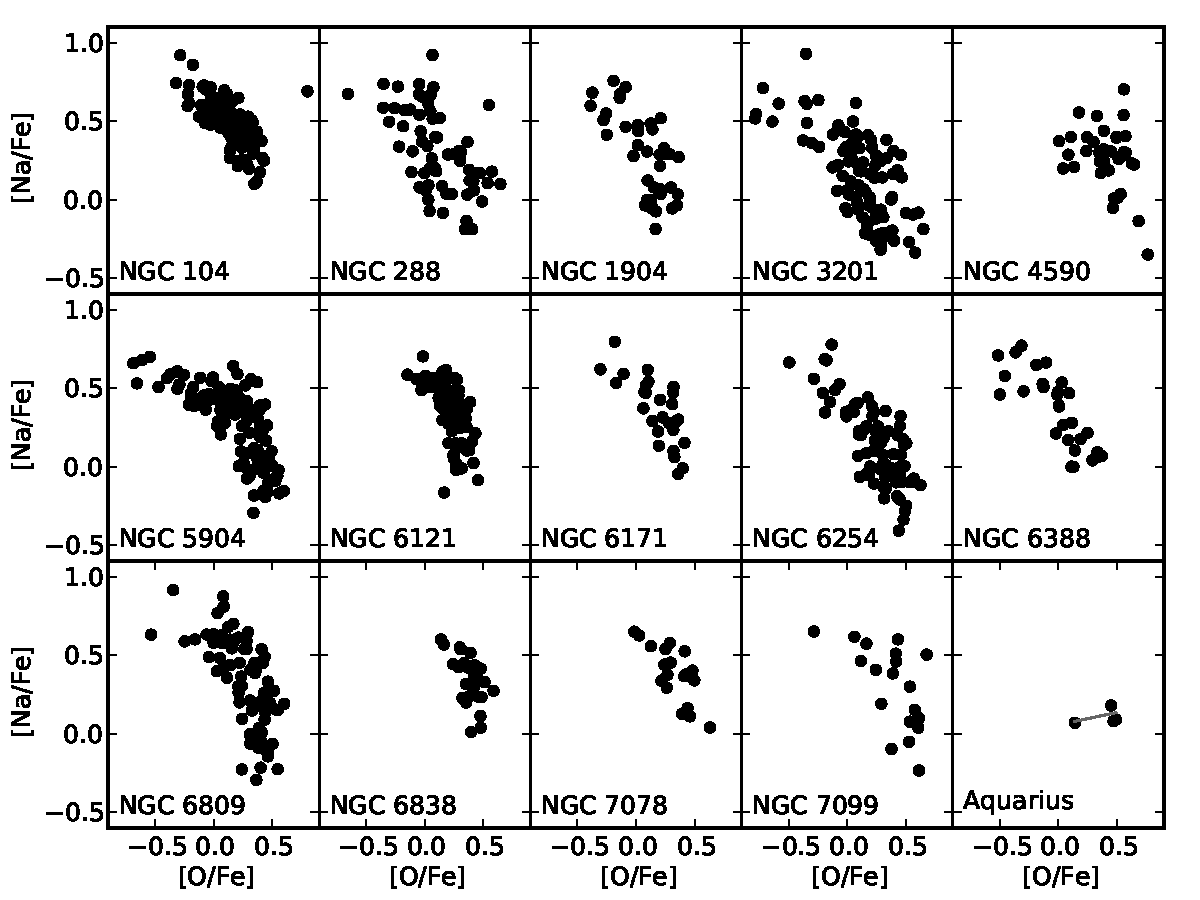
\includegraphics[width=\textwidth]{./figures/aquarius-o-na-cluster.pdf}
	\caption{Oxygen and sodium abundances for 14 classical globular clusters from \citet{carretta;et-al_2009a}, demonstrating the clear inverse {Na-O} correlation, ubiquitous to all well-studied globular clusters. The [O/Fe] and [Na/Fe] abundances from this study for the 5 Aquarius stream stars (1/3 of the entire stream) are also shown in the last panel.}
	\label{fig:o-na-clusters}
\end{figure*}


 %Thus, an increase in the sodium abundance between generations of massive stars is a natural consequence of nucleosynthesis. 
 
 
 
 %A small fraction of $^{22}$Na is also forged through proton-capture on $^{21}$Ne in the carbon shell, an effect which is enhanced by neutrinos spallating abundant elements like $^{16}$O and $^{20}$Ne, making free protons available for capture \citep{woosley;weaver_1995}.



%\citet{carretta;et-al_2009a} defined three components of stars exhibiting an inverse {Na-O} correlation within a population: primordial, intermediate, and extreme components. The [Na/Fe] and [O/Fe] abundances for a given star define which component it belongs to. An intermediate component -- the second-generation of stars -- will have super-solar sodium abundances and demonstrate a slight depletion in oxygen content. Stars with {[O/Na]$ > -0.9$} are classified as belonging to the extreme component, a signature indicating long-lasting star-formation.


%Primordial (first-generation) stars are those with sodium and oxygen abundances which are similar to field stars of the same metallicity. An intermediate component -- the second-generation of stars -- will have super-solar sodium abundances and demonstrate a slight depletion in oxygen content. The oxygen exhaustion rate is ultimately dependent on the star-formation history of the cluster environment.  The extreme O-depletion component has only been observed in a few clusters (preferentially more massive clusters with extended horizontal branches), indicating a long-lasting star-formation history in more massive clusters.

%Careful consideration must be given when inferring star-formation histories from observed stellar abundances.
Such inferences must be made with careful consideration. In addition to the normal care afforded for measuring elemental abundances from high-resolution spectroscopic data, attention must be given to telluric absorption, contamination from Ni\,\textsc{i}, as well as non-LTE and 3D effects when determining oxygen abundances. Furthermore, when characterising the oxygen depletion rate -- the strength of the {Na-O} anti-correlation in a globular cluster -- it is vital to sample, where possible, stars belonging to all three components \citep[primordial, intermediate and extreme, see][]{carretta;et-al_2009a}. If only a primordial sample of stars is observed, their [Na/Fe] and [O/Fe] abundances will be, by definition, indistinguishable from field stars of a similar metallicity. In such a scenario any inferred anti-correlation could equally be explained by small abundance variations or observational uncertainties. 

%Finally, one must exclude the possibility that a {Na-O} anti-correlation is being inferred from a composite sample of field stars with a fractional contribution of stars that were born in globular clusters. \citet{ramirez;et-al_2012} estimate at least 3\%$\pm$2\% of the local field stars in this metallicity regime were born in globular clusters.


% [O/Fe], [Na/Fe]
\begin{figure}[t!]
	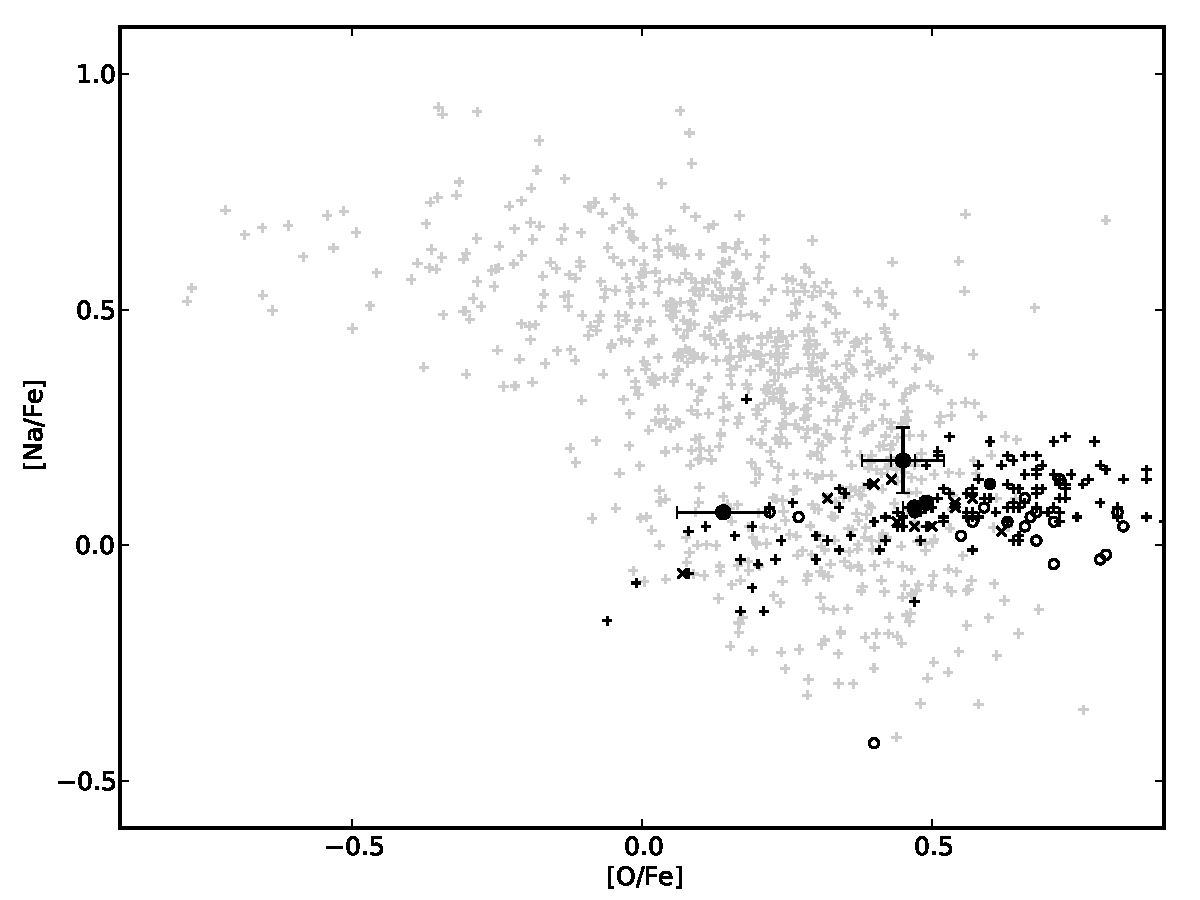
\includegraphics[width=\columnwidth]{./figures/aquarius-o-na-halo.pdf}
	\caption{Oxygen and sodium abundances for thick disc ($+$), thin disc ($\times$) and halo ($\circ$) stars from \citet{reddy;et-al_2006}, and globular cluster stars from \citet{carretta;et-al_2009a} (grey symbols). The Aquarius stream stars are also shown (\textbullet), illustrating how their [O/Fe], [Na/Fe] content is not dissimilar from Galactic stars. Ambiguous thick disc/thin disc stars in \citet{reddy;et-al_2006} are marked with thick disc symbols ($+$), as are uncertain thick disc/halo stars with halo symbols ($\circ$).}
	\label{fig:o-na}
\end{figure}

\citet{wylie-de-boer;et-al_2012} measured sodium and oxygen abundances for four of their six Aquarius stream members. These measurements exist for only three stars common to both samples, as the data quality for {J223811-104126} in the \citet{wylie-de-boer;et-al_2012} was too low to permit oxygen measurements. We have measured sodium and oxygen abundances for all of our stars, which are plotted in Figures \ref{fig:o-na-clusters} and \ref{fig:o-na}. These figures employ the corrected [O/Fe] value for {J223811-104126} rather than a conservative upper limit (see Section \ref{sec:oxygen-abundances}).


% how do our values compare with Wylie de boer

% star 		| mine 				| hers
% C222531	| 0.10 +/- 0.01 (2)	| 0.00 +/- 0.15
% C2306265	| 0.21 +/- 0.00 (2)| ...
% J221821	| 0.09 +/- 0.10 (1)| 0.03 +/- 0.15
% J223504	| 0.26 +/- 0.07 (3)| 0.28 +/- 0.21
% J223811	| 0.08 +/- 0.00 (1)| 0.04 +/- 0.15


The \citet{wylie-de-boer;et-al_2012} measurements show two stars with solar levels of [Na/Fe] -- identical to field star abundances for their metallicity -- and two stars with enhanced sodium content: {J223504-152834} and {J232619-080808}. We also find {J223504-152834} to be sodium-enhanced, whereas the second star in their study, {J232619-080808}, is not in our sample. We find the additional star not present in the \citet{wylie-de-boer;et-al_2012} sample, {C2306265-085103}, to be sodium-enhanced to almost the same level of {J223504-152834} with {$\mbox{[Na/Fe]} = 0.26$}. The sodium-enhanced stars exhibit no depletion of oxygen; their chemistry does not demonstrate a {Na-O} anti-correlation. 

%In fact, they have a slight positive relationship: the sodium-enhanced stars in the \citet{wylie-de-boer;et-al_2012} study show an increased oxygen content (within the uncertainties), contrary to an expected oxygen depletion between stellar generations within a globular cluster. With our revised oxygen abundances and two sodium-enhanced stars, we find a very slight positive relationship of X.XX +/- X.XX. Thus, there continues to be {\it no evidence of a Na-O anti-correlation in the Aquarius stream}. 

If the Aquarius stream is the result of a disrupted globular cluster, a large part of the picture must still be missing. Almost all of the Aquarius stream stars studied to date (either in this sample or the \citet{wylie-de-boer;et-al_2012} study), would be unambiguously classified as belonging to a ``primordial'' component, with chemistry indistinguishable from field stars. Identifying more Aquarius stream members belonging to the intermediate component with strong oxygen depletion, or perhaps members of an extreme component, would be convincing evidence for a {Na-O} anti-correlation and a globular cluster origin. Three stream stars identified to date (including two from this sample) might tenuously be classified as members of an intermediate population, with only a slight enhancement in sodium and no oxygen-depletion. Recall our [Na/Fe] abundance ratios appear systematically higher in our standard stars when compared to the literature. Thus, if the strength of any {Na-O} relationship is to be used to vet potential disrupted hosts for the Aquarius stream, many more stream members will need to be identified and observed spectroscopically with high-resolution and high $S/N$. In the absence of such data, no evidence exists for a {Na-O} anti-correlation in the Aquarius stream.

\subsection{The Al-Mg Relationship}

%The Na-O anti-correlation is likely the result of complete CNO and Ne-Na cycles of proton reactions in globular cluster stars. There is also evidence in some clusters that the Mg-Al nucleosynthesis cycle is also active. 

%An inverse relationship between sodium and oxygen is not the only chemical pattern commonly observed in globular clusters.
Although not ubiquitous to every system, many clusters exhibit an anti-correlation between aluminium and magnesium. This is perhaps unsurprising, given the nucleosynthetic pathways for these elements. In addition to the CNO cycle operating during hydrogen burning, the {Mg-Al} chain can also operate under extreme temperatures \citep[$T \sim 8 \times 10^{6}\,$K;][]{arnould;et-al_1999}. In these conditions, aluminium is produced by proton-capture of magnesium, beginning with $^{24}$Mg to $^{25}$Al. The relative lifetime of $\beta$-decay to proton-capture allows for the production of unstable $^{27}$Si through proton-capture. Seconds later, the isotope decays to $^{27}$Al, completing the $^{27}$Si path of the Mg-Al chain. The alternative process onwards from $^{26}$Al involves proton-capture to $^{26}$Mg, but this process requires even higher temperatures ($T \sim 7 \times 10^{6}\,$K).

The Mg-Al cycle can explain the observed anti-correlation observed in some globular clusters, and some AGB models can predict such a pattern (e.g., \citet{ventura;et-al_2011} but see nucleosynthesis yields from \citet{karakas;lattanzio_2007} and \citet{karakas_2010}). Thus, while the pathways for creating these chemical patterns are understood, the temperatures required to produce this chain are much higher than expected for stellar interiors, so the exact site and requisite conditions are lacking a full description.

\citet{wylie-de-boer;et-al_2012} published magnesium and aluminium abundances for five stars in their Aquarius sample. No inverse correlation is present in their data; their abundances are indistinguishable from field stars. The [(Mg, Al)/Fe] abundance ratios tabulated in Table \ref{tab:program-star-abundances} are generally in agreement with the \citet{wylie-de-boer;et-al_2012} sample, and we also find no {Mg-Al} anti-correlation. Given that we do not find a {Na-O} anti-correlation, it is not surprising that a {Mg-Al} anti-correlation is also not observed. 

%Two candidates are in good agreement: {J221821-183424} and {J223811-104126}, albeit the data quality in the \citet{wylie-de-boer;et-al_2012} study did not permit the measurement of aluminium for {J223811-104126}. The other two stars common between studies are {C222531-145437} and {J223504-152834}, which we found to be the most abundant in both magnesium and aluminium. 





% how do our values compare with Wylie de boer
%							[Mg/Fe]						[Al/Fe]					| [Mg?]	| [Al?]
% star 		| mine 				| hers			| mine			| hers			| 
% C222531	| 0.53 +/- 0.06		| 0.32 +/- 0.05	| 0.71 +/- 0.04	| 0.38 +/- 0.12	| No, + | No, +
% C2306265	| 0.44 +/- 0.05		| ...			| 0.33 +/- 0.04	| ...			| N/A	| N/A 
% J221821	| 0.35 +/- 0.05		| 0.30 +/- 0.01	| 0.21 +/- 0.10	| 0.29 +/- 0.12	| Yes +	| Yes -
% J223504	| 0.51 +/- 0.09		| 0.33 +/- 0.05	| 0.29 +/- 0.05	| 0.21 +/- 0.03	| No +	| No +
% J223811	| 0.34 +/- 0.01		| 0.30 +/- 0.06	| 0.11 +/- 0.10	| ...			| Yes +	| N/A



% Mg-Al
\begin{figure}[h!]
	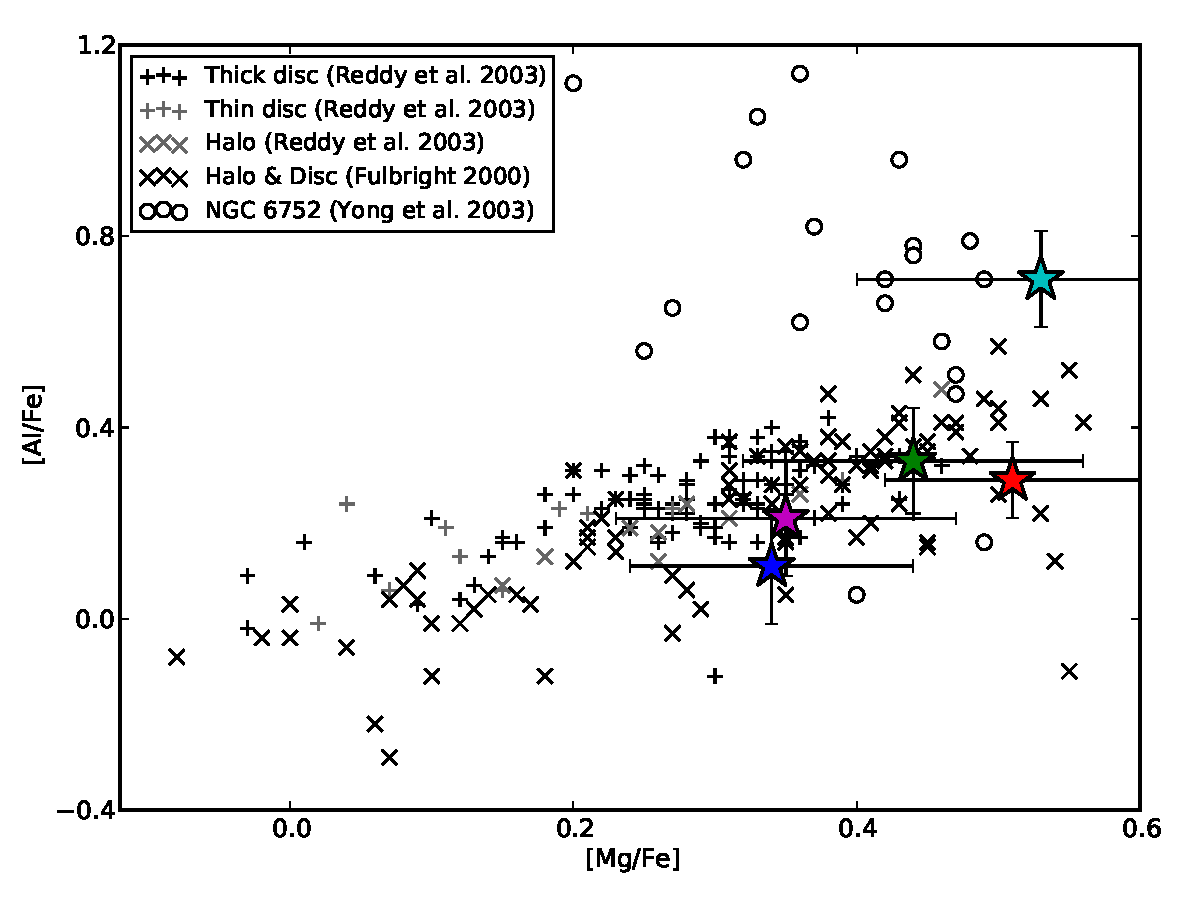
\includegraphics[width=\columnwidth]{./figures/aquarius-mg-al.pdf}
	\caption{Magnesium and aluminium abundances for Aquarius stream stars (\textbullet), and Milky Way halo/disc stars from \citet{reddy;et-al_2003} ($+$) and \citet{fulbright_2000} ($\circ$). The chemically peculiar star, {C222531-145437}, is marked.}
	\label{fig:mg-al}
\end{figure}



%The [Mg/Fe] and [Al/Fe] abundances found for the five Aquarius stream stars in this sample are illustrated in Figure \ref{fig:mg-al}.
However it {\it is} surprising that we find such a strong positive relationship in [Mg/Fe] and [Al/Fe], with a best-fitting slope of ${{\rm [Al/Fe]} = 2.08\times\mbox{[Mg/Fe]} - 0.57}$. If we exclude the chemically peculiar star {C222531-145437}, the slope decreases to {${\rm [Al/Fe]} = 0.96\times\mbox{[Mg/Fe]} - 0.16$}, a near 1:1 relationship. Even when a {Mg-Al} anti-correlation is not detected in globular clusters, there is generally more scatter in [Al/Fe] at near-constant [Mg/Fe] \citep[e.g. see Figure \ref{fig:mg-al} or ][]{carretta;et-al_2009a}. This is because Mg is much more abundant than Al, requiring only a small amount of Mg atoms to be synthesized to Al before the differences in $\log\epsilon{}$Al become appreciable, whilst the observed Mg abundance could remain within the uncertainties.


% Mg-Al
%\begin{figure*}[t!]
%	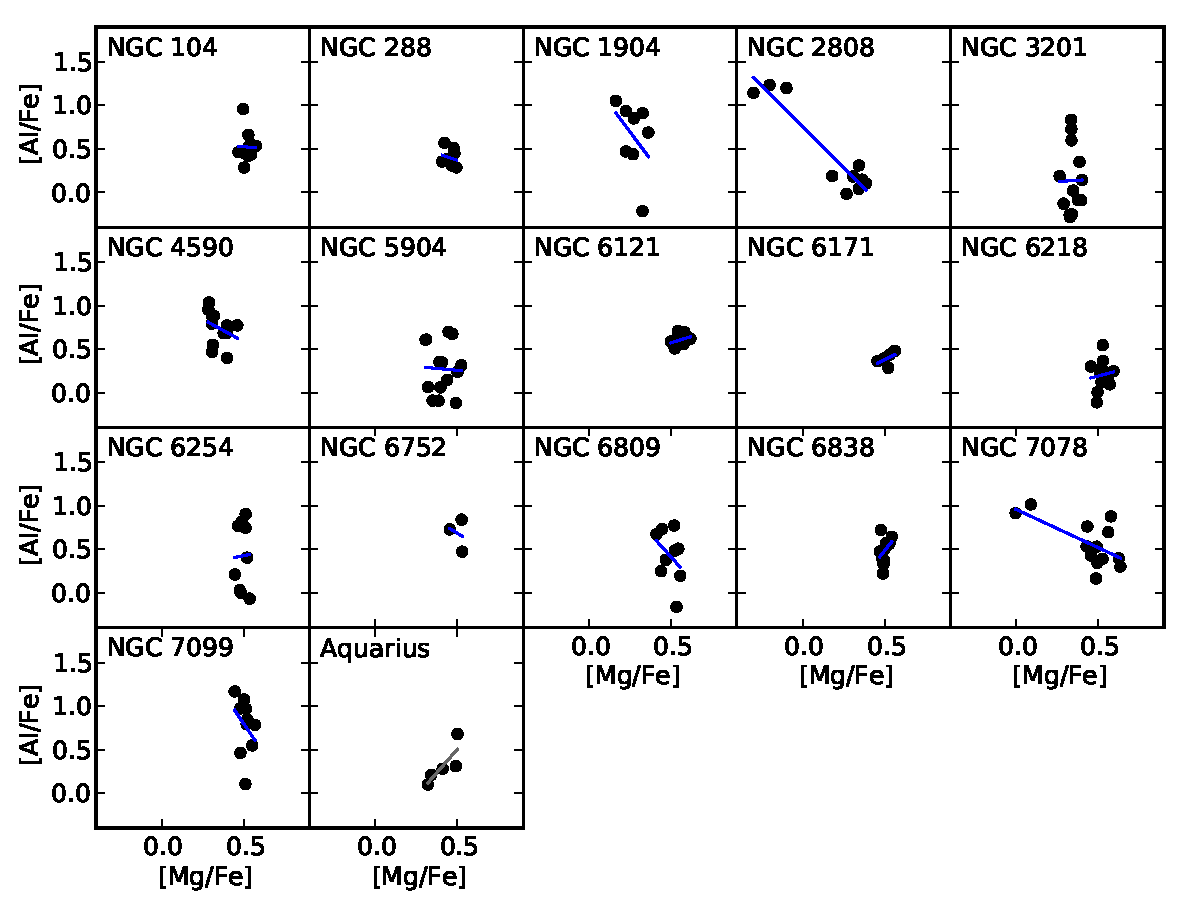
\includegraphics[width=\textwidth]{./figures/aquarius-mg-al-cluster.pdf}
%	\caption{[Mg/Fe] and [Al/Fe] abundances for stars in 16 globular clusters from \citet{carretta;et-al_2009a} and for the five Aquarius stream stars. The inverse {Mg-Al} correlation is illustrated, most obviously in {NGC 2808} and {NGC 1904}. The strong positive correlation observed in Aquarius is in stark contrast with other classical globular clusters.}
%	\label{fig:mg-al}
%\end{figure*}

No classical globular clusters exhibit a positive correlation, and nor is such a pattern expected in globular clusters. However, a positive relationship between magnesium and aluminium can result from {SN\,\textsc{ii}} contributions to the local interstellar medium. Intermediate-mass ($\gtrsim$4$M_\odot$) AGB models can also contribute towards a positive correlation between aluminium and magnesium. Under extreme temperatures ($T \gtrsim 300 \times 10^{6}\,$K), substantial $^{25}$Mg and $^{26}$Mg are produced by $\alpha$-capture onto $^{22}$Ne by the $^{22}$Ne($\alpha$,n)$^{25}$Mg and $^{22}$Ne($\alpha$,$\gamma$)$^{26}$Mg reactions respectively \citep[e.g.,][]{karakas;et-al_2006}. Depending on uncertain numerical details of the stellar model, the third dredge-up can mix significant quantities of $^{25}$Mg and $^{26}$Mg into the photosphere, even more than the quantity of $^{26}$Al produced through the {Mg-Al} cycle. Therefore, a positive relationship between magnesium and aluminium can occur if there has been significant contributions from intermediate-mass AGB stars \citep[][but see results in \citet{ventura;et-al_2011}]{karakas;lattanzio_2003}.
 
An unrealistically high fraction of intermediate-mass AGB stars would be required to produce the same chemical signature of a single {SN\,\textsc{ii}} event. Given the efficiency of chemical mixing following supernovae, the observed positive {Mg-Al} correlation in the thick disc is likely the result of {SN\,\textsc{ii}} events. Distinguishing between these processes observationally requires careful measurements of magnesium isotope abundances $^{24}$Mg (indicating supernovae mixing), $^{25}$Mg and $^{26}$Mg (suggesting significant AGB contribution), which is not possible given our $S/N$ or spectral resolution. In either scenario, we can summarise that the strong Mg-Al relationship provides additional chemical evidence against a globular cluster scenario for the Aquarius stream, and the chemistry is suggestive of Milky Way disc stars.

\subsection{The Na-Ni Relationship}
\label{sec:na-ni-relationship}

Detailed chemical studies of nearby disc stars have noted a correlation with [Na/Fe] and [Ni/Fe] abundance ratios. This relationship was first hinted in \citet{nissen;schuster_1997}, where the authors found eight stars that were under-abundant in [$\alpha$/Fe], [Na/Fe] and [Ni/Fe]. Interestingly, the authors noted that stars at larger galactocentric radii were most deficient in these elements. \citet{fulbright_2000} saw a similar signature: stars with low [Na/Fe] were only found at large {($R_{\rm GC} > 20$\,kpc)} distances. \citet{nissen;schuster_1997} proposed that since the outer halo is thought to have been largely built up by accretion, then the {Na-Ni} pattern may be a chemical indicator of merger history within the galaxy.

With additional data from \citet{nissen;schuster_2011}, the {Na-Ni} relationship was found to be slightly steeper than originally proposed. The pattern exists only for stars with {$-1.5 < \mbox{[Fe/H]} < -0.5$}, and is not seen in metal-poor dSph stars \citep{venn;et-al_2004}, providing a potentially useful indicator for investigating chemical evolution. However, it is crucial to note that although there are only a few dSph stars in the $-1.5 < \mbox{[Fe/H]} < -0.5$ metallicity regime with [Na/Fe] and [Ni/Fe] measurements, they agree reasonably well with the Galactic trend. 

The correlation between sodium and nickel content is the nucleosynthetic result of neutron-capture in massive stars. As previously discussed, the total Na abundance is controlled by the neutron excess, which limits the production of $^{58}$Ni during {SN\,\textsc{ii}} events. When the inevitable supernova begins, the core photodissociates into neutrons and protons, allowing the temporary creation of $^{56}$Ni before it decays to $^{56}$Fe. A limited amount of $^{54}$Fe is also formed, which is the main source of production for the stable $^{58}$Ni isotope through $\alpha$-capture. When the core dissociates, the quantity of $^{54}$Fe (and hence $^{58}$Ni) produced is dependent on the abundance of neutron-rich elements during the explosion. As $^{23}$Na is a relatively plentiful neutron source with respect to other potential sources (like $^{13}$C), the post-supernova $^{58}$Ni abundance is driven by the pre-explosion $^{23}$Na content. Thus, through populations of massive stars undergoing C-burning, a positive correlation between sodium and nickel can be expected. 

% [Na/Fe], [Ni/Fe]
\begin{figure}[h!]
	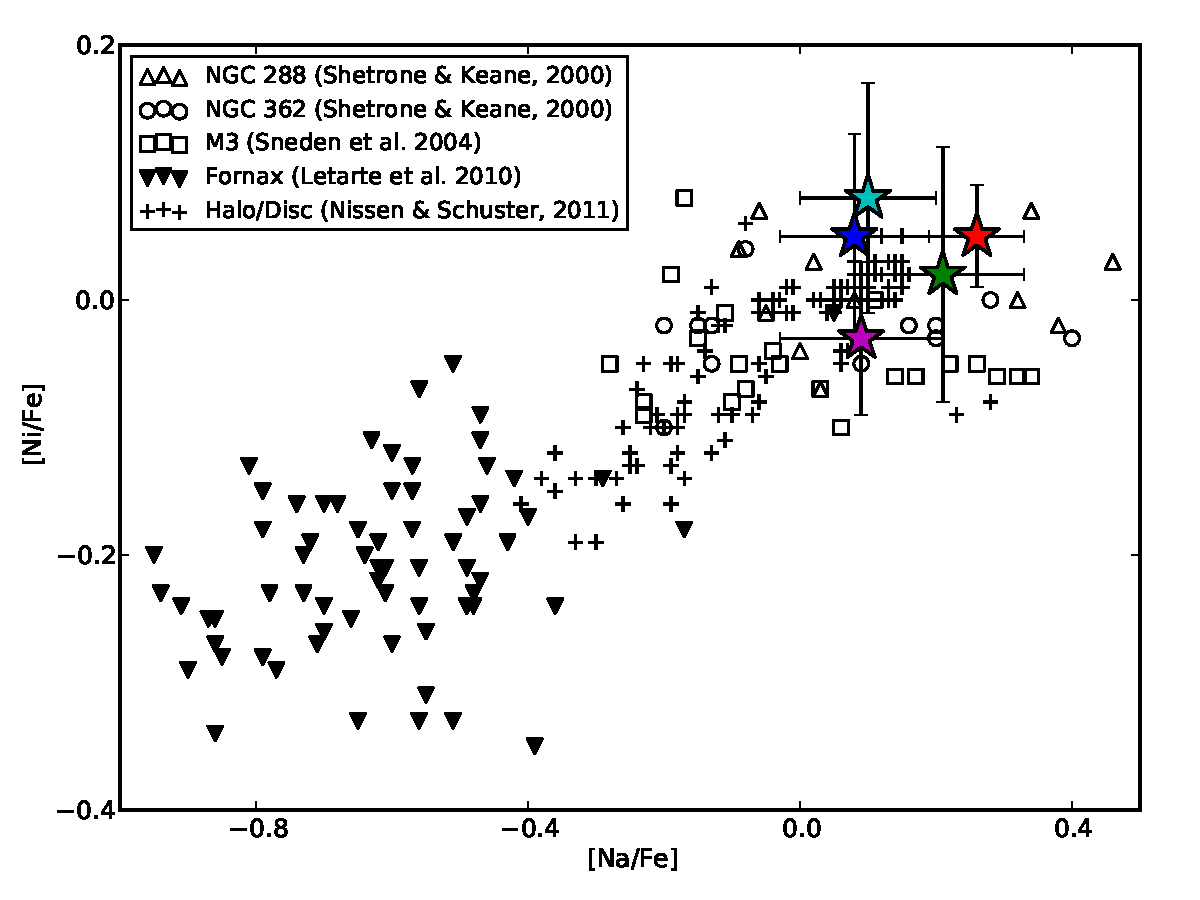
\includegraphics[width=\columnwidth]{./figures/gc-dsph-na-ni.pdf}
	\caption{[Na/Fe] and [Ni/Fe] for Aquarius stream stars and for globular cluster, dSph, and field (halo/disc) stars. Stars from the most representative dSph galaxy, Fornax, are shown as downward triangles ($\blacktriangledown$). The \citet{nissen;schuster_2011} plotted sample included halo stars, as well as low- and high-$\alpha$ disc members. As noted by \citet{nissen;schuster_1997,nissen;schuster_2011}, a positive Na-Ni relationship exists for field stars, with dSph members exhibiting strong depletion in both elements and globular cluster stars consistently showing an enhancement. Sodium and nickel content for Aquarius members indicate a dSph accretion origin is unlikely.}
	\label{fig:na-ni}
\end{figure}

Stars originating in dSph galaxies and globular clusters have very different chemical enrichment environments. Consequently, both types of systems exhibit chemistry that reflects their nucleosynthetic antiquity. Stars in dSphs do not demonstrate enhanced sodium or nickel content with respect to iron, as there has been a relatively small lineage of massive stars undergoing supernova. In contrast, globular cluster stars do have elevated [Na/Fe] and [Ni/Fe] signatures. This sharp contrast between dSph and globular cluster star chemistry is illustrated in Figure \ref{fig:na-ni}. Given the extended star formation within the Milky Way disc, globular cluster stars and disc stars are indiscernible in the Na/Ni plane: they both show an extended contribution of massive stars. The most that can be inferred from the Na and Ni abundances of Aquarius stream stars is that their enrichment environment is less like a dSph galaxy, and more representative of either a globular cluster, or the Milky Way disc. 


\subsection{The Chemically Peculiar Star C222531-145437}


%[TODO] Check this star in context of Verne & Smith for omega en
% --> Everything matches against D'Orazi (2011), Marino (2011), and Verne & Smith (2000) with the exception of Cu. But, it appears our Cu abundances are higher than the halo, too.

In almost every element with respect to iron, {C222531-145437} is distinct from the other Aquarius stream stars. It is over-abundant in light refractory  and neutron-capture elements, with a high barium abundance of {$\mbox{[Ba/Fe]} = 0.68$}. This value is well in excess of the halo ({$\mbox{[Ba/Fe]} \sim 0.0$}) -- and our other Aquarius stream stars -- which vary between $-$0.02 to {0.15\,dex}.

Here we discuss the possibility that an unseen companion has contributed to the surface abundances of C222531-145437. Although no radial velocity variations were observed between exposures, we do not have a sufficient baseline to detect such variation. The abundances of heavy elements produced by AGB stars have a high dependence on the initial metallicity and mass. Low-mass ($\lesssim{}3M_\odot$) AGB stars produce high fractions of heavy $s$-process elements compared to their light $s$-process counterparts. As such, [Ba/Y] is a useful indicator for considering contributions from a low-mass AGB companion. For C222531-145437, ${{\rm [Ba/Y]} = -0.17}$, which is much lower than expected if a low-mass AGB star was responsible for the heavy element enhancements ([Ba/Y] $\sim$ 0.5 as shown in Figure \ref{fig:ba-y}; see also \citet{cristallo;et-al_2009}). If mass transfer from an AGB companion has occurred very recently, non-negligible amounts of technetium are produced, remaining visible before it decays over $\sim$100\,Myr \citep{brown;et-al_1990,van_eck_jorrissen_1999, uttenthaler;et-al_2011}. We saw no technetium absorption at the 404.9, 423.8 or 429.7\,nm in the spectrum of C222531-145437. Intermediate-mass (3-5$M_\odot$) AGB stars also cannot explain the abundances for C222531-145437: using recently computed intermediate-mass AGB $s$-process yields for 3-5$M_\odot$ for a star of [Fe/H] = $-1.2$ (C. Fishlock, in preparation) the resulting surface abundances do not match the observations. Therefore, we find no reason to suspect the heavy element enhancement in C222531-145437 is the result of mass transfer from an AGB companion.

Stars in $\omega$-Centauri show large over-abundances of $s$-process elements compared to the Galaxy \citep{norris;da_costa_1995,stanford;et-al_2010}. M22 also hosts an $s$-process rich population \citep{marino;et-al_2011}. Like the Aquarius co-moving group, both clusters are relatively close to the Sun: {5.2\,kpc} and {3.2\,kpc}, respectively. M22 has a mean metallicity of {$\mbox{[Fe/H]} \sim -1.7$} and a range between {$-2.0 < \mbox{[Fe/H]} < -1.6$\,dex}, making an association between {C222531-145437} and M22 unlikely. Similarly, {C222531-145437} is unlikely to be associated with the metal-rich Argus association \citep[IC 2391;][]{de_silva;et-al_2013}, which also shows large enhancement in $s$-process abundances. Other groups have identified field stars enriched in $s$-process elements, which have generally been associated as tidal debris from $\omega$-Centuari \citep{wylie-de-boer;et-al_2010,majewski;et-al_2012}. The high $s$-process abundance ratios and overall metallicity of {C222531-145437} ({$\mbox{[Fe/H]} = -1.22$}) suggests this may be an additional tidal remnant. 

% [TODO] How do these abundances match omega Cen core RGB stars?

$\omega$-Centauri has a retrograde orbit with low inclination. Many groups simulating this orbit have predicted retrograde tidal debris to occur near the Solar circle \citep{dinescu_2002,tsuchiya_2003,tsuchiya_2004,bekki;freeman_2003}. Subsequent searches for $\omega$-Centauri debris in the Solar neighbourhood have led to tantalising signatures of debris. From over 4,000 stars targeted by \citet{da_costa;coleman_2008}, only six candidate debris members were recovered, consistent with tidal stripping occurring long ago. Using data from the Grid Giant Star Survey (GGSS), an all-sky search looking for metal-poor giant stars, \citet{majewski;et-al_2012} identified 12 stream candidates. In addition, \citet{majewski;et-al_2012} performed 4,050 simulations in order to predict likely locations for $\omega$-Centauri tidal debris. The results of their simulation are replicated in Figure \ref{fig:omega-cen-tidal-debris}, where the location of {C222531-145437} is also shown. The velocity and position of {C222531-145437} align almost precisely where \citet{majewski;et-al_2012} predict a high probability of tidal debris. More interestingly, the angular momentum and orbital energy for {C222531-145437} (Figure \ref{fig:Lz-E}) matches excellently for $\omega$-Centurai cluster stars as well as its previously identified tidal remnants \citep{wylie-de-boer;et-al_2010}. The chemical and phase-space information strongly suggests that {C222531-145437} is associated with the remnant of tidal stripping that occurred as the proto-$\omega$-Centauri fell into the Galaxy \citep{bekki;freeman_2003}.

\begin{figure}[h!]
	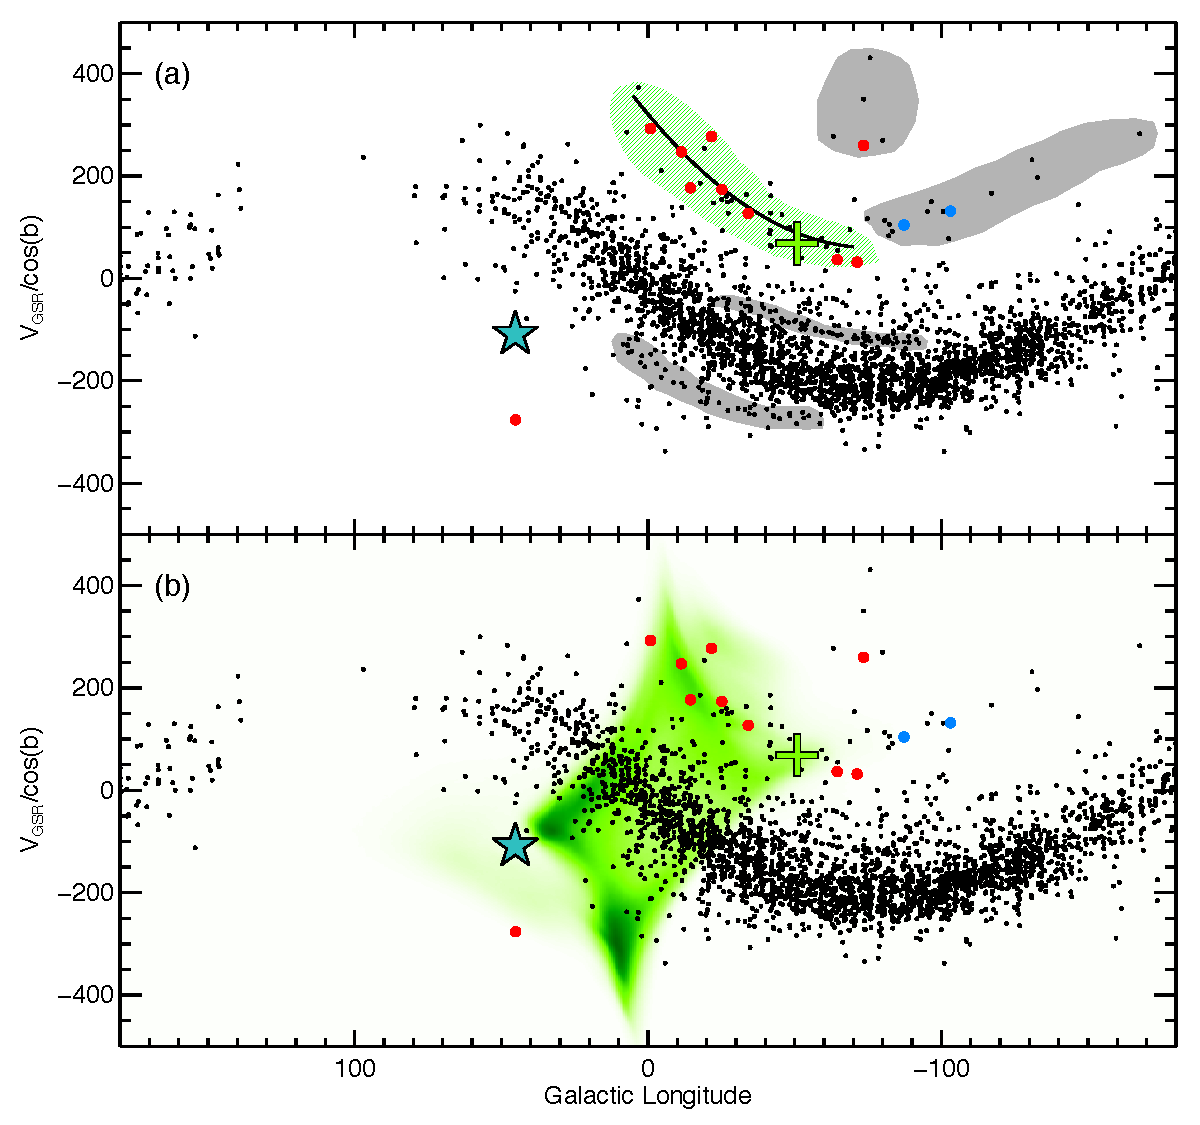
\includegraphics[width=\columnwidth]{./figures/omegacen_tidaldebris.pdf}
	\caption{Panel (a) shows the distribution of giant stars in the GGSS \citep{majewski;et-al_2012} in Galactic longitude and $V_{\rm GSR}/cos(b)$ after excluding stars with $|b| > 60^\circ$. Stars from the GGSS sample believed to be $\omega$-Centauri tidal debris are shown in green shading. Red points are stars from the GGSS sample with abundances that follow the $\omega$-Centauri [Ba/Fe]--[Fe/H] pattern. Blue points are those with high-resolution spectra that do not follow this trend. Grey shading highlights other potential halo substructures from their study. Panel (b) shows the probability distribution of $\omega$-Centauri tidal debris from 4,050 simulations.  The $\omega$-CenCentauri core is shown as a green cross and the cyan star represents {C222531-145437}, falling almost precisely where a relatively high probability of $\omega$-Centauri tidal debris is expected.}
	\label{fig:omega-cen-tidal-debris}
\end{figure}

% dynamics + orbital info


% Check this smith and dorazi paper 
%Furthermore, \textit{all other elemental abundances} measured here precisely match with those presented by \citet{smith;dorazi_2000} for $\omega$-Centauri RGB stars.

\begin{figure}[h!]
	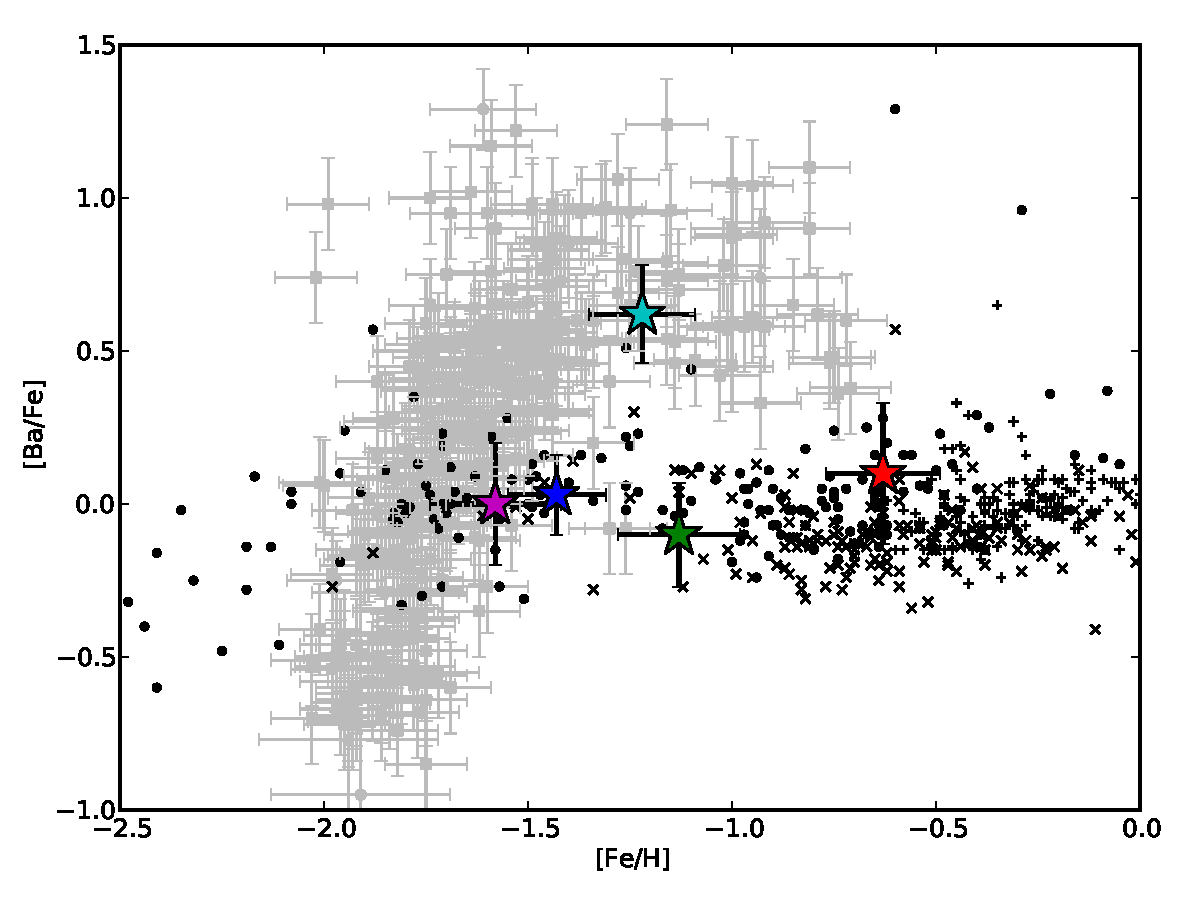
\includegraphics[width=\columnwidth]{./figures/omegaCen-c222531.pdf}
	\caption{[Fe/H] and [Ba/Fe] for halo/disc stars (black) from \citet{fulbright_2000,reddy;et-al_2003,reddy;et-al_2006} and $\omega$-Centauri RGB stars (grey) from \citet{francois;et-al_1988,smith;et-al_2000,marino;et-al_2011}. Similar trends are observed for other heavy elements in $\omega$-Centauri members. The candidate we associate with $\omega$-Centauri tidal debris, C222531-145437, is marked in cyan.}
	\label{fig:omega-cen-barium}
\end{figure}

% additional chemistry?
% [Sr/Ba] ~0.4

%The chemical peculiarity of {C222531-145437} suggests that it is distinct from the Aquarius co-moving group. The high $s$-process enrichment is similar to that observed in $\omega$-Centauri stars, and the overall metallicity {($\mbox{[Fe/H]} = -1.26$)} agrees excellently with the mean metallicity of a known sub-population within $\omega$-Centauri. Moreover, the position and velocity for {C222531-145437} precisely coincide with the most likely predictions for tidal debris from $\omega$-Centauri, and the angular momentum and orbital energy precisely matches those found for $\omega$-Centauri by \citet{dinescu;et-al_1999}. The chemical and phase-space information strongly suggests that {C222531-145437} is associated with the remnant of tidal stripping that occurred as the proto-$\omega$-Centauri fell into the Galaxy \citep{bekki;freeman_2003}.

In the Aquarius stream discovery paper, \citet{williams;et-al_2011} attempted to exclude possible known progenitors for the Aquarius stream. On the basis of metallicity, distance, proper motions, transverse velocities and orbital energies, the authors were able to exclude all known Milky Way satellites with the notable exception of $\omega$-Centauri. Although the Aquarius stream metallicity distribution is not dissimilar from a known sub-population in $\omega$-Centauri, the individual chemical abundances are quite distinct. The strong $s$-process enhancement with overall metallicity is not observed in the rest of our sample. Thus, with the exception of {C222531-145437}, the Aquarius members do not have a chemistry that is synonymous with $\omega$-Centauri tidal debris. It will be most interesting to learn how many other members of the Aquarius stream are tidal remnants of $\omega$-Centauri, given the frequency of these objects is quite low \citep[e.g. see][]{da_costa;coleman_2008,majewski;et-al_2012}.


\subsection{Disrupted Disc/Halo Stars -- Signature of a Disc-Satellite Interaction?}

%The stream members presented here are slightly enhanced in sodium and nickel, suggesting that if a satellite parent ever existed then its chemical enrichment environment was more like a globular cluster than a dSph galaxy. Stars currently present in existing dSph galaxies with metallicities similar to the Aquarius stream generally lack $\alpha$-enhancement, contrary to what is observed in the Aquarius stream. 

% When coupled with the observations of increased [Na/Fe] and [Ni/Fe] abundance ratios, this argues against the possibility that the Aquarius stream has resulted from a disrupted dSph like those that still exist today. If the progenitor is a disrupted globular cluster, and most of our candidates are members, then the parent has a wider metallicity distribution than almost every known globular cluster. 


Since the Aquarius stream is kinematically coherent, it has been assumed that the co-moving group has been accreted onto the Milky Way from a tidally disrupted satellite.  The chemical abundances presented in this study do not favour an accretion scenario from a globular cluster or a dSph; there is conflicting evidence for either hypothesis. As it stands, the co-moving group  appears chemically indistinguishable from thick disc/halo stars. These results force us to consider other scenarios that may replicate the observations.

The Aquarius stream has an unusually wide intrinsic velocity distribution. Generally a stellar stream is considered kinematically ``cold'' when its velocity dispersion is $\lesssim 8$\,km s$^{-1}$. We find the velocity dispersion from five members to be $\sim$30\,km\,s$^{-1}$, consistent with \citet{williams;et-al_2011}. Hypotheses invoked to explain the Aquarius co-moving group must account for the high velocity dispersion.
 
There are other co-moving groups in the Milky Way that were initially considered as tidal tails from disrupted satellites, that are now explainable as signatures of galaxy formation that are not specific accretion events. Like the Aquarius group, the Hercules moving group is significantly offset from the bulk of the observed velocity distribution. Members of the Hercules group exhibit a wide range of metallicities and ages \citep{bensby;et-al_2007, bovy;hogg_2010}. Furthermore, Hercules group stars have [X/Fe] abundance ratios at a given [Fe/H] that are {\it not} substantially different from the thin or thick disk. The Hercules group kinematics are well replicated in simulations by stars in the outer disc resonating with the bar in the central region of the Milky Way \citep{dehnen_2000,fux_2001}, and strong predictions are made for disc velocity distributions that would lend further weight to this hypothesis \citep{bovy_2010}. The Canis Major stellar over-density was also first considered to be an accretion feature from the postulated Canis Majoris dSph galaxy \citep{martin;et-al_2004}. However, \citet{momany;et-al_2004} demonstrate that the star counts, proper-motions, photometry and kinematics of the ``accreted feature'' can be easily explained by the warp and flare in the outer thick disc. The Monoceros ring \citep{newberg;et-al_2002,juric;et-al_2008} is perhaps another example of such an occurrence, as similar features naturally emerge as a consequence of galaxy-satellite interactions \citep{purcell;et-al_2011}, which has prompted considerable discussion \citep{lopez-corredoira;et-al_2012}. It is clear that not all kinematic groups are attributable to accretion events; in many scenarios a galactic origin is more likely, and simpler.

%We do not strongly consider the Aquarius co-moving group to be related to the flare and warp in the outer thick disc because near $l \sim 60\,^\circ$ the warp extends above the plane. Additionally the warp and flare of the disc is included in the Besan\c{c}on galaxy simulations \citep{robin;et-al_2003}, which were originally used to calculate the significance of the Aquarius over-density.

We hypothesise that the Aquarius group is the result of displaced stars from a perturbation in the thick disc. That is, the stars are Galactic in origin but have been displaced by a disc-satellite interaction. Minor mergers can significantly disrupt the host galaxy \citep{villalobos;helmi_2008}, producing extended spatial and kinematic structure in the process. \citet{minchev;et-al_2009} proposed that such a perturbation would cause a galactic ``ringing'' effect in the neighbourhood surrounding the merger site, analogous to the resulting compression wave propagating outwards from a stone falling in water. Stars move closer together in the wave peak, a signature which is observable in the velocities and orbital motions of nearby stars. This signature is most prominent in the $U$--$V$ velocity plane as concentric circles \citep{gomez;et-al_2012}, and dissolves over time (a few gigayear, depending on the mass of the perturber). After the $U$--$V$ velocity signature dissipates, a clear signature in angular momentum and orbital energy ($L_Z$, $E$) persists for long periods following the merger \citep[e.g. see][]{gomez;et-al_2012}.

Through Milky Way-Sagittarius simulations, \citet{purcell;et-al_2011} found that these disc-satellite interactions can explain ringing perturbations within the disc. Additionally, \citet{widrow;et-al_2012} and \citet{gomez;et-al_2012b} independently observed these phenomena -- a {\it``wavelike perturbation''}, as Widrow described -- in the SDSS and SEGUE catalogues. More recently, \citet{gomez;et-al_2013} proposed that these patterns were induced by the Sagittarius dSph interacting with the disc. Their simulations reproduce the observed north-south asymmetries and vertical wave-like structure, and show that the amplitude of these oscillations is strongly dependent on galactocentric distance. Combined with the oscillating vertical motions with the $U$--$V$ velocity pattern, corrugated waves are observed as a result of the interaction.

The stars in these oscillations should exhibit a wide range of ages, metallicities and a large spread in velocity dispersion. Thus, resultant oscillations following a disc-satellite interaction can satisfactorily explain the existence of the Aquarius co-moving group. We do not observe a distinct coherence in the $U$--$V$ velocity plane in our data, but the angular momentum and orbital energies for Aquarius members qualitatively reproduces the theoretically predicted pattern by \citet{gomez;et-al_2012} in a retrograde direction. The extent and gradient of this $L_Z$--$E$ signature is dependent on the mass of the perturber and the time since infall. Although our sample size is minute -- and the sample size would still be small even if all Aquarius members had reliable orbits -- the fact that we see no $U$--$V$ velocity coherence (Figure \ref{fig:toombre}) is consistent with the observed $L_Z$--$E$ pattern: signatures in the $L_Z$--$E$ plane (Figure \ref{fig:Lz-E}) become more extended over time as the $U$--$V$ signature dissipates. This is consistent with a disc-satellite interaction occurring in the disc approximately a few gigayear ago.

The Aquarius co-moving group resides at a an intermediate latitude ($b \approx -55^\circ$) and with a radial distance of up to $\sim$5\,kpc for some stars, the stars are slightly out of the plane. This is not inconsistent with a disc-satellite interaction. \citet{gomez;et-al_2013} find that a significant fraction of the total energy goes into vertical perturbations. While the mean vertical distance $\langle{}Z\rangle$ in their simulations are near zero, this is an average of disc particles at all plane heights -- positive and negative -- and the dispersions around $\langle{}Z\rangle$ are very large (F. G{\'o}mez, private communication, 2013). Moreover, \citet{gomez;et-al_2013} were only able to reliably track particles up to $|Z| \approx 1.4$\,kpc due to a finite number of particles in each cell volume.

% who is the perturber?
If the Aquarius group is a feature of a disc-satellite interaction, the perturber must have a mass on the order of a large globular cluster or a dSph satellite to produce the residual pattern in orbital energy and angular momenta. The Sagittarius dSph galaxy is an obvious candidate, but $\omega$-Centauri is also a possible perturber. On the basis on position, velocities, chemical abundances and orbit, we identify {C222531-145437} was highly likely stripped from $\omega$-Centauri in the past. Thus, it is plausible that $\omega$-Centauri has disrupted galactic stars as it passed through the plane, adding to any other oscillating modes rippling through the disc, resulting in what we now observe as the Aquarius stream.

\section{Conclusions}
\label{sec:conclusions}
We have presented a detailed chemical and dynamical analysis for 5 members of the recently discovered Aquarius stream from data taken with the MIKE spectrograph on the Magellan Clay telescope. Hereafter we solely refer to the discovery as a co-moving group instead of a stellar stream, as we find no evidence that the group is a tidal tail of a disrupted satellite. The main conclusions are as follows:

\begin{itemize}
\item The Aquarius stream is not mono-metallic. A wide spread in metallicities is observed, with [Fe/H] ranging from $-0.63$ to $-1.58$\,dex in just 5 members. 

\item No Na-O anti-correlation is observed in the Aquarius group. Two members have slightly enhanced levels of sodium with respect to iron. If the candidates were \textit{known globular cluster members}, they would be classified as belonging to either the primordial component, or at most, tenuous membership could be argued for the lower envelope of the intermediate group.

\item We find a strong positive Mg-Al relationship, reminiscent of Milky Way field stars and contrary to globular cluster observations. 

\item We find no evidence that the Aquarius group is the result of a disrupted classical globular cluster. The large [Fe/H] variation severely limits the number of possible parent hosts, and both the extreme and intermediate component of the Na-O anti-correlation have not been observed. In total, high-resolution spectra exists for more than half of the stream.

\item The co-moving group shows an $\alpha$-enhancement of ${[\alpha/{\rm Fe}] = +0.40}$\,dex, similar to the Milky Way, and distinct to that typically observed in stars in dSph galaxies with comparable metallicities.

\item Aquarius members are enhanced in [Na/Fe] and [Ni/Fe] to levels typically observed in either the thick disc or globular clusters. These levels of [Na/Fe] and [Ni/Fe] enhancement are not observed in stars from dSph galaxies. Low [Ba/Y] abundance ratios are also observed in the Aquarius group, in conflict with chemistry of present day dSph galaxies. Thus, on the basis of [(Na, Ni, $\alpha$)/Fe] and [Ba/Y] abundance ratios, it is unlikely the Aquarius co-moving group is the result of a tidally disrupted dSph galaxy.

% [TODO] what about C222531 in other elements with omega-Cen?

\item One of our candidates, {C222531-145437}, has an abundance pattern that is clearly distinct from the other Aquarius members, most notably in barium where {[Ba/Fe] = 0.68}\,dex. We exclude the possibility that the abundance variations have resulted from an AGB companion.

\item The position and velocity {C222531-145437} coincides precisely where simulations by \citet{majewski;et-al_2012} predict large amounts of $\omega$-Centauri tidal debris, and the orbital energy and angular momenta are consistent with the $\omega$-Centauri cluster. The chemical and phase-space information suggests that {C222531-145437} is a rare tidal debris member of the globular cluster $\omega$-Centauri. Removing C222531-145437 from the Aquarius sample does not extinguish or diminish any of the aforementioned conclusions.

\item While no evidence exists for an accreted origin, and the Aquarius group members are indistinguishable from thick disc/halo stars, we hypothesise the co-moving group is the result from a disc-satellite interaction. We see no coherent pattern in the $U$--$V$ plane from Monte-Carlo simulations, but the orbital energies and angular momenta for the Aquarius group qualitatively reproduces patterns predicted by \citet{gomez;et-al_2012}. This is consistent with a minor merger in the Milky Way thick disc occurring perhaps up to a few gigayear ago. Given the location and velocity of the Aquarius group, and the identification of {C222531-145437} as a star tidally stripped from $\omega$-Centauri, it is plausible that the Milky Way-$\omega$Cen interaction sufficiently perturbed outer disc/halo stars to produce what we now observe as the Aquarius group.
\end{itemize}

It is clear that not all co-moving groups are tidal tails of disrupted satellites, and that the structure of the Milky Way is indeed complex. While we find no chemical evidence that the Aquarius group is a tidal tail from a disrupted satellite, we propose the members are Galactic in origin, and the co-moving group is a result of a disc-satellite interaction. Thus, although the Aquarius group has not been accreted onto the galaxy, it certainly adds to the rich level of kinematic substructure within the Milky Way.

\acknowledgements
We are indebted to David Nidever and Steven Majewski for kindly replicating a plot from their $\omega$-Centauri simulations (Figure \ref{fig:omega-cen-tidal-debris} in this text) which helped to place {C222531-145437} in context of the cluster's tidal debris. A.R.C. acknowledges the financial support through the Australian Research Council Laureate Fellowship LF0992131, and from the Australian Prime Minister's Endeavour Award Research Fellowship, which facilitated his research at MIT. This publication makes use of data products from the Two Micron All Sky Survey, which is a joint project of the University of Massachusetts and the Infrared Processing and Analysis Center/California Institute of Technology, funded by the National Aeronautics and Space Administration and the National Science Foundation. \\

% [TODO] Stellar parameter uncertainties
% [TODO] Chemical abundance uncertainties


%\facilities{Magellan:Clay}

\bibliographystyle{apj}
\bibliography{bibliography}

\end{document}